\documentclass[12pt,a4paper]{report}

% ── Packages ──────────────────────────────────────────────────────────────────
\usepackage[utf8]{inputenc}
\usepackage[T1]{fontenc}
\usepackage[english]{babel}
\usepackage{geometry}
\usepackage{graphicx}
\usepackage{booktabs}
\usepackage{longtable}
\usepackage{array}
\usepackage{xcolor}
\usepackage{hyperref}
\usepackage{enumitem}
\usepackage{titlesec}
\usepackage{fancyhdr}
\usepackage{parskip}
\usepackage{microtype}
\usepackage{caption}
\usepackage{float}
\usepackage{tabularx}
\usepackage{multirow}
\usepackage{lmodern}
\usepackage{ragged2e}
\PassOptionsToPackage{hyphens}{url}

% ── Allow extra inter-word stretch to avoid hbox overflows ────────────────────
\setlength{\emergencystretch}{3em}
\hbadness=10000

% ── Page geometry ─────────────────────────────────────────────────────────────
\geometry{top=2.5cm, bottom=2.5cm, left=2.8cm, right=2.8cm}

% ── Image search path ─────────────────────────────────────────────────────────
\graphicspath{{report_images/}{images/}}

% ── Colours ───────────────────────────────────────────────────────────────────
\definecolor{uagreen}{RGB}{0,150,57}
\definecolor{detiblue}{RGB}{0,112,192}
\definecolor{sevcritical}{RGB}{192,0,0}
\definecolor{sevhigh}{RGB}{255,102,0}
\definecolor{sevmedium}{RGB}{180,140,0}
\definecolor{sevlow}{RGB}{0,140,60}
\definecolor{codegray}{RGB}{245,245,245}

% ── Hyperref ──────────────────────────────────────────────────────────────────
\hypersetup{
  colorlinks=true,
  linkcolor=detiblue,
  urlcolor=detiblue,
  citecolor=detiblue,
  pdftitle={Security in Software Engineering -- Group 102},
  pdfauthor={Tomás Brás, Afonso Ferreira},
}

% ── Section title formatting ──────────────────────────────────────────────────
\titleformat{\chapter}[display]
  {\normalfont\Large\bfseries\color{detiblue}}
  {\chaptertitlename\ \thechapter}{10pt}{\Huge}
\titleformat{\section}
  {\normalfont\large\bfseries\color{detiblue}}{\thesection}{1em}{}
\titleformat{\subsection}
  {\normalfont\normalsize\bfseries\color{detiblue!80}}{\thesubsection}{1em}{}
\titleformat{\subsubsection}
  {\normalfont\normalsize\itshape\color{detiblue!70}}{\thesubsubsection}{1em}{}

% ── Header / footer ───────────────────────────────────────────────────────────
\pagestyle{fancy}
\fancyhf{}
\fancyhead[L]{\small\textit{Security in Software Engineering -- Group 102}}
\fancyhead[R]{\small\textit{Universidade de Aveiro}}
\fancyfoot[C]{\thepage}
\renewcommand{\headrulewidth}{0.4pt}

% ── Severity badge helpers ────────────────────────────────────────────────────
\newcommand{\critical}{\textbf{\textcolor{sevcritical}{Critical}}}
\newcommand{\high}{\textbf{\textcolor{sevhigh}{High}}}
\newcommand{\medium}{\textbf{\textcolor{sevmedium}{Medium}}}
\newcommand{\low}{\textbf{\textcolor{sevlow}{Low}}}

% ── Helper: STRIDE row columns
% 5 cols: ID | Threat | Component | Severity | Detail
% widths: 0.9 | 3.6 | 2.8 | 1.9 | 4.8  => 14.0cm + separators ≈ ok
\newcolumntype{S}[1]{>{\RaggedRight\arraybackslash}p{#1}}

% ──────────────────────────────────────────────────────────────────────────────
\begin{document}

% ── Title page ────────────────────────────────────────────────────────────────
\begin{titlepage}
  \centering
  % logos
  \begin{minipage}[c]{0.45\textwidth}
    
\includegraphics[height=2cm]{uni.png}
  \end{minipage}
  \hfill
  \begin{minipage}[c]{0.45\textwidth}
    \raggedleft
    
\includegraphics[height=2cm]{deti.png}
  \end{minipage}

  \vspace{0.6cm}
  {\color{uagreen}\rule{\linewidth}{3pt}}\\[0.4cm]
  {\Large\bfseries Universidade de Aveiro}\\[0.1cm]
  {\large Departamento de Electrónica, Telecomunicações e Informática}\\[0.4cm]
  {\color{uagreen}\rule{\linewidth}{3pt}}

  \vspace{3cm}
  {\Huge\bfseries Security in Software Engineering}\\[0.6cm]
  {\Large Threat Modelling, SAST \& DAST Report}\\[0.4cm]
  {\large\itshape Group 102}

  \vspace{3cm}
  \begin{tabular}{rl}
    \textbf{Tomás Brás}      & N\textsuperscript{o} 112665 \\[4pt]
    \textbf{Afonso Ferreira} & N\textsuperscript{o} 113480 \\
  \end{tabular}

  \vfill
  {\large\today}\\[0.4cm]
  {\color{uagreen}\rule{\linewidth}{2pt}}
\end{titlepage}

% ── Table of contents ─────────────────────────────────────────────────────────
\tableofcontents
\clearpage

% ══════════════════════════════════════════════════════════════════════════════
\chapter{Threat Modelling -- Context and Objectives}
% ══════════════════════════════════════════════════════════════════════════════

This threat model covers the full-stack clinic management application composed of a React/Vite frontend, a Spring Boot backend, and a PostgreSQL database, orchestrated via Docker Compose. The system manages patient and appointment data for a medical clinic.

\textbf{Security objectives:}
\begin{itemize}
  \item Protect patient health and contact data (PII/PHI) from unauthorised disclosure.
  \item Prevent unauthorised creation, modification, or deletion of patient and appointment records.
  \item Maintain availability of the system for clinic staff.
  \item Ensure data integrity of medical records.
\end{itemize}

\textbf{Out of scope:} Network-level infrastructure, physical security, and end-user workstations.

% ─────────────────────────────────────────────────────────────────────────────
\section{System Description}
% ─────────────────────────────────────────────────────────────────────────────

\begin{table}[H]
\centering
\caption{System components and exposure levels}
\begin{tabularx}{\linewidth}{l X l}
\toprule
\textbf{Component} & \textbf{Technology} & \textbf{Exposure} \\
\midrule
Frontend      & React 19 + Vite 7, Node dev server           & Public (browser) \\
Backend       & Java 21 + Spring Boot 4.0.2, port 8080       & Host-exposed, proxied via Vite \\
Database      & PostgreSQL 16                                 & Internal only \\
Orchestration & Docker Compose                                & Host only \\
\bottomrule
\end{tabularx}
\end{table}

\textbf{Key observations with security relevance:}
\begin{itemize}
  \item No authentication or authorisation layer exists anywhere in the baseline stack.
  \item Backend binds JPA entities directly from HTTP request bodies (no DTOs, no \texttt{@Valid}).
  \item Frontend runs as a dev server (\texttt{npm run dev}) inside Docker -- not a production build.
  \item Auto-seeder populates 120 patients and 520 appointments on empty database startup.
  \item \texttt{patientId} is passed as a query parameter when creating appointments.
  \item \texttt{PUT /api/appointments/\{id\}} allows re-assigning a patient via body \texttt{\{"patient":\{"id":X\}\}}.
  \item \texttt{PatientRepository.findByEmail()} exists but is unused -- email uniqueness is not enforced.
  \item SPECIALTIES and STATUSES are duplicated between frontend and backend with no server-side enum validation.
  \item No server-side pagination, rate limiting, or audit logging is implemented.
\end{itemize}

% ─────────────────────────────────────────────────────────────────────────────
\section{Assets}
% ─────────────────────────────────────────────────────────────────────────────

\begin{itemize}
  \item \textbf{Patient PII} -- name, date of birth, phone number, and email.
  \item \textbf{Appointment records} -- date and time, specialty, status, and patient linkage.
  \item \textbf{Database credentials} -- used by the backend to access PostgreSQL.
  \item \textbf{System availability} -- necessary for normal clinic operation.
  \item \textbf{Audit trail} -- currently absent, representing an additional risk.
\end{itemize}

% ─────────────────────────────────────────────────────────────────────────────
\section{Trust Boundaries}
% ─────────────────────────────────────────────────────────────────────────────

\begin{description}
  \item[\textbf{TB-1: HTTP/Browser Boundary}] No TLS or authentication is used in the current setup.
  \item[\textbf{TB-2: Vite Proxy Boundary}] \texttt{/api} requests are forwarded without authentication or access checks.
  \item[\textbf{TB-3: JPA/JDBC Boundary}] The backend connects to PostgreSQL with a single read/write account and no row-level security.
\end{description}

\begin{figure}[H]
  \centering
  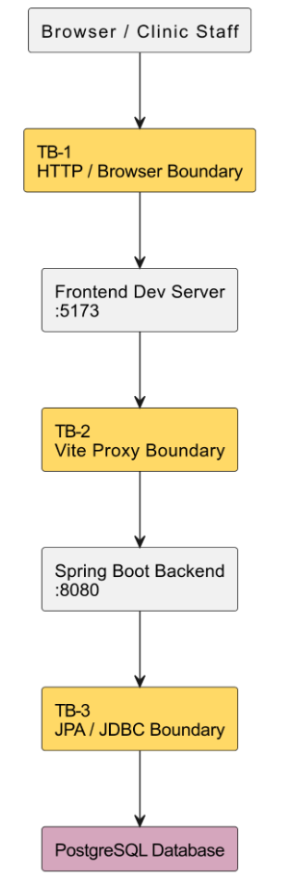
\includegraphics[width=0.40\linewidth]{assets.png}
  \caption{System trust boundary stack (TB-1 to TB-3)}
\end{figure}

% ─────────────────────────────────────────────────────────────────────────────
\section{Data Flow Diagrams}
% ─────────────────────────────────────────────────────────────────────────────

\subsection{DFD Notation}

The diagrams use standard DFD-inspired notation:
\begin{description}
  \item[\textbf{Rectangle}] External entity (the Patient).
  \item[\textbf{Circle}] Process -- Manage Patient Data, Manage Appointments, Search and View Information.
  \item[\textbf{Cylinder}] Data store -- D1 Patient Records, D2 Appointment Records.
  \item[\textbf{Arrow}] Data flow between entities, processes, and stores.
\end{description}

\subsection{Level 0 -- Context Diagram}

The Level 0 DFD presents the entire application as a single process. The external entity is the Patient, two trust boundaries are identified (TB-1 between Patient and the system, TB-3 between the system and the database).

\begin{figure}[H]
  \centering
  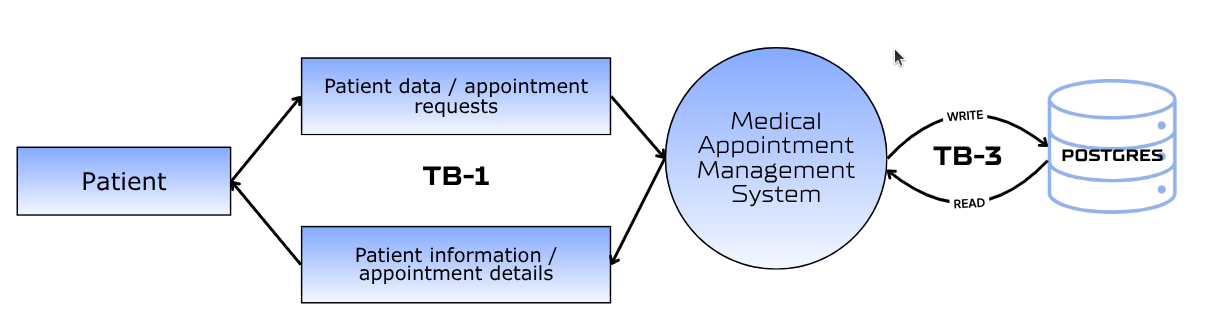
\includegraphics[width=0.75\linewidth]{DFD0.png}
  \caption{DFD Level 0 -- Context Diagram}
\end{figure}

\subsection{Level 1 -- System Decomposition}

The Level 1 DFD decomposes the system into three internal sub-processes:
\begin{itemize}
  \item 1.0 Manage Patient Data
  \item 2.0 Manage Appointments
  \item 3.0 Search and View Information
\end{itemize}

\begin{figure}[H]
  \centering
  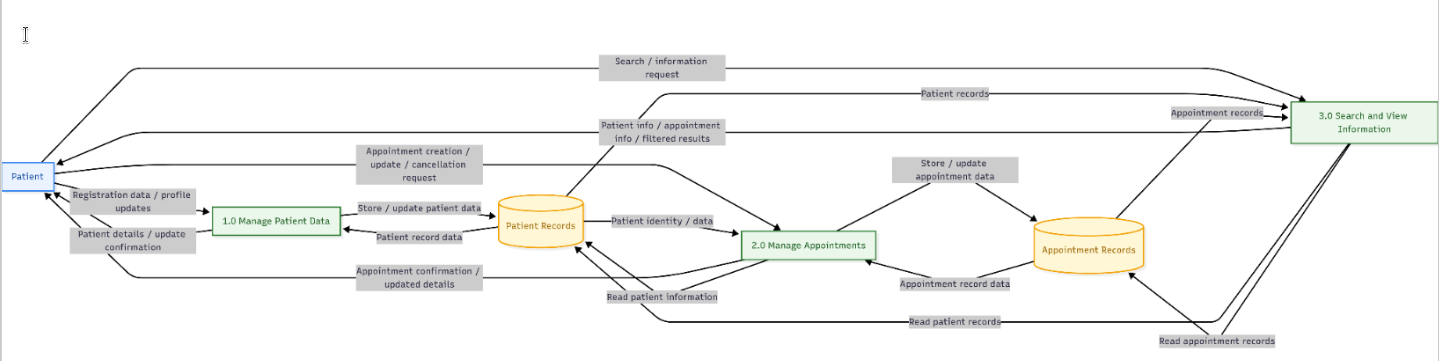
\includegraphics[width=\linewidth]{DFD1.png}
  \caption{DFD Level 1 -- System Decomposition}
\end{figure}

\subsection{Level 2 -- Detailed View of Appointment Creation}

The Level 2 view focuses on the Appointment Creation Flow, covering Patient, AppointmentController, AppointmentService, PatientRepository, AppointmentRepository, and Database.

Main steps:
\begin{enumerate}
  \item The patient sends \texttt{POST /api/appointments?patientId=ID}.
  \item The controller forwards the request to the service layer.
  \item The service validates the patient by checking \texttt{patientId}.
  \item If the patient exists, the appointment is saved and HTTP 201 is returned.
  \item If the patient does not exist, HTTP 404 is returned.
\end{enumerate}

\begin{figure}[H]
  \centering
  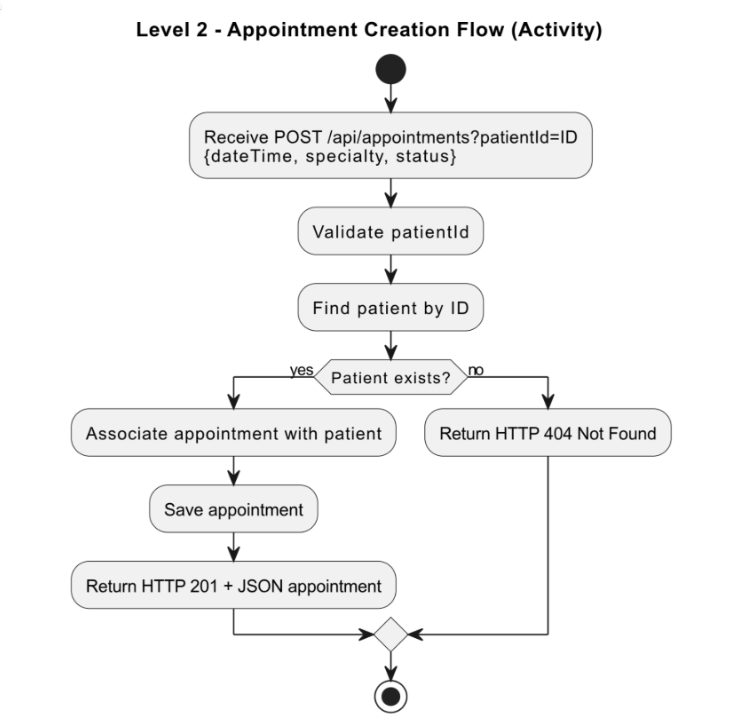
\includegraphics[width=0.75\linewidth]{DFD2.png}
  \caption{DFD Level 2 -- Appointment Creation (activity diagram)}
\end{figure}

\begin{figure}[H]
  \centering
  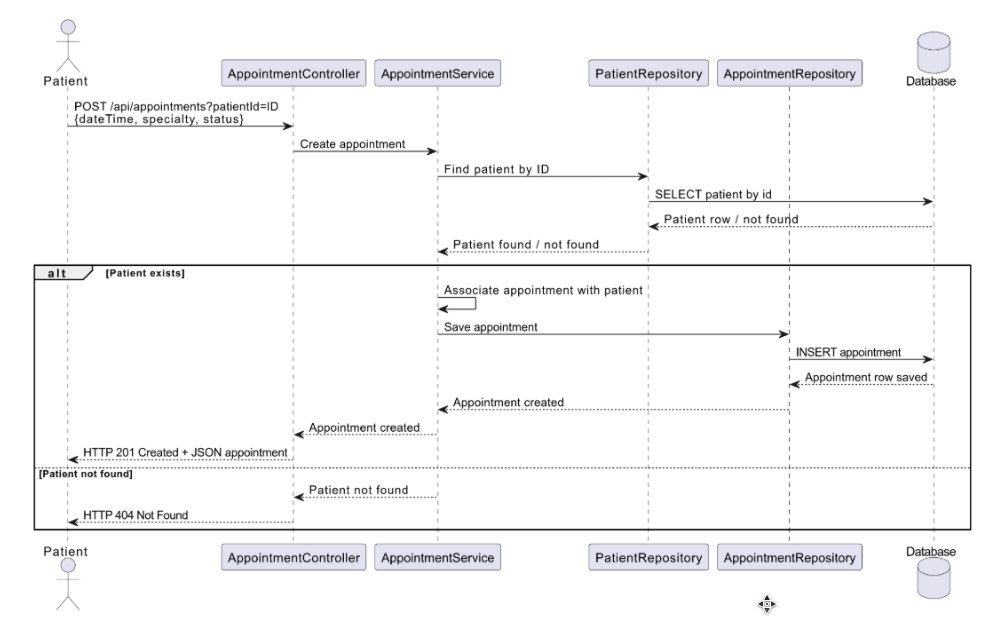
\includegraphics[width=\linewidth]{FLOW2.png}
  \caption{DFD Level 2 -- Appointment Creation (sequence diagram)}
\end{figure}

% ─────────────────────────────────────────────────────────────────────────────
\section{Approach}
% ─────────────────────────────────────────────────────────────────────────────

This project uses both \textbf{LINDDUN} and \textbf{STRIDE} as complementary threat modelling methodologies. LINDDUN covers privacy risks (identifiability, linkability, disclosure, inference of health patterns), while STRIDE covers broader security threats (spoofing, tampering, repudiation, information disclosure, denial of service, elevation of privilege).

% ─────────────────────────────────────────────────────────────────────────────
\section{LINDDUN Analysis}
% ─────────────────────────────────────────────────────────────────────────────

\begin{longtable}{>{\bfseries}S{2.8cm} S{1.6cm} S{4.8cm} S{4.4cm}}
\caption{LINDDUN privacy threat analysis}\label{tab:linddun}\\
\toprule
\textbf{Category} & \textbf{Relevance} & \textbf{Description} & \textbf{Detail} \\
\midrule
\endfirsthead
\multicolumn{4}{l}{\small\textit{(continued)}}\\
\toprule
\textbf{Category} & \textbf{Relevance} & \textbf{Description} & \textbf{Detail} \\
\midrule
\endhead
\bottomrule
\endfoot

Identifiability & \high & Patients can be directly identified from stored records (name, email, phone, date of birth). & All fields returned via \texttt{GET /api/patients}. Sequential IDs make enumeration trivial. \\[6pt]

Linkability & \high & Patient identity can be linked to appointment records, enabling inference of health patterns. & Appointment is linked to Patient. Search filters by \texttt{patientName}, \texttt{date}, \texttt{status}, \texttt{specialty} -- all without authentication. \\[6pt]

Disclosure of Information & \high & Unauthenticated endpoints expose full patient and appointment data. & \texttt{GET /api/patients} and \texttt{GET /api/appointments} require no credentials. \\[6pt]

Detectability & \medium & An attacker can confirm whether a named individual is a patient via API responses. & Sequential IDs and 200/404 differences on \texttt{/\{id\}} endpoints expose record existence. \\[6pt]

Non-repudiation & \medium & No authentication or audit logging -- data access and modifications cannot be attributed. & No session tracking or audit events. Any CRUD operation is permanently unattributable. \\[6pt]

Unawareness & \medium & Patients have no way to know how their data is processed or to exercise their rights. & No consent flow, privacy notice, or rights-handling workflow. GDPR Articles 15--17 cannot be fulfilled. \\[6pt]

Non-compliance & \high & Structural GDPR violations applicable to health data expose the clinic to regulatory liability. & No lawful basis for processing; no explicit consent; no retention policy; no breach notification. \\
\end{longtable}

% ─────────────────────────────────────────────────────────────────────────────
\section{STRIDE Threat Analysis}
% ─────────────────────────────────────────────────────────────────────────────

\subsection{Spoofing}

\begin{table}[H]
\centering
\caption{Spoofing threats}
\begin{tabularx}{\linewidth}{S{0.8cm} S{3.2cm} S{2.4cm} S{2.1cm} X}
\toprule
\textbf{ID} & \textbf{Threat} & \textbf{Component} & \textbf{Severity} & \textbf{Detail} \\
\midrule
S-01 & Any user can impersonate any clinic staff member -- \textbf{no authentication exists}. & Backend API & \critical & No Spring Security configuration or auth middleware is present anywhere in the stack. \\[6pt]
S-02 & Attacker can forge \texttt{patientId} query parameter to create appointments under any patient. & Appointment API & \high & The controller accepts \texttt{patientId} from the request and the service trusts it after \texttt{findById()}. \\
\bottomrule
\end{tabularx}
\end{table}

\subsection{Tampering}

\begin{table}[H]
\centering
\caption{Tampering threats}
\begin{tabularx}{\linewidth}{S{0.8cm} S{3.2cm} S{2.4cm} S{2.1cm} X}
\toprule
\textbf{ID} & \textbf{Threat} & \textbf{Component} & \textbf{Severity} & \textbf{Detail} \\
\midrule
T-01 & Any unauthenticated user can PUT to \texttt{/api/\allowbreak{}appointments/\allowbreak{}\{id\}} and change patient linkage, date, status, or specialty. & Appointment API & \critical & The appointment update service updates all mutable fields and can silently swap the linked patient. \\[6pt]
T-02 & Any unauthenticated user can PUT to \texttt{/api/\allowbreak{}patients/\allowbreak{}\{id\}} and modify patient PII. & Patient API & \critical & The patient update service directly replaces name, date of birth, phone number, and email. \\[6pt]
T-03 & Direct entity binding accepts nested relationship data from clients. & Backend (no DTOs) & \medium & Controllers deserialise directly into JPA entities instead of constrained request DTOs. \\[6pt]
T-04 & SPECIALTIES and STATUSES not validated server-side -- arbitrary strings can be persisted. & Appointment entity & \medium & \texttt{specialty} and \texttt{status} are plain String fields with no enum or bean validation. \\[6pt]
T-05 & Email field has no uniqueness constraint enforced by the application. & Patient API & \medium & \texttt{findByEmail()} exists in the repository but is unused during create or update flows. \\
\bottomrule
\end{tabularx}
\end{table}

\subsection{Repudiation}

\begin{table}[H]
\centering
\caption{Repudiation threats}
\begin{tabularx}{\linewidth}{S{0.8cm} S{3.2cm} S{2.4cm} S{2.1cm} X}
\toprule
\textbf{ID} & \textbf{Threat} & \textbf{Component} & \textbf{Severity} & \textbf{Detail} \\
\midrule
R-01 & No audit logging -- any CRUD operation leaves no trace. & Entire backend & \high & No audit service, interceptor, event sink, or change history is implemented. \\[6pt]
R-02 & No authentication means no actor identity is ever recorded in logs. & Entire system & \critical & Requests are anonymous end-to-end; server logs cannot attribute actions to any real actor. \\[6pt]
R-03 & Cascade delete on Patient removes all linked appointments with no log or recovery path. & Patient delete API & \high & Patient uses \texttt{CascadeType.ALL} and \texttt{orphanRemoval = true} on appointments. \\
\bottomrule
\end{tabularx}
\end{table}

\subsection{Information Disclosure}

\begin{table}[H]
\centering
\caption{Information Disclosure threats}
\begin{tabularx}{\linewidth}{S{0.8cm} S{3.2cm} S{2.4cm} S{2.1cm} X}
\toprule
\textbf{ID} & \textbf{Threat} & \textbf{Component} & \textbf{Severity} & \textbf{Detail} \\
\midrule
I-01 & Full patient PII returned in all \texttt{GET /api/patients} responses -- no field-level filtering or RBAC. & Patient API & \high & The API returns entity objects directly, including PII and linked appointment collections. \\[6pt]
I-02 & No pagination -- \texttt{GET /api/patients} returns all 120+ records in one response. & Patient API & \medium & \texttt{PatientService.getAll()} calls \texttt{findAll()} with no limit, page, or field projection. \\[6pt]
I-03 & Unhandled error responses may disclose implementation details. & Backend & \low & No explicit production error-handling policy is configured in the repository. \\[6pt]
I-04 & Database credentials stored in \texttt{.env} file -- leaked if repo is made public. & Config & \high & \texttt{docker-compose.yml} reads \texttt{POSTGRES\_USER} and \texttt{POSTGRES\_PASSWORD} from the \texttt{.env} file. \\[6pt]
I-05 & Dev server (\texttt{npm run dev}) exposes development assets and implementation details. & Frontend container & \medium & The frontend runs Vite directly instead of a production build through a hardened web server. \\[6pt]
I-06 & Backend port 8080 may be directly accessible, bypassing the Vite proxy. & Docker networking & \medium & \texttt{docker-compose.yml} publishes the backend port to the host, not only the internal Docker network. \\
\bottomrule
\end{tabularx}
\end{table}

\subsection{Denial of Service}

\begin{table}[H]
\centering
\caption{Denial of Service threats}
\begin{tabularx}{\linewidth}{S{0.8cm} S{3.2cm} S{2.4cm} S{2.1cm} X}
\toprule
\textbf{ID} & \textbf{Threat} & \textbf{Component} & \textbf{Severity} & \textbf{Detail} \\
\midrule
D-01 & No rate limiting -- attacker can flood \texttt{POST /api/appointments} to exhaust DB connections. & Backend API & \high & No throttling, quota, or back-pressure mechanism at any layer. \\[6pt]
D-02 & No pagination on \texttt{GET /api/appointments} -- large result sets can exhaust memory. & Appointment search & \medium & The appointment repository returns the full matching set in memory with no page limit. \\[6pt]
D-03 & \texttt{DELETE /api/patients/\{id\}} cascades to all appointments -- one request can delete hundreds of records. & Patient delete & \high & A single patient deletion removes the parent record and all dependent appointments. \\
\bottomrule
\end{tabularx}
\end{table}

\subsection{Elevation of Privilege}

\begin{table}[H]
\centering
\caption{Elevation of Privilege threats}
\begin{tabularx}{\linewidth}{S{0.8cm} S{3.2cm} S{2.4cm} S{2.1cm} X}
\toprule
\textbf{ID} & \textbf{Threat} & \textbf{Component} & \textbf{Severity} & \textbf{Detail} \\
\midrule
E-01 & No roles or permissions -- all API operations are equally accessible to any caller. & Entire backend & \critical & No RBAC, ownership check, or record-level authorisation anywhere in the backend. \\[6pt]
E-02 & Client-controlled nested objects can influence backend relationships during updates. & Backend (no DTOs) & \high & The update flow trusts nested \texttt{patient.id} in request bodies to change appointment ownership. \\[6pt]
E-03 & \texttt{PUT /api/\allowbreak{}appointments/\allowbreak{}\{id\}} re-assigns patient -- allows transferring medical records between patients. & Appointment service & \high & The update service resolves the provided patient ID and rebinds the appointment to a different patient if found. \\
\bottomrule
\end{tabularx}
\end{table}

% ─────────────────────────────────────────────────────────────────────────────
\section{Abuse Cases}
% ─────────────────────────────────────────────────────────────────────────────

Privacy and security threats were identified using the LINDDUN framework, suited for systems processing personal and health-related data.

\textbf{LINDDUN categories used:} Linking $\cdot$ Identifying $\cdot$ Non-repudiation $\cdot$ Detecting $\cdot$ Disclosure $\cdot$ Unawareness $\cdot$ Non-compliance.

\subsection*{AS-01 -- Unauthorised Access to Patient Data}
\begin{table}[H]
\begin{tabularx}{\linewidth}{>{\bfseries\RaggedRight\arraybackslash}p{2.6cm} X}
\toprule
LINDDUN   & Disclosure -- \critical \\\midrule
Abuse Case & As a malicious external user, I want to access another patient's personal data so that I can obtain sensitive information such as name, email, phone number, date of birth, and linked appointment data. \\\midrule
How        & The attacker sends direct requests to \texttt{/api/patients} and \texttt{/api/\allowbreak{}appointments} and retrieves records without any access control, as no authentication mechanism exists in the system. \\\midrule
Impact     & Exposure of personal and appointment-related data, leading to a privacy breach. \\
\bottomrule
\end{tabularx}
\end{table}

\subsection*{AS-02 -- Link Patient Identity to Appointment History}
\begin{table}[H]
\begin{tabularx}{\linewidth}{>{\bfseries\RaggedRight\arraybackslash}p{2.6cm} X}
\toprule
LINDDUN   & Linking -- \critical \\\midrule
Abuse Case & As a malicious external user, I want to associate patient identity data with appointment records so that I can infer sensitive patterns such as recurring specialties and possible health-related conditions. \\\midrule
How        & The attacker correlates the full patient list with appointment records through linked identifiers. Both endpoints are unauthenticated and return all records without pagination, making full profiling possible in two requests. \\\midrule
Impact     & Sensitive health patterns can be inferred from metadata alone, increasing patient profiling risk beyond what any single record reveals. \\
\bottomrule
\end{tabularx}
\end{table}

\subsection*{AS-03 -- Directly Identify a Patient from Stored Records}
\begin{table}[H]
\begin{tabularx}{\linewidth}{>{\bfseries\RaggedRight\arraybackslash}p{2.6cm} X}
\toprule
LINDDUN   & Identifying -- \critical \\\midrule
Abuse Case & As a malicious external user, I want to use personal identifiers stored in the system so that I can directly identify a patient and associate their appointment information with a real individual. \\\midrule
How        & The attacker accesses records containing direct identifiers (name, email, phone, date of birth). Patient IDs are sequential integers starting at 1, making full enumeration via \texttt{/api/patients/\{id\}} trivial with no rate limiting or authentication. \\\midrule
Impact     & A real individual can be directly identified and their full appointment history retrieved. \\
\bottomrule
\end{tabularx}
\end{table}

\subsection*{AS-04 -- Infer a Patient's Health Condition from Appointment Metadata}
\begin{table}[H]
\begin{tabularx}{\linewidth}{>{\bfseries\RaggedRight\arraybackslash}p{2.6cm} X}
\toprule
LINDDUN   & Detecting -- \critical \\\midrule
Abuse Case & As a malicious external user, I want to observe the specialty and status fields of a patient's appointments so that I can infer sensitive health information without ever accessing a medical record directly. \\\midrule
How        & The attacker filters \texttt{GET /api/\allowbreak{}appointments?patientName=X} to retrieve the full appointment history. Repeated ``Psychiatry'' visits with status \texttt{NO\_SHOW} reveal sensitive patterns without any explicit diagnosis data. \\\midrule
Impact     & Sensitive health conditions may be inferred from observable metadata, constituting a privacy violation. \\
\bottomrule
\end{tabularx}
\end{table}

\subsection*{AS-05 -- Modify or Reassign Patient Appointment Records}
\begin{table}[H]
\begin{tabularx}{\linewidth}{>{\bfseries\RaggedRight\arraybackslash}p{2.6cm} X}
\toprule
LINDDUN   & Disclosure -- \high \\\midrule
Abuse Case & As a malicious external user, I want to change the date, status, specialty, or linked patient of an appointment so that I can corrupt legitimate medical records. \\\midrule
How        & The attacker sends an unauthenticated PUT to \texttt{/api/appointments/\{id\}}. Including \verb|{"patient":{"id":X}}| in the body causes the service to silently reassign the appointment to a different patient, with no authorisation check or audit log. \\\midrule
Impact     & Medical records may be altered or linked to the wrong patient, directly affecting clinical integrity and patient safety. \\
\bottomrule
\end{tabularx}
\end{table}

\subsection*{AS-06 -- Destroy Patient Records Through Cascade Deletion}
\begin{table}[H]
\begin{tabularx}{\linewidth}{>{\bfseries\RaggedRight\arraybackslash}p{2.6cm} X}
\toprule
LINDDUN   & Non-Compliance -- \critical \\\midrule
Abuse Case & As a malicious external user, I want to remove patient records so that I can cause irreversible data loss and disrupt normal clinical operation. \\\midrule
How        & The attacker sends unauthenticated DELETE requests to \texttt{/api/\allowbreak{}patients/\allowbreak{}\{id\}}. Due to cascade deletion (\texttt{orphanRemoval\allowbreak{}=\allowbreak{}true}), every linked appointment is also permanently destroyed. Sequential IDs allow iterating from 1 to N to wipe the entire database, with no confirmation, audit log, or recovery path. \\\midrule
Impact     & All patient PII and linked appointment history is permanently lost with no recovery mechanism. The clinic cannot detect, investigate, or report the incident. \\
\bottomrule
\end{tabularx}
\end{table}

\subsection*{AS-07 -- Perform Undetectable Actions Due to Absence of Audit Logging}
\begin{table}[H]
\begin{tabularx}{\linewidth}{>{\bfseries\RaggedRight\arraybackslash}p{2.6cm} X}
\toprule
LINDDUN   & Non-repudiation -- \critical \\\midrule
Abuse Case & As a malicious internal user or external attacker, I want to create, modify, or delete patient and appointment records so that my actions leave no trace and cannot be attributed to me. \\\midrule
How        & The system has no authentication, no audit log, and no access log at any layer. Any CRUD operation on any record is permanently undetectable once performed. \\\midrule
Impact     & Malicious or accidental changes cannot be investigated or attributed. The clinic cannot comply with GDPR. \\
\bottomrule
\end{tabularx}
\end{table}

\subsection*{AS-08 -- Overload the API with Repeated Requests}
\begin{table}[H]
\begin{tabularx}{\linewidth}{>{\bfseries\RaggedRight\arraybackslash}p{2.6cm} X}
\toprule
LINDDUN   & Non-compliance -- \high \\\midrule
Abuse Case & As an attacker, I want to flood patient and appointment endpoints with repeated requests so that I can make the system slow or unavailable for legitimate users. \\\midrule
How        & The attacker automates repeated API requests. No rate limiting exists, and \texttt{GET /api/\allowbreak{}appointments} with no filters triggers a full table scan with no pagination, exhausting the HikariCP connection pool ($\sim$10 connections default). \\\midrule
Impact     & The system becomes slow or unavailable for normal clinical use. \\
\bottomrule
\end{tabularx}
\end{table}

% ─────────────────────────────────────────────────────────────────────────────
\section{Attack Trees}
% ─────────────────────────────────────────────────────────────────────────────

Attack trees decompose each high-level attacker goal into concrete, testable attack paths, making the underlying assumptions, preconditions, and impacts explicit. Eight attack trees were produced -- one for each abuse story -- and they were used to drive the selection and ordering of the pentest scenarios.

% ─── Tree 1 ──────────────────────────────────────────────────────────────────
\subsection*{1. Unauthorised Access to Patient Data (AS-01)}

\begin{figure}[H]
  \centering
  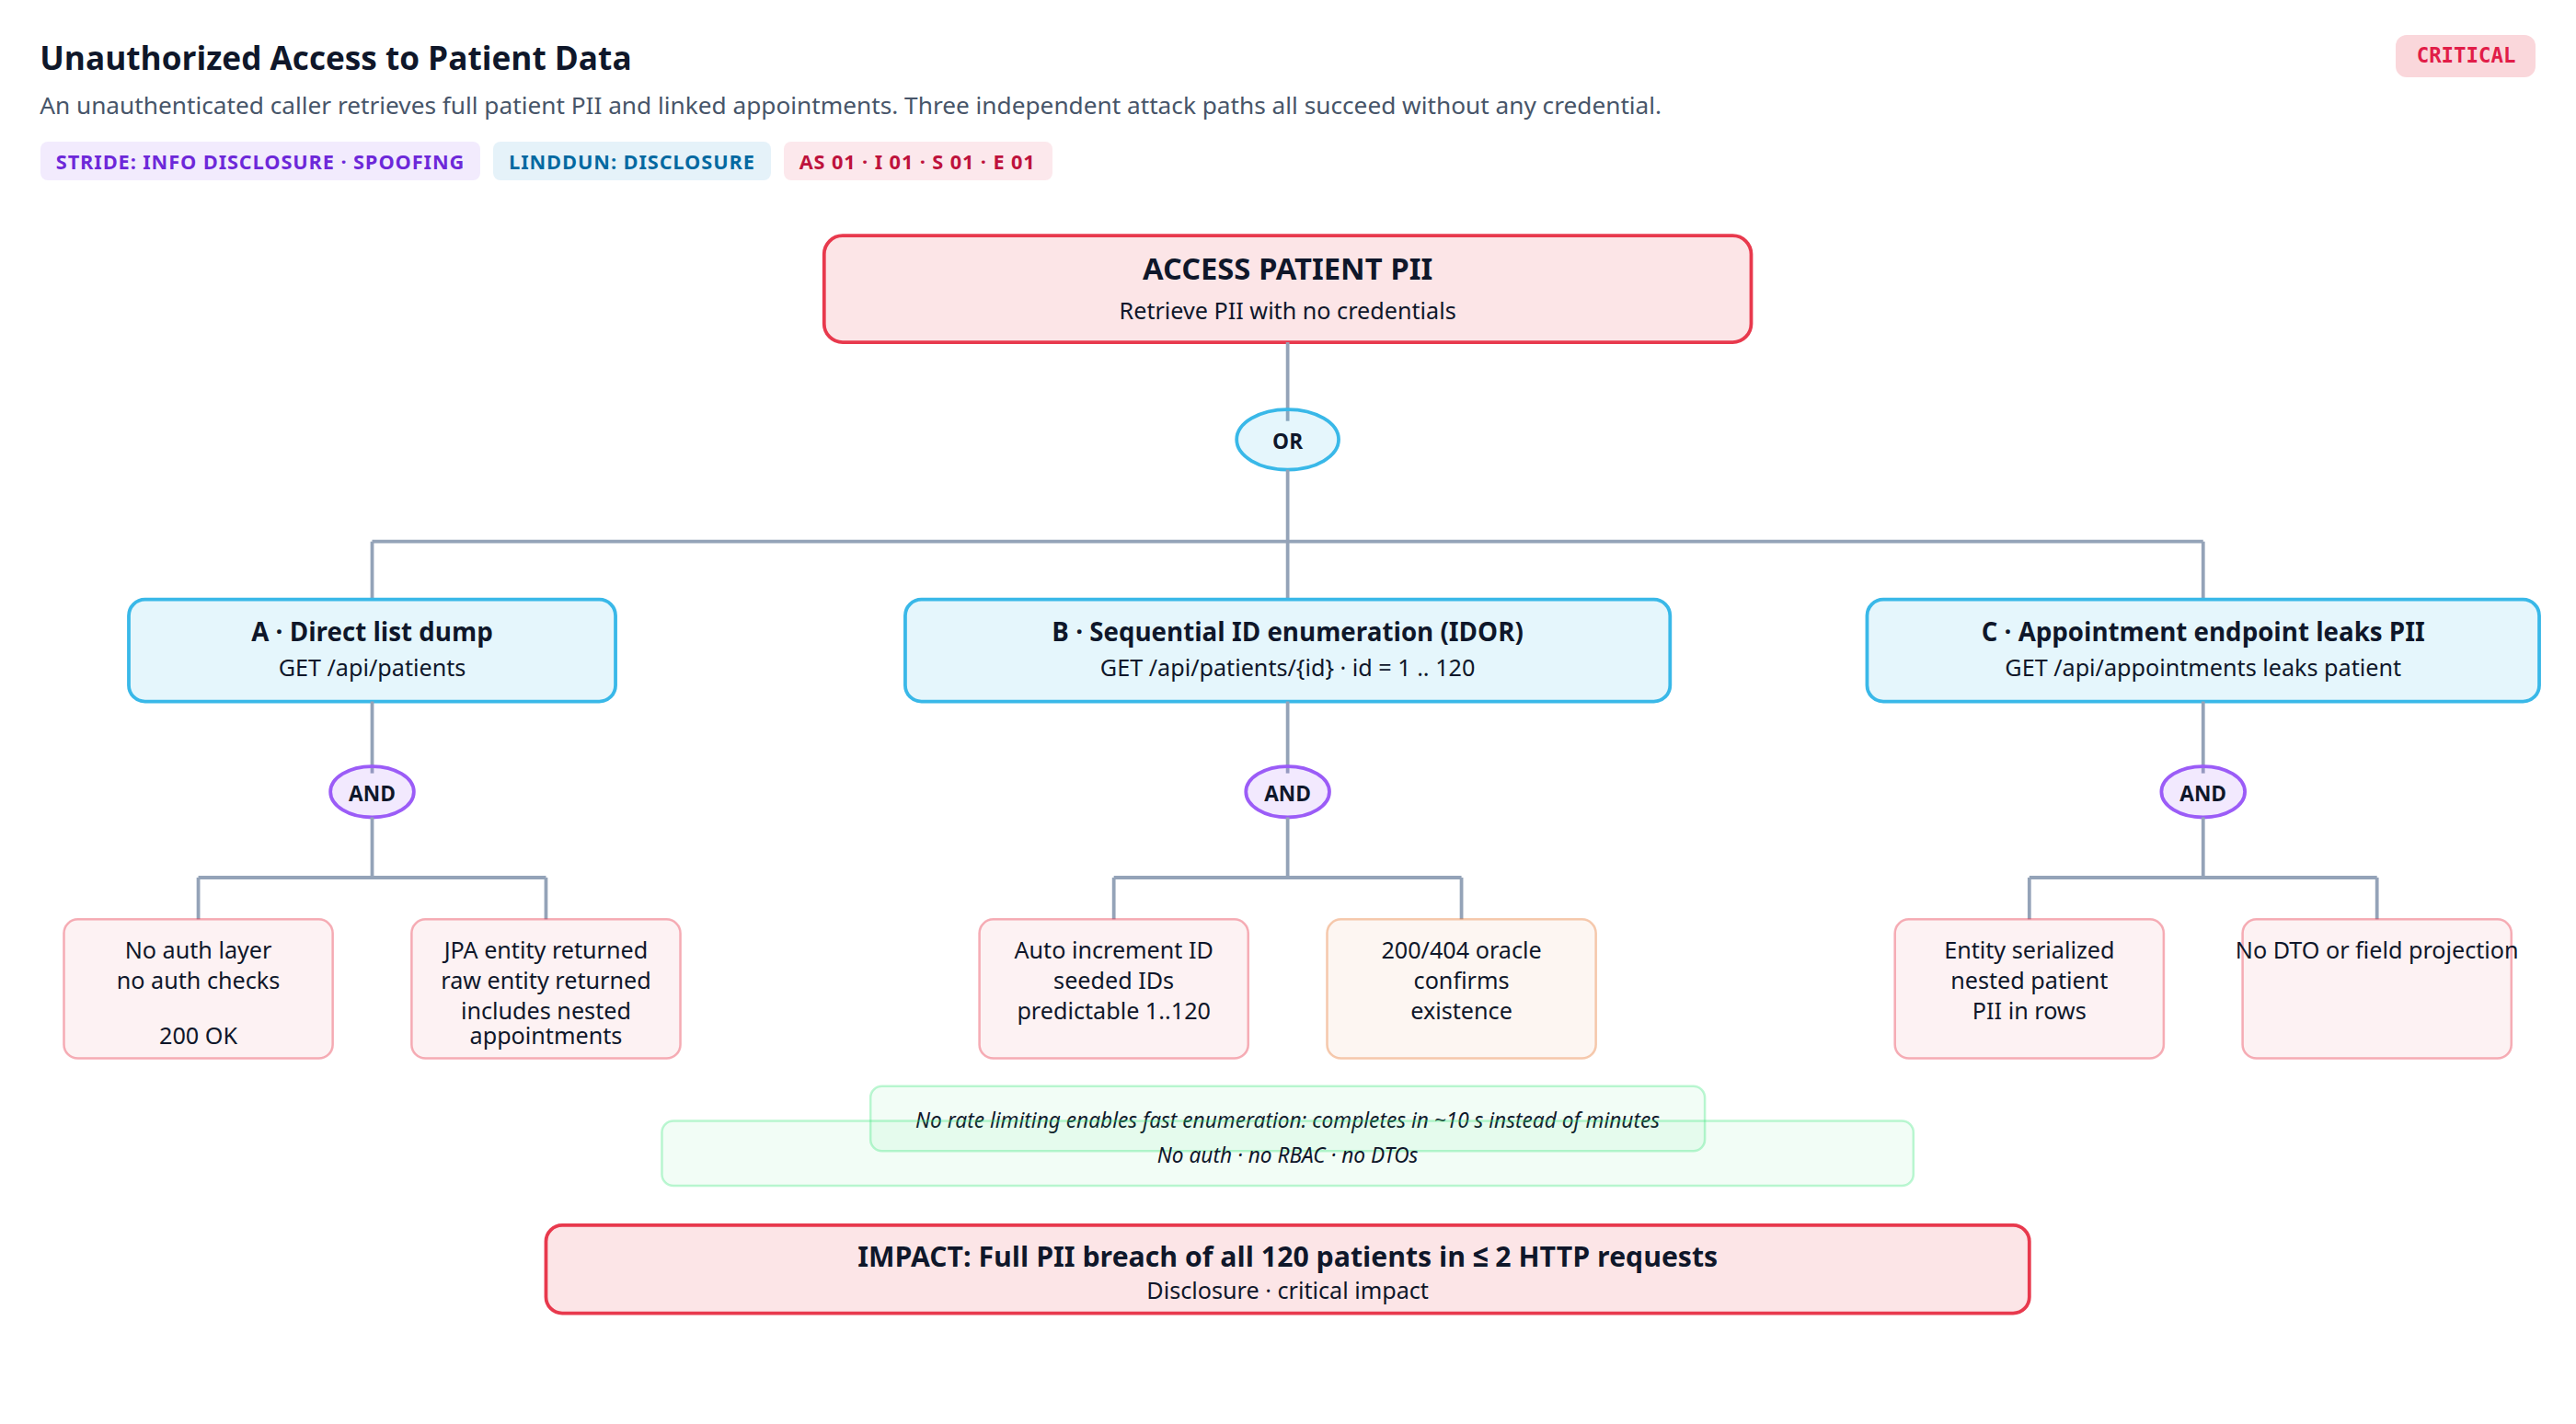
\includegraphics[width=0.92\linewidth]{01_unauthorized-data-access.png}
  \caption{Attack tree 1 -- Unauthorised Access to Patient Data}
\end{figure}

\begin{table}[H]
\centering
\begin{tabularx}{\linewidth}{l X}
\toprule
\textbf{Title}         & Unauthorised Access to Patient Data \\
\textbf{Description}   & An unauthenticated caller retrieves full patient PII and linked appointments. Three independent attack paths all succeed without any credential. \\
\textbf{STRIDE}        & Information Disclosure, Spoofing \\
\textbf{LINDDUN}       & Disclosure \\
\textbf{Abuse Stories} & AS-01, I-01, S-01, E-01 \\
\textbf{Severity}      & \critical \\
\bottomrule
\end{tabularx}
\end{table}

% ─── Tree 2 ──────────────────────────────────────────────────────────────────
\subsection*{2. Link Patient Identity to Health Patterns (AS-02 / AS-04)}

\begin{figure}[H]
  \centering
  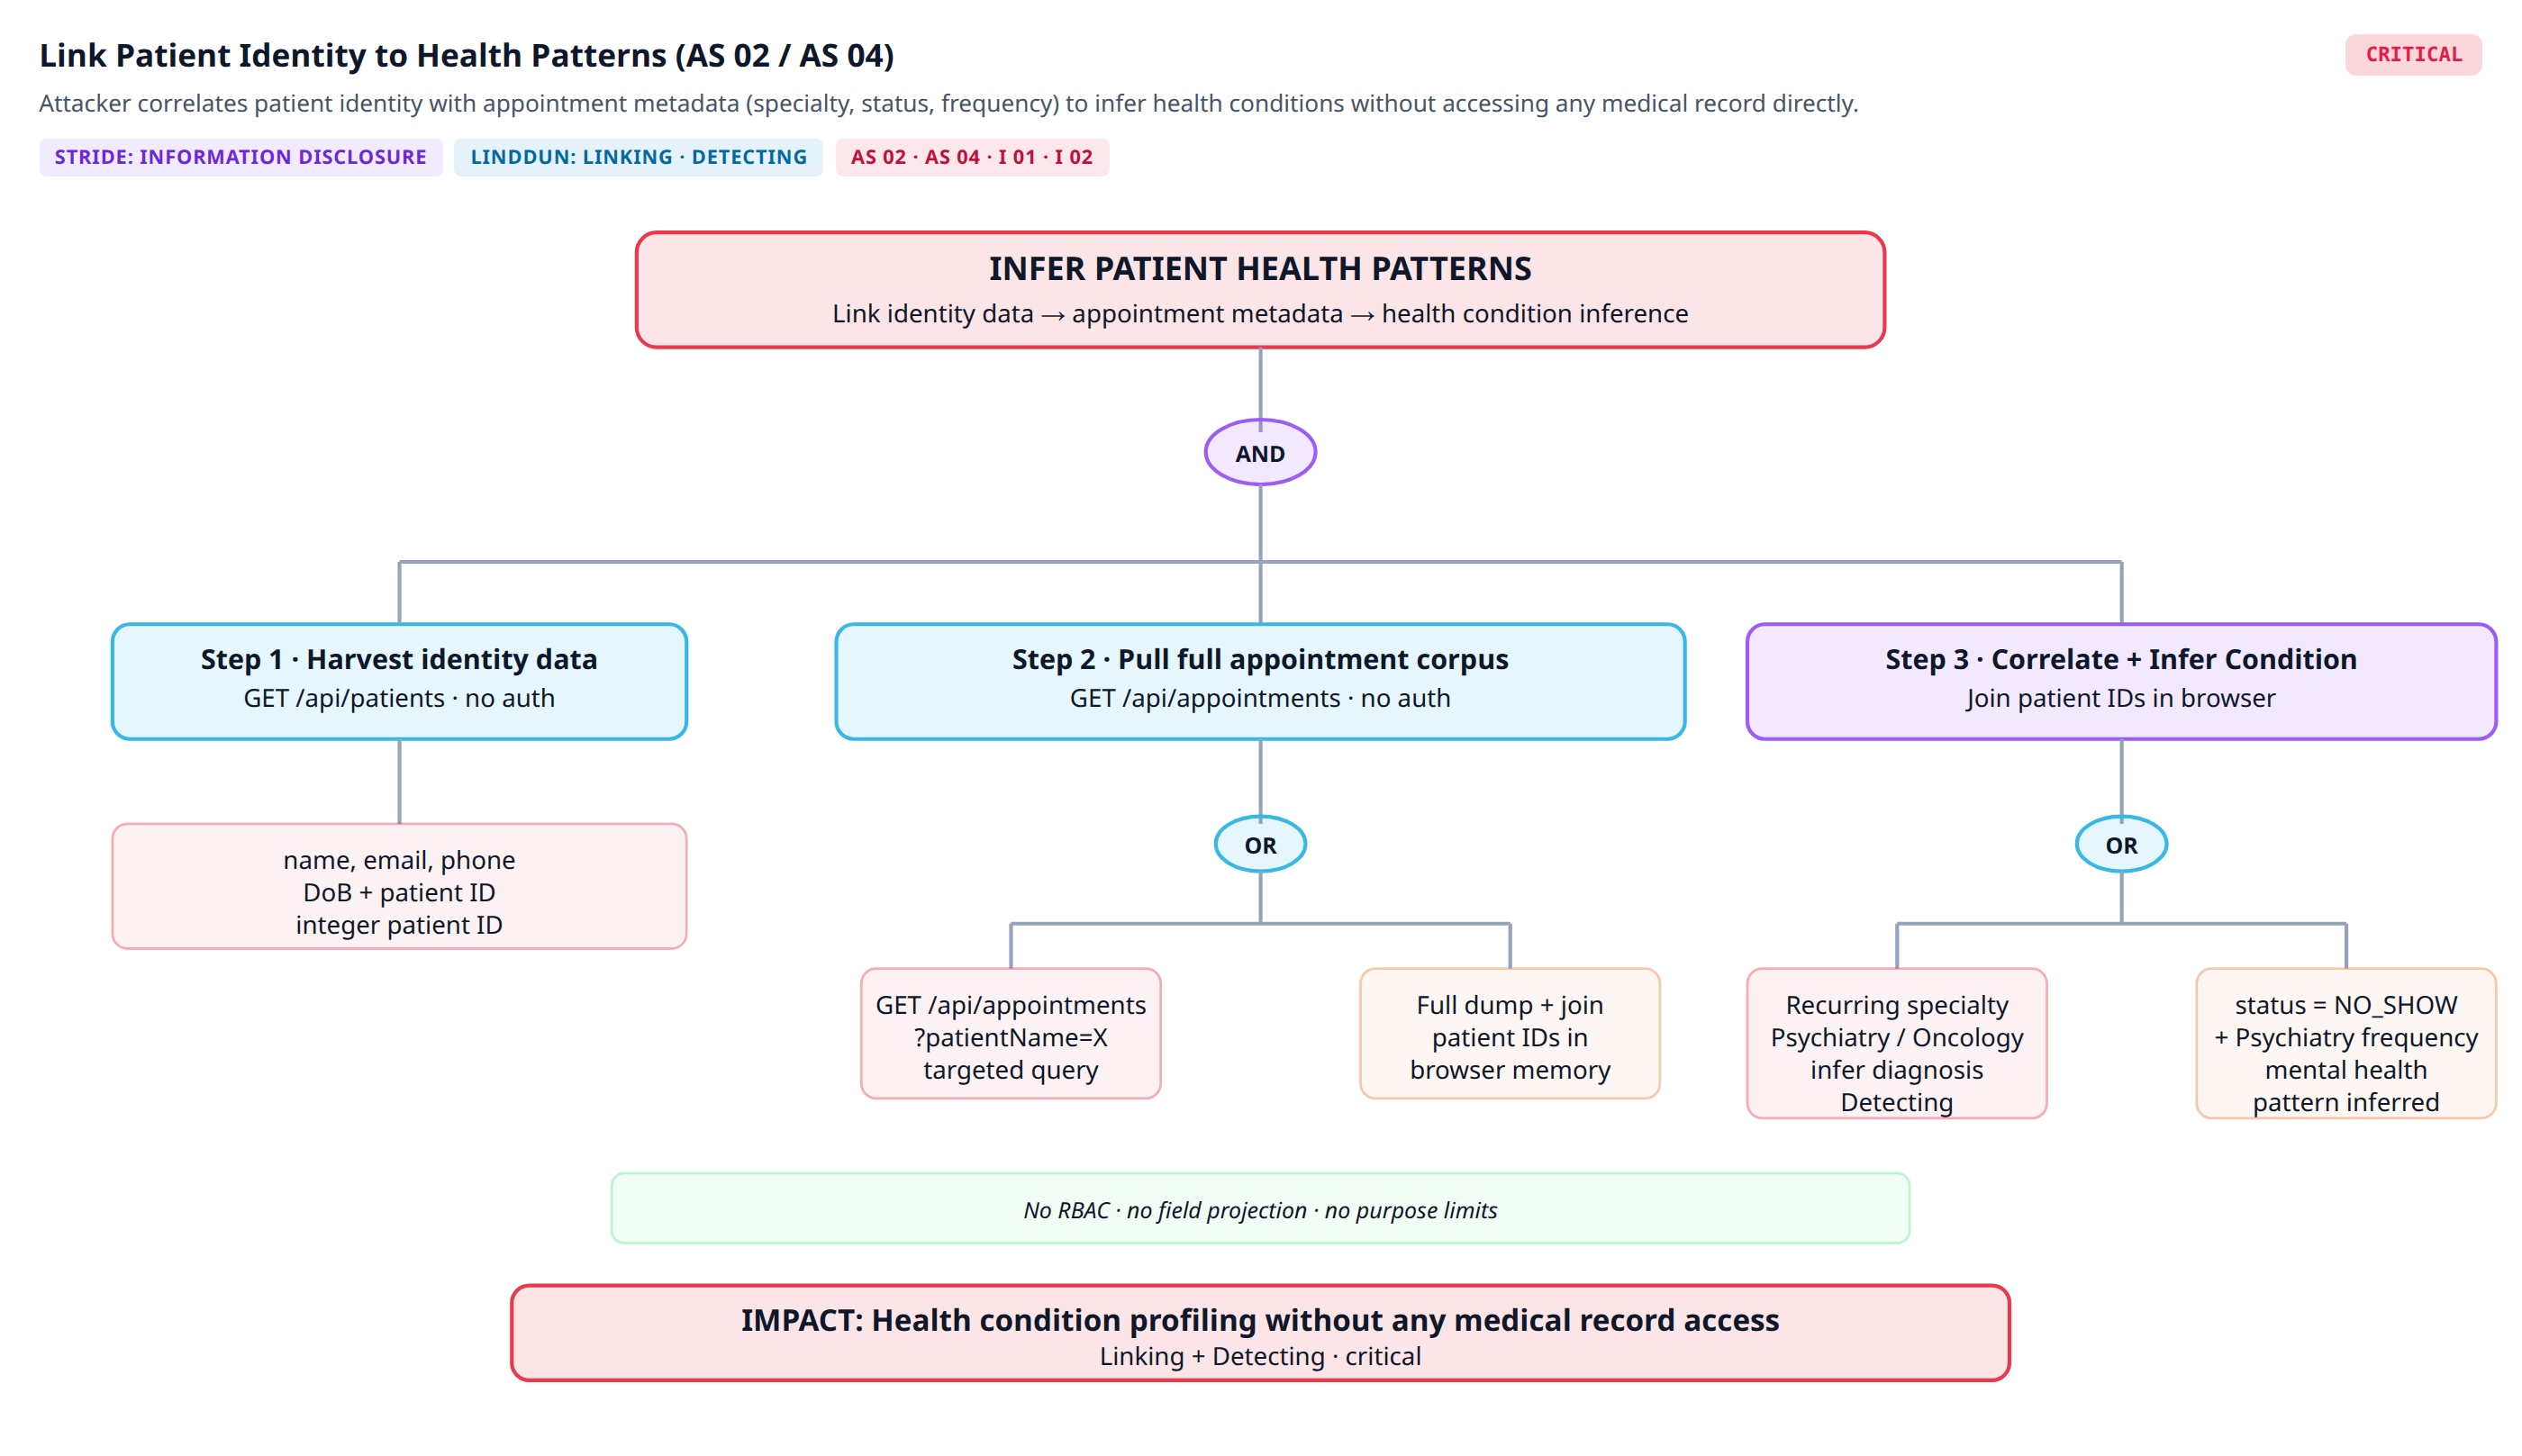
\includegraphics[width=0.92\linewidth]{02_linking-and-inference.png}
  \caption{Attack tree 2 -- Link Patient Identity to Health Patterns}
\end{figure}

\begin{table}[H]
\centering
\begin{tabularx}{\linewidth}{l X}
\toprule
\textbf{Title}         & Link Patient Identity to Health Patterns \\
\textbf{Description}   & Attacker correlates patient identity with appointment metadata (specialty, status, frequency) to infer health conditions without accessing any medical record directly. \\
\textbf{STRIDE}        & Information Disclosure \\
\textbf{LINDDUN}       & Linking, Detecting \\
\textbf{Abuse Stories} & AS-02, AS-04, I-01, I-02 \\
\textbf{Severity}      & \critical \\
\bottomrule
\end{tabularx}
\end{table}

% ─── Tree 3 ──────────────────────────────────────────────────────────────────
\subsection*{3. Direct Patient Identification via IDOR (AS-03)}

\begin{figure}[H]
  \centering
  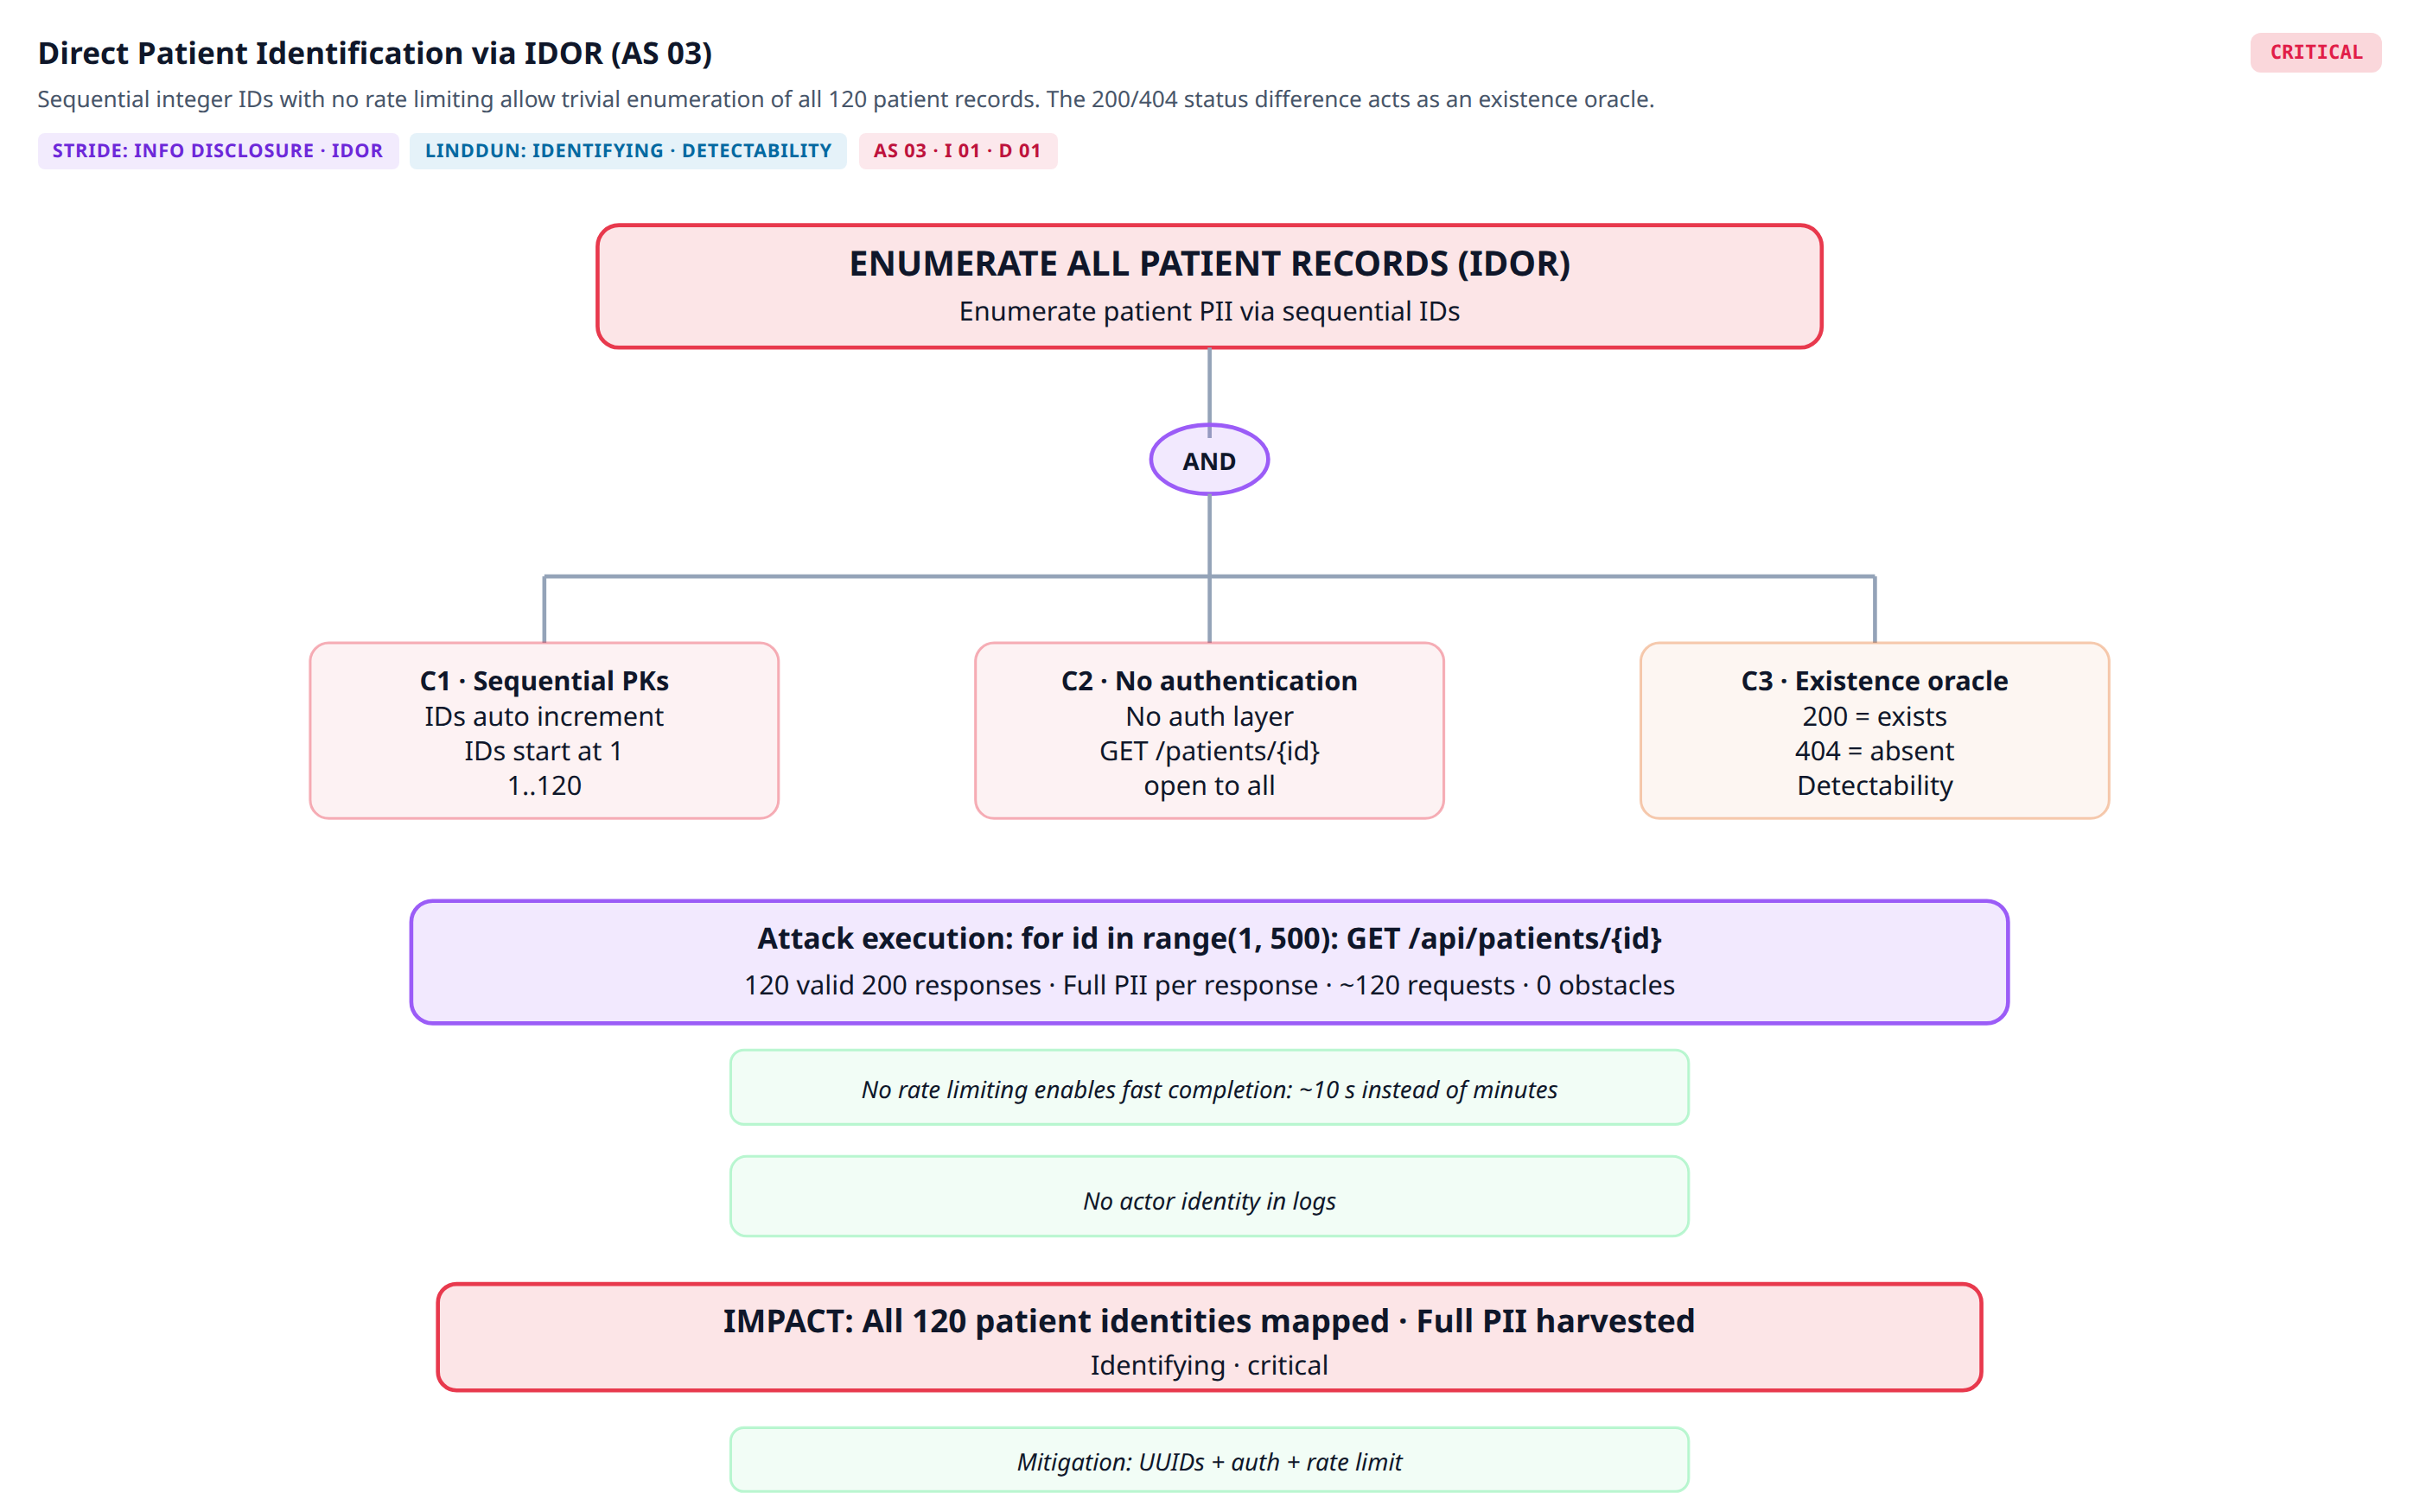
\includegraphics[width=0.85\linewidth]{03_patient-enumeration.png}
  \caption{Attack tree 3 -- Direct Patient Identification via IDOR}
\end{figure}

\begin{table}[H]
\centering
\begin{tabularx}{\linewidth}{l X}
\toprule
\textbf{Title}         & Direct Patient Identification via IDOR \\
\textbf{Description}   & Sequential integer IDs with no rate limiting allow trivial enumeration of all 120 patient records. The 200/404 status difference acts as an existence oracle. \\
\textbf{STRIDE}        & Information Disclosure, IDOR \\
\textbf{LINDDUN}       & Identifying, Detectability \\
\textbf{Abuse Stories} & AS-03, I-01, D-01 \\
\textbf{Severity}      & \critical \\
\bottomrule
\end{tabularx}
\end{table}

% ─── Tree 4 ──────────────────────────────────────────────────────────────────
\subsection*{4. Modify or Reassign Appointment Records (AS-05)}

\begin{figure}[H]
  \centering
  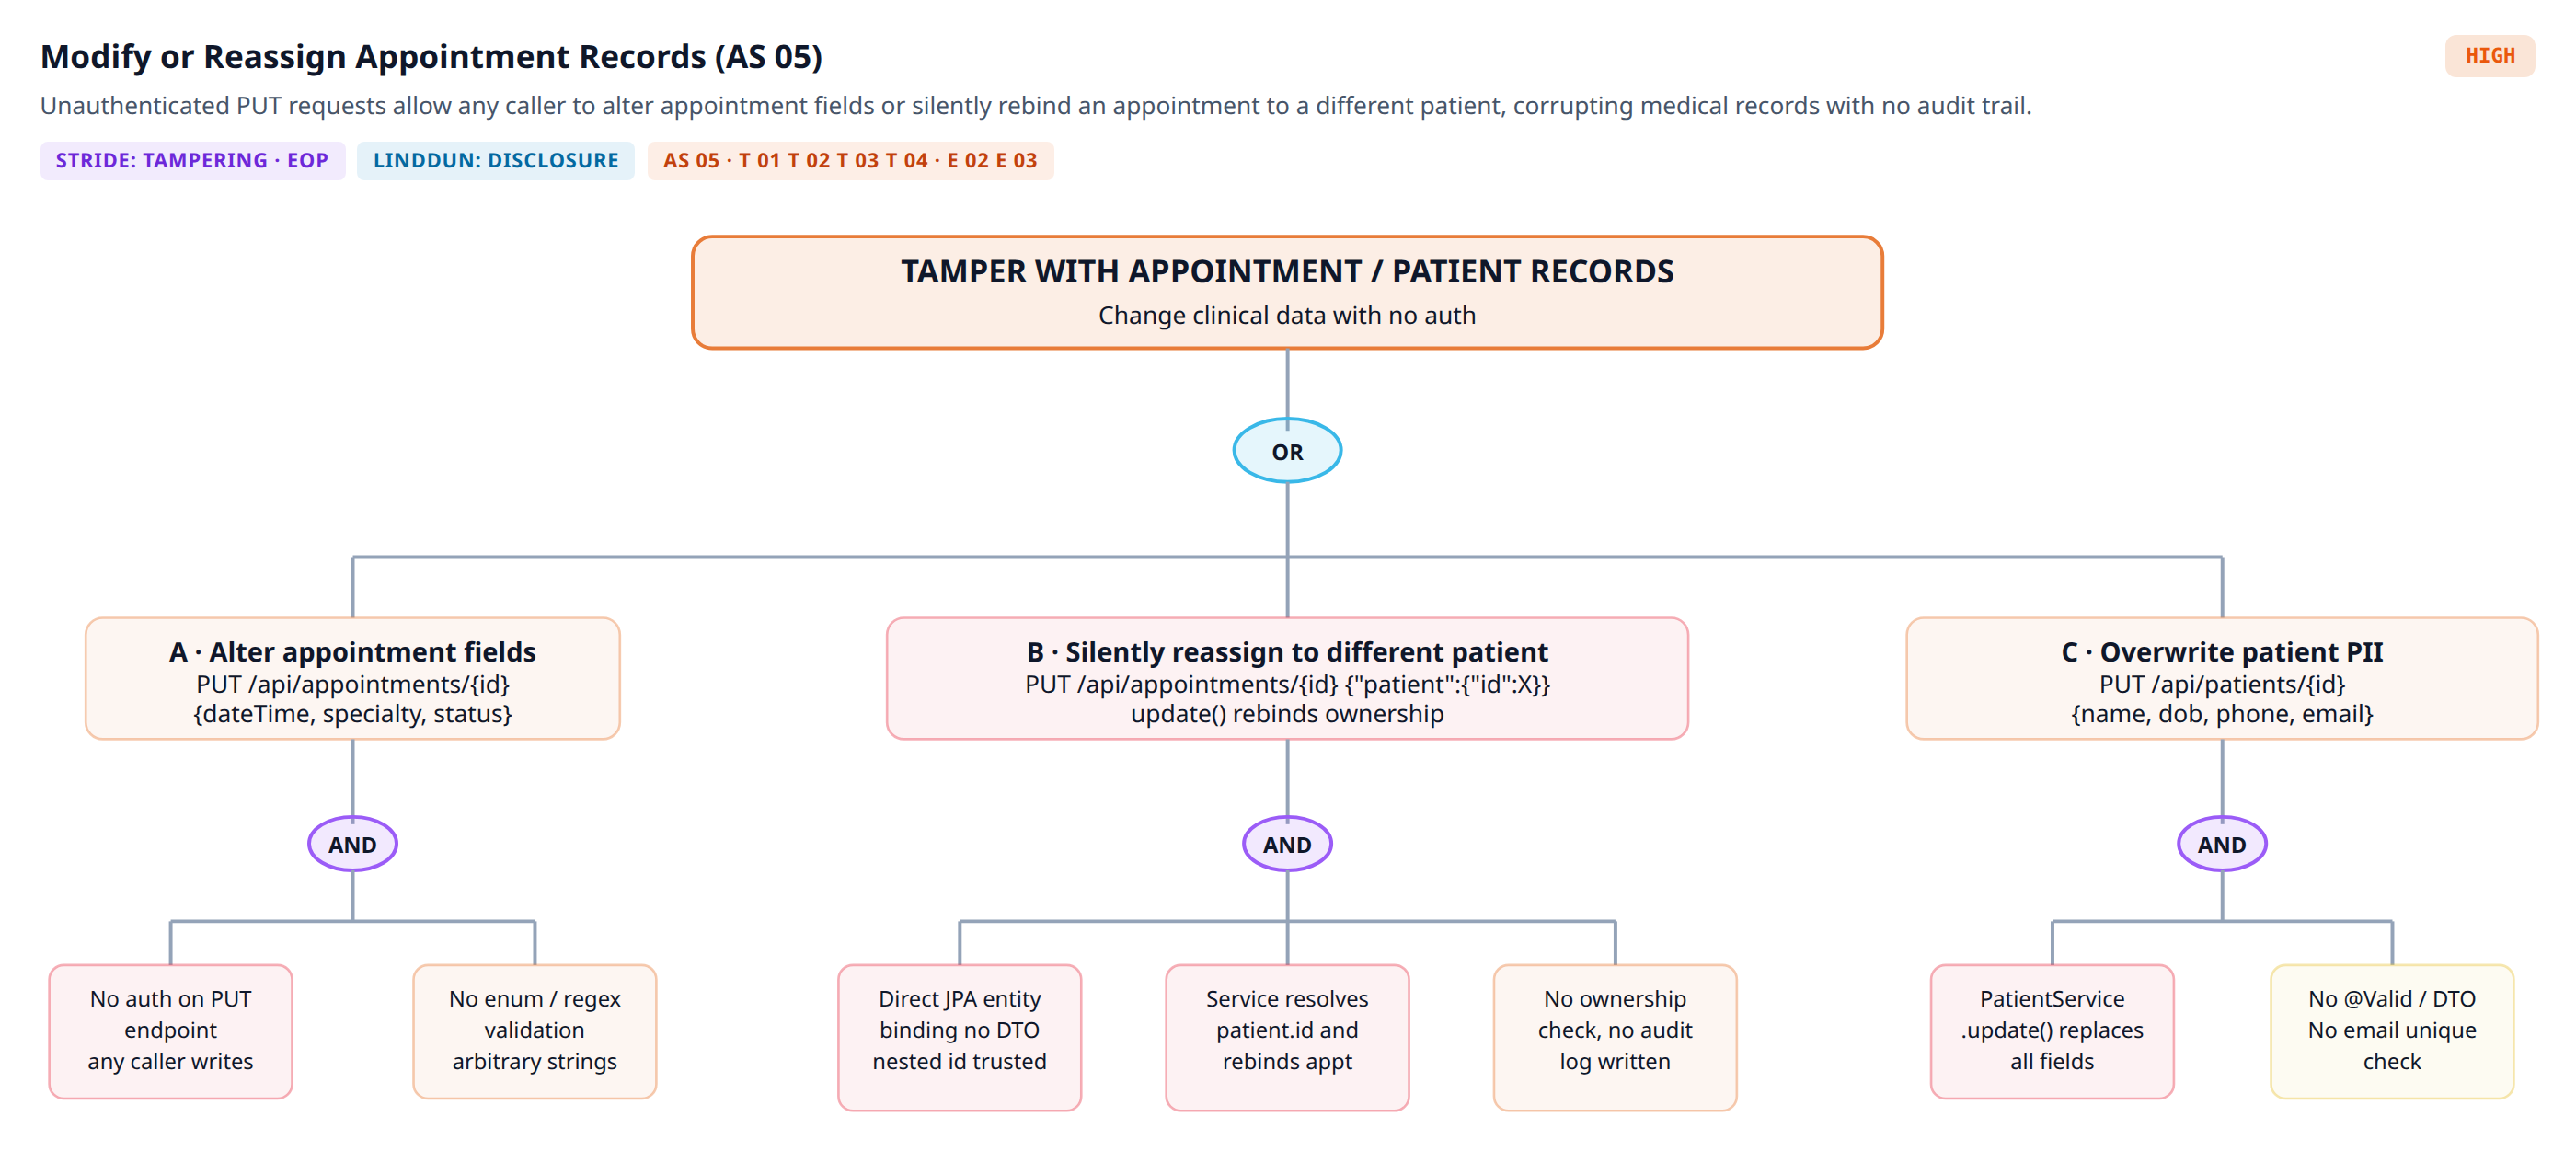
\includegraphics[width=\linewidth]{04_record-tampering.png}
  \caption{Attack tree 4 -- Modify or Reassign Appointment Records}
\end{figure}

\begin{table}[H]
\centering
\begin{tabularx}{\linewidth}{l X}
\toprule
\textbf{Title}         & Modify or Reassign Appointment Records \\
\textbf{Description}   & Unauthenticated PUT requests allow any caller to alter appointment fields or silently rebind an appointment to a different patient, corrupting medical records with no audit trail. \\
\textbf{STRIDE}        & Tampering, Elevation of Privilege \\
\textbf{LINDDUN}       & Disclosure \\
\textbf{Abuse Stories} & AS-05, T-01--T-04, E-02, E-03 \\
\textbf{Severity}      & \high \\
\bottomrule
\end{tabularx}
\end{table}

% ─── Tree 5 ──────────────────────────────────────────────────────────────────
\subsection*{5. Destroy Patient Records via Cascade Deletion (AS-06)}

\begin{figure}[H]
  \centering
  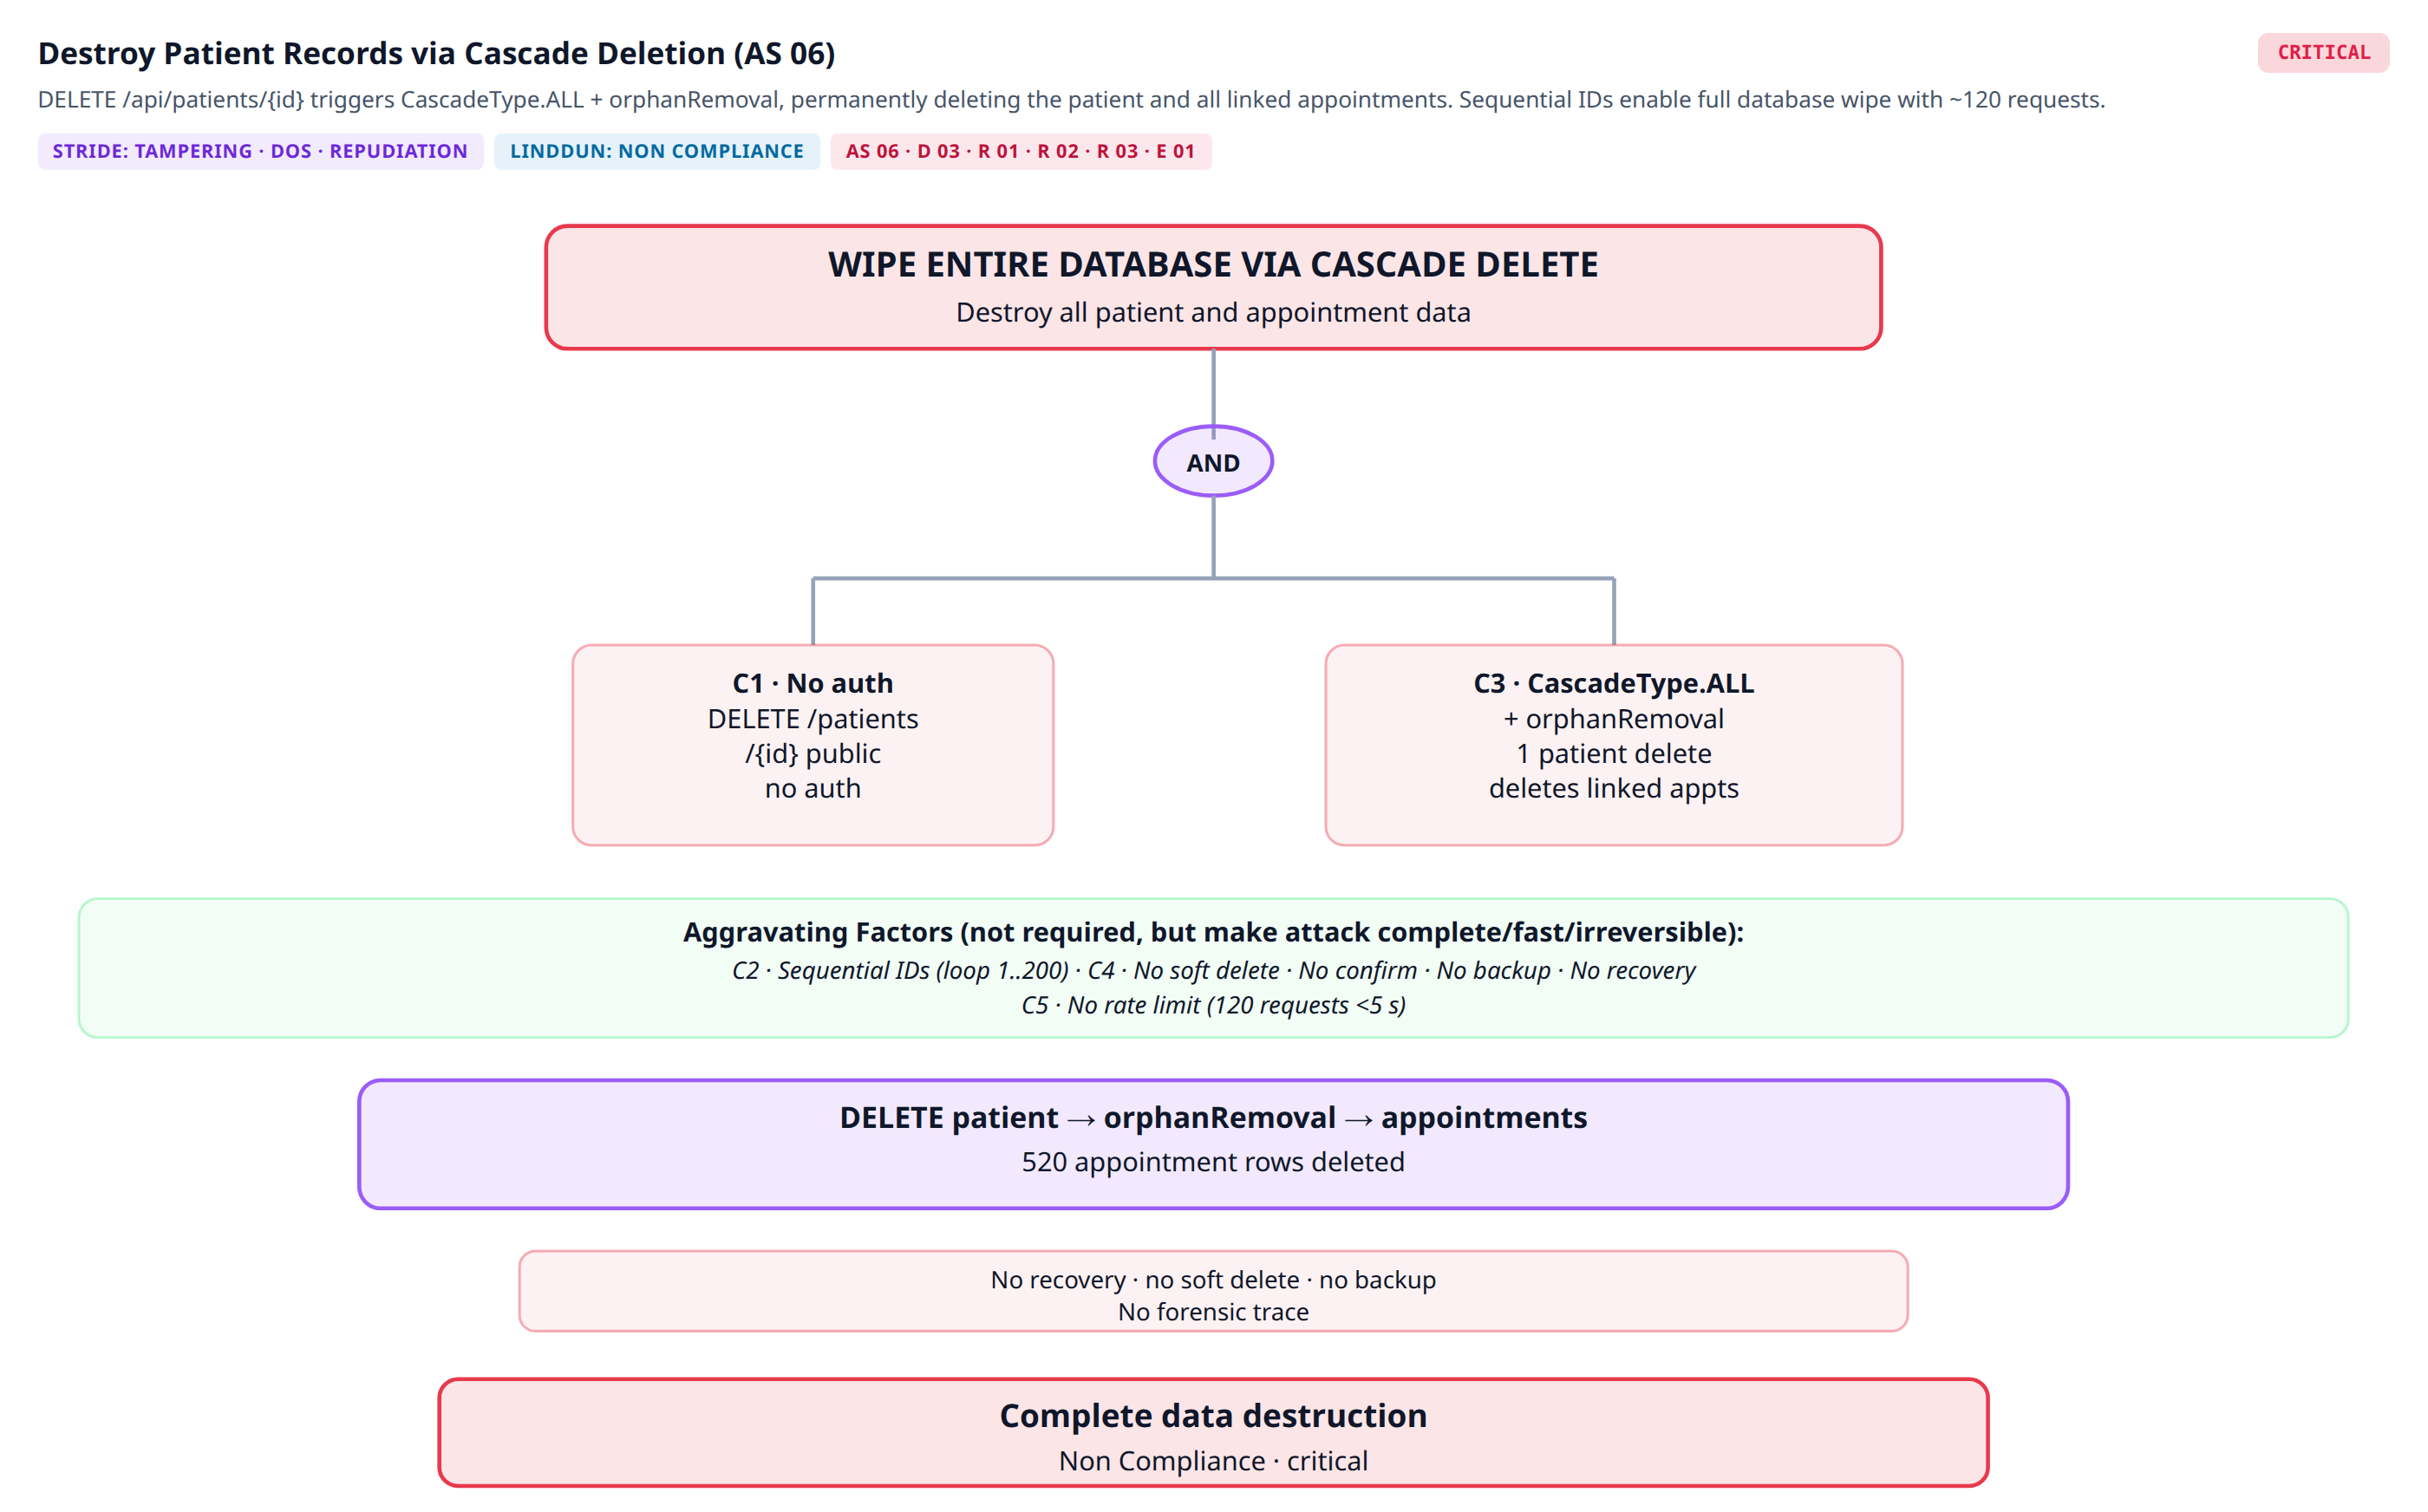
\includegraphics[width=\linewidth]{05_cascade-deletion.png}
  \caption{Attack tree 5 -- Destroy Patient Records via Cascade Deletion}
\end{figure}

\begin{table}[H]
\centering
\begin{tabularx}{\linewidth}{l X}
\toprule
\textbf{Title}         & Destroy Patient Records via Cascade Deletion \\
\textbf{Description}   & \texttt{DELETE /api/patients/\{id\}} triggers CascadeType.ALL + orphanRemoval, permanently deleting the patient and all linked appointments. Sequential IDs enable a full database wipe with $\sim$120 requests. \\
\textbf{STRIDE}        & Tampering, DoS, Repudiation \\
\textbf{LINDDUN}       & Non-Compliance \\
\textbf{Abuse Stories} & AS-06, D-03, R-01, R-02, R-03, E-01 \\
\textbf{Severity}      & \critical \\
\bottomrule
\end{tabularx}
\end{table}

% ─── Tree 6 ──────────────────────────────────────────────────────────────────
\subsection*{6. Perform Undetectable Actions (AS-07)}

\begin{figure}[H]
  \centering
  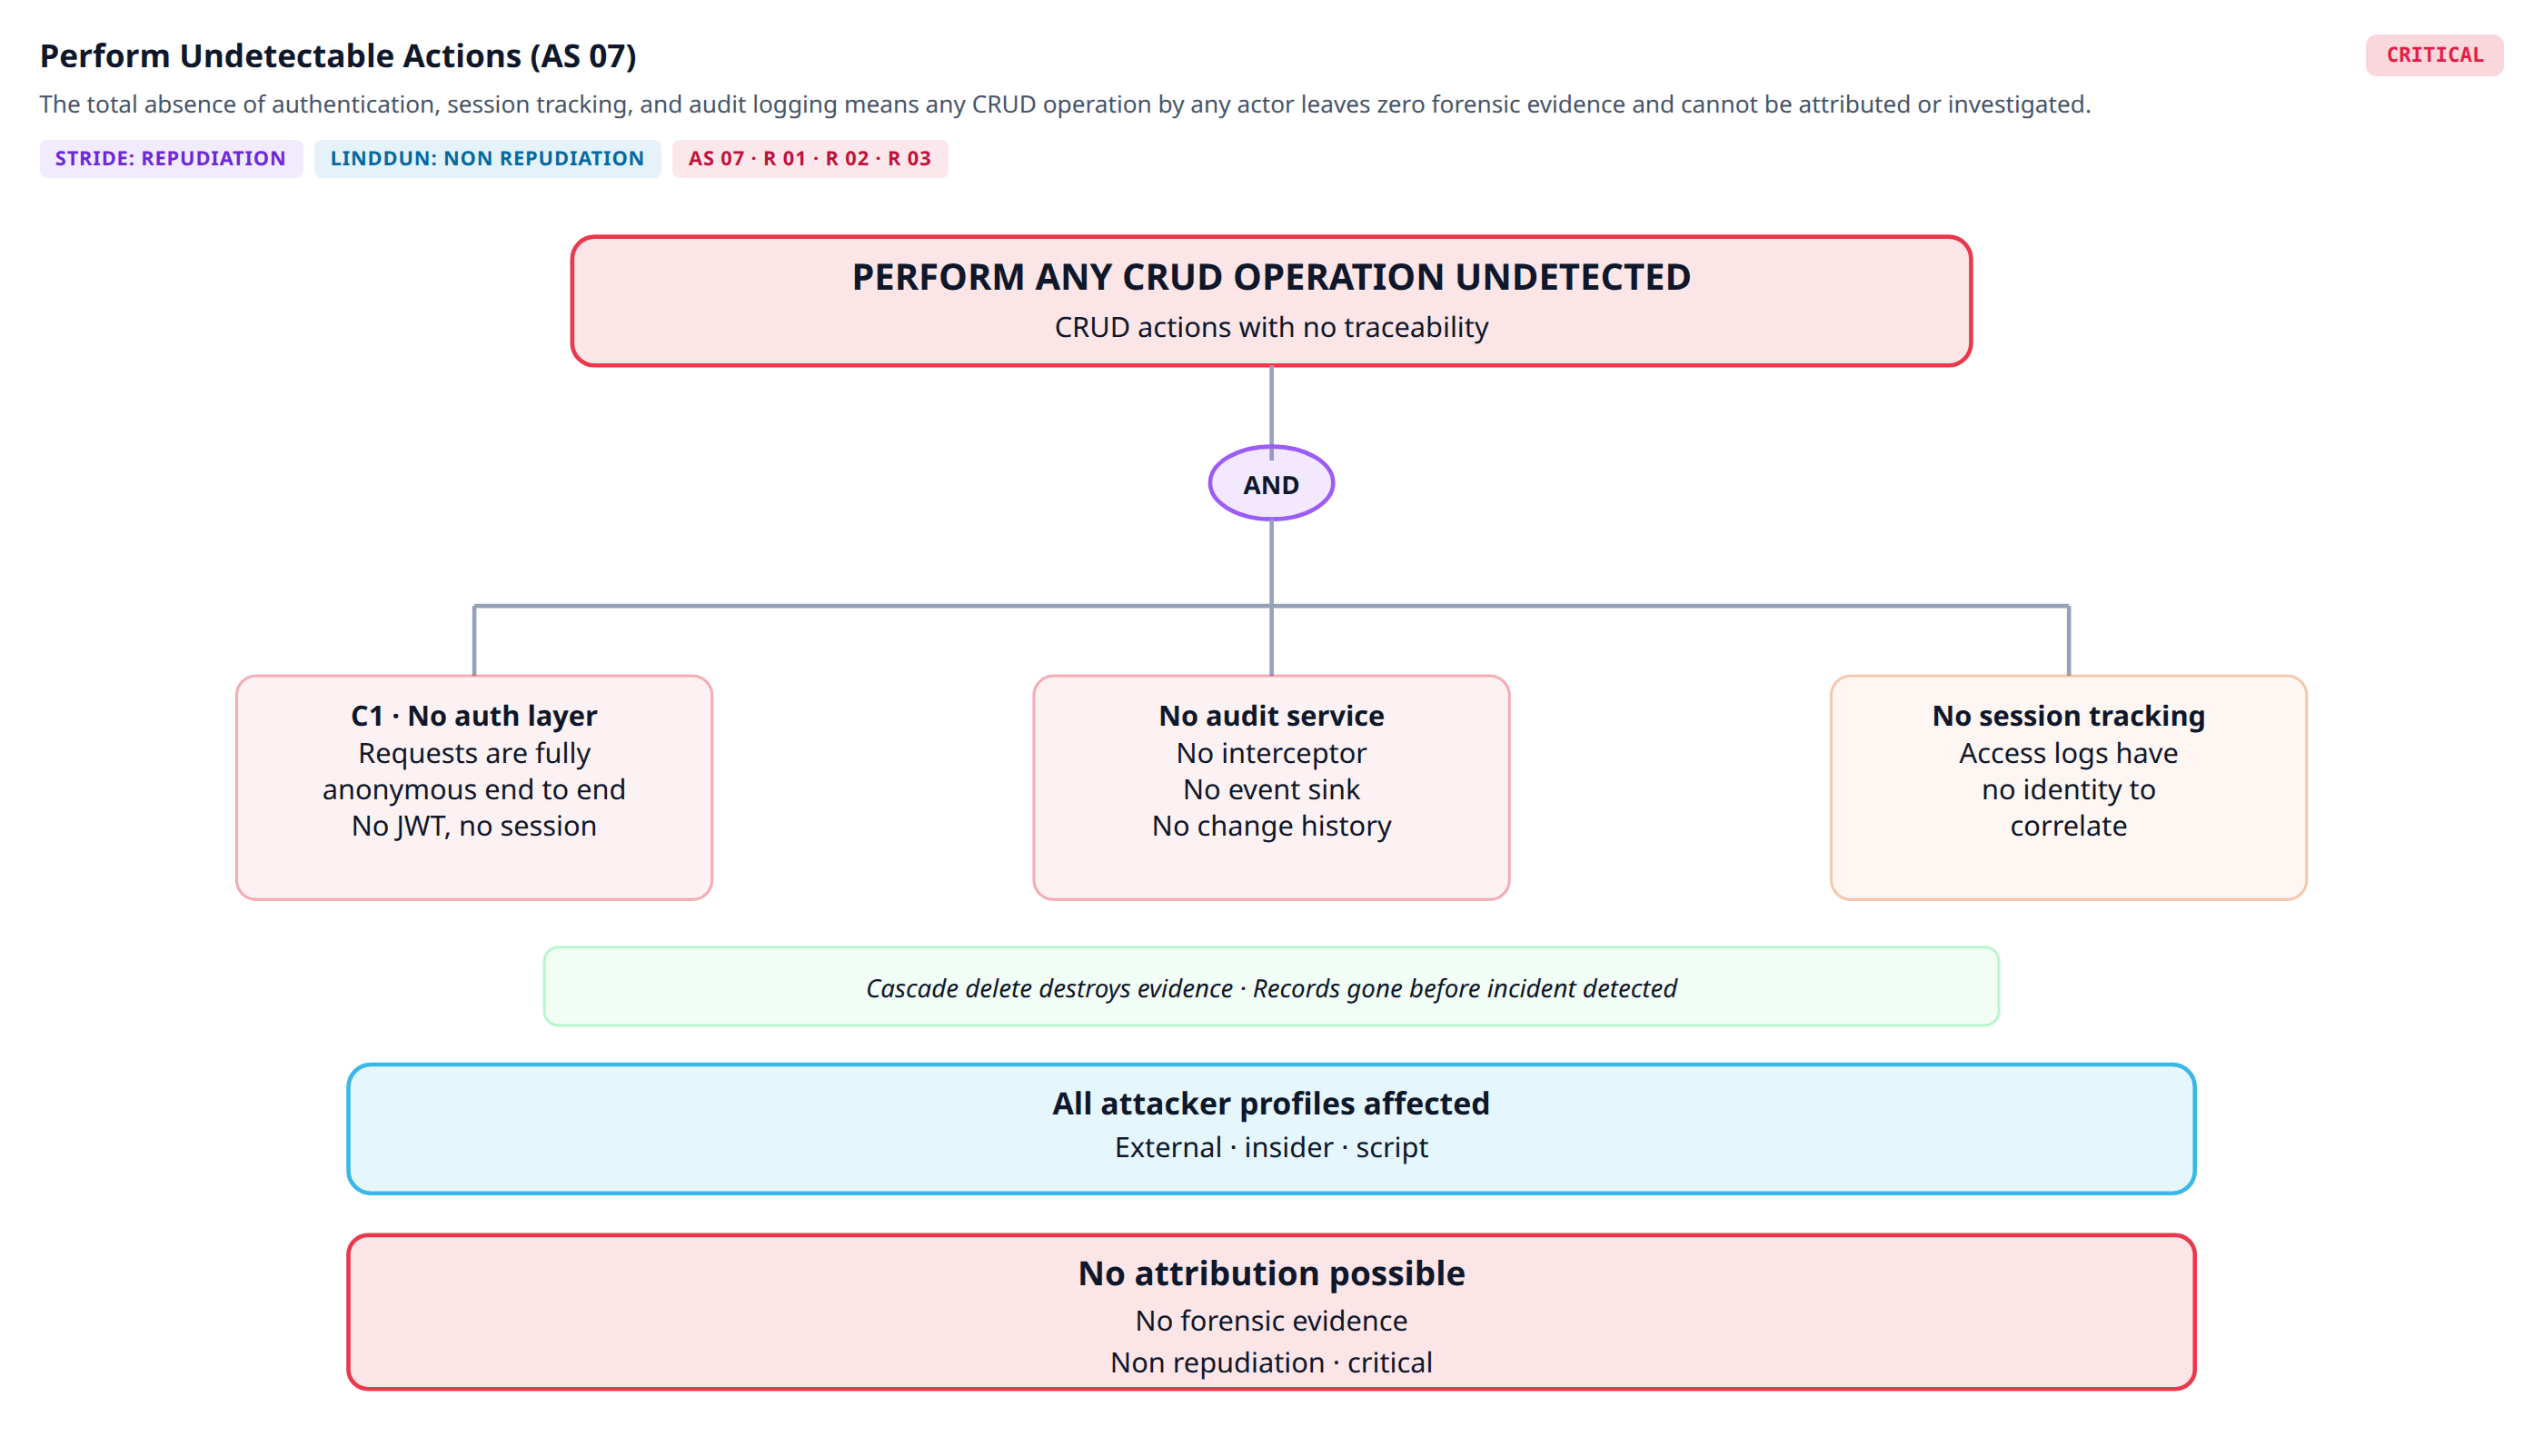
\includegraphics[width=\linewidth]{06_undetectable-actions.png}
  \caption{Attack tree 6 -- Perform Undetectable Actions}
\end{figure}

\begin{table}[H]
\centering
\begin{tabularx}{\linewidth}{l X}
\toprule
\textbf{Title}         & Perform Undetectable Actions \\
\textbf{Description}   & The total absence of authentication, session tracking, and audit logging means any CRUD operation leaves zero forensic evidence and cannot be attributed or investigated. \\
\textbf{STRIDE}        & Repudiation \\
\textbf{LINDDUN}       & Non-repudiation \\
\textbf{Abuse Stories} & AS-07, R-01, R-02, R-03 \\
\textbf{Severity}      & \critical \\
\bottomrule
\end{tabularx}
\end{table}

% ─── Tree 7 ──────────────────────────────────────────────────────────────────
\subsection*{7. Overload API / Denial of Service (AS-08)}

\begin{figure}[H]
  \centering
  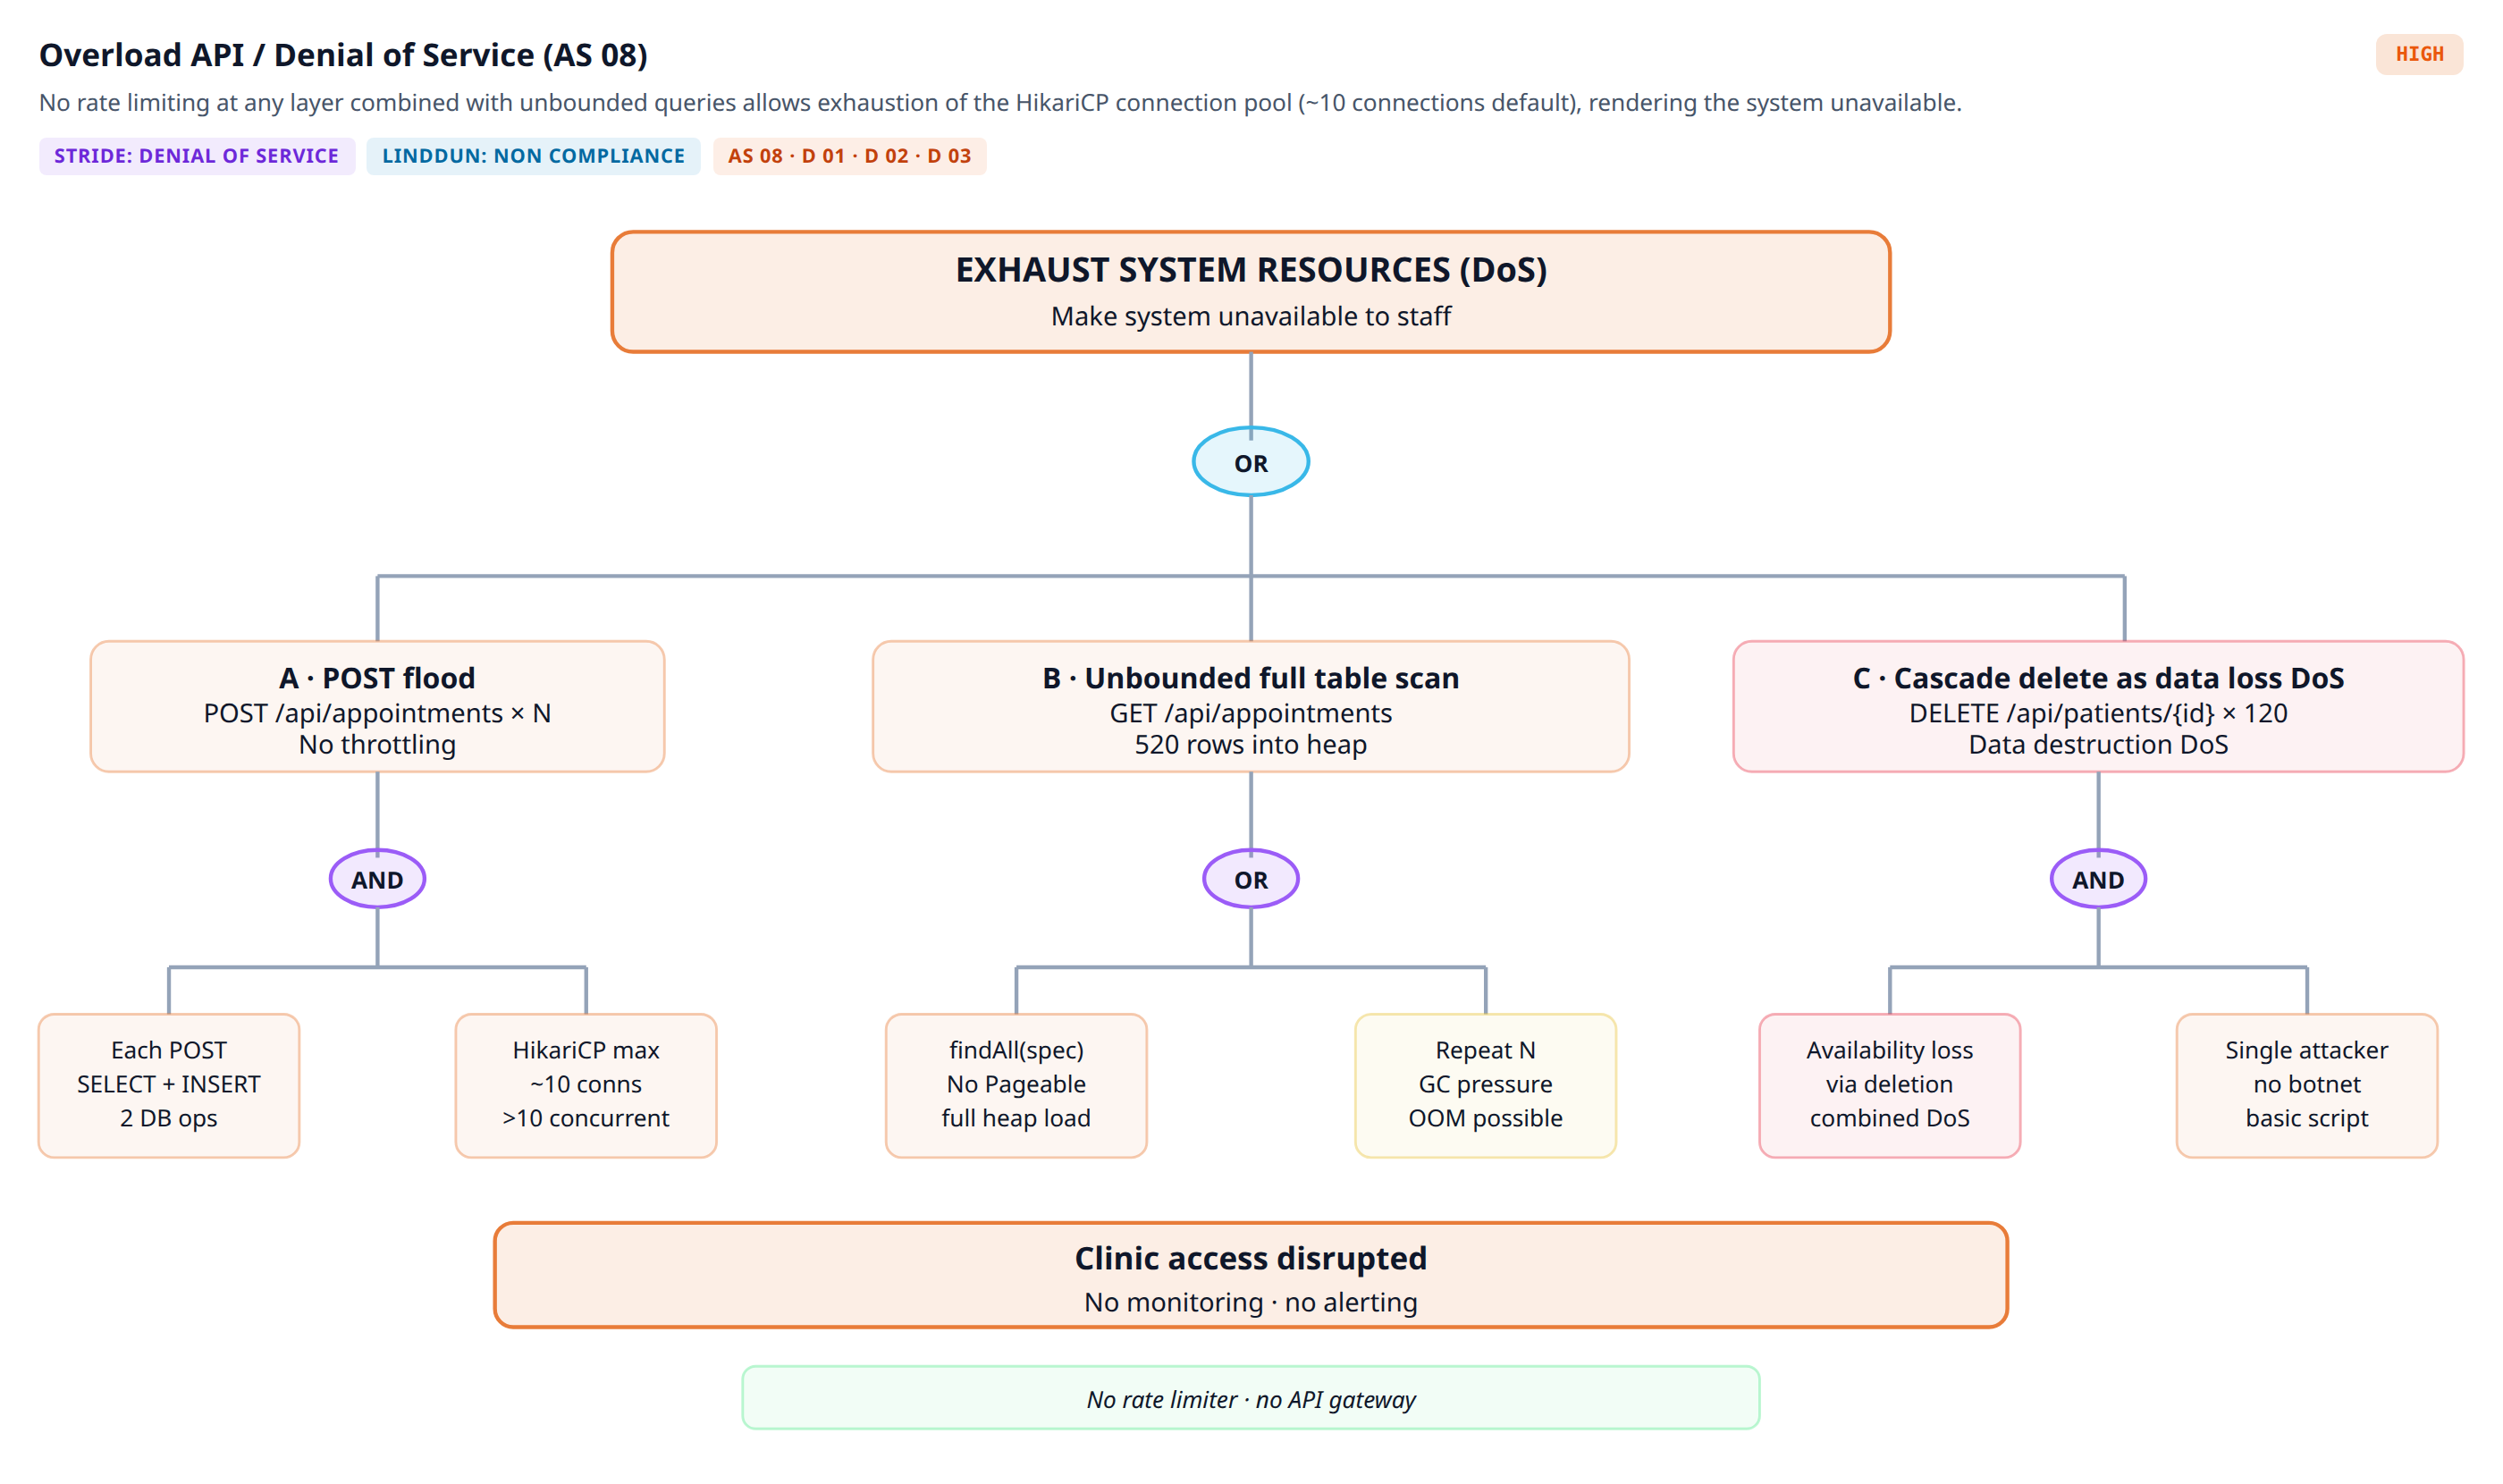
\includegraphics[width=\linewidth]{07_api-overload.png}
  \caption{Attack tree 7 -- Overload API / Denial of Service}
\end{figure}

\begin{table}[H]
\centering
\begin{tabularx}{\linewidth}{l X}
\toprule
\textbf{Title}         & Overload API / Denial of Service \\
\textbf{Description}   & No rate limiting at any layer combined with unbounded queries allows exhaustion of the HikariCP connection pool ($\sim$10 connections default), rendering the system unavailable. \\
\textbf{STRIDE}        & Denial of Service \\
\textbf{LINDDUN}       & Non-Compliance \\
\textbf{Abuse Stories} & AS-08, D-01, D-02, D-03 \\
\textbf{Severity}      & \high \\
\bottomrule
\end{tabularx}
\end{table}

% ══════════════════════════════════════════════════════════════════════════════
\chapter{SAST -- Static Application Security Testing}
% ══════════════════════════════════════════════════════════════════════════════

Static Application Security Testing (SAST) was used in this project to analyse source code, security configuration, and build artefacts without relying on runtime exploitation. Its purpose is to identify insecure coding patterns, exposed secrets, vulnerable dependencies, and insecure project configurations as early as possible in the development lifecycle.

For this project, SAST is organised as a three-level process:
\begin{itemize}
  \item \textbf{pre-commit} -- fast local feedback before code is committed;
  \item \textbf{pull request} -- gated review before changes are merged;
  \item \textbf{nightly} -- broader recurring analysis with deeper coverage.
\end{itemize}

% ─────────────────────────────────────────────────────────────────────────────
\section{Objectives}
% ─────────────────────────────────────────────────────────────────────────────

\begin{itemize}
  \item Detect insecure code patterns in the Java Spring Boot backend and React/Vite frontend.
  \item Identify secrets, dependency risks, and misconfigurations before deployment.
  \item Prevent obvious security issues from reaching the main branch.
  \item Provide evidence through GitHub Actions runs, uploaded artefacts, and summary reports.
  \item Support the wider application security assessment together with DAST and manual pentesting.
\end{itemize}

% ─────────────────────────────────────────────────────────────────────────────
\section{Scope}
% ─────────────────────────────────────────────────────────────────────────────

The static analysis scope covers the backend source code in \texttt{src/backend}, the frontend source code in \texttt{src/frontend}, the repository-level security configuration, the GitHub Actions workflow logic, and Docker-related build artefacts.

% ─────────────────────────────────────────────────────────────────────────────
\section{Three-Level SAST Strategy}
% ─────────────────────────────────────────────────────────────────────────────

\subsection{Pre-Commit Level}

Defined through \texttt{.pre-commit-config.yaml}. Uses:
\begin{itemize}
  \item \textbf{Gitleaks} -- detects secrets and sensitive tokens in staged changes.
  \item \textbf{Semgrep} -- fast security-focused scan using \texttt{p/security-audit} and custom rules in \texttt{.github/config/security/semgrep.yml}.
\end{itemize}

This level is intentionally lightweight and optimised for quick developer feedback.

\subsection{Pull Request Level}

Runs on pull requests through \texttt{sast.yml}. Performs:
\begin{itemize}
  \item \textbf{Gitleaks} -- over the Git range introduced by the PR.
  \item \textbf{Semgrep} -- enforcing scan for ERROR findings; advisory for WARNING and INFO.
  \item \textbf{ESLint Security} -- frontend-oriented security linting.
  \item \textbf{Trivy} -- filesystem and backend dependency scans.
  \item \textbf{SonarQube} -- with a project-specific quality gate.
\end{itemize}

\textbf{SonarQube quality gate rules:}
\begin{itemize}
  \item No new bugs; no new vulnerabilities.
  \item All new security hotspots must be reviewed.
  \item No significant maintainability degradation in new code.
  \item Duplication in new code must stay below 3\%.
\end{itemize}

A \textbf{SAST Security Summary} is posted back to the pull request.

\subsection{Nightly Level}

Runs through \texttt{sast-nightly.yml}. Performs:
\begin{itemize}
  \item \textbf{CodeQL} -- for Java/Kotlin and JavaScript/TypeScript.
  \item \textbf{Semgrep} -- broader rule sets: \texttt{p/owasp-top-ten}, \texttt{p/java}, \texttt{p/javascript}, and custom rules.
  \item \textbf{Trivy} -- image scanning over the backend and frontend Docker images.
\end{itemize}

% ─────────────────────────────────────────────────────────────────────────────
\section{Why the Three Levels Matter}
% ─────────────────────────────────────────────────────────────────────────────

\begin{itemize}
  \item \textbf{pre-commit} minimises developer mistakes before code is pushed.
  \item \textbf{pull request} provides security gating and reviewer visibility before merge.
  \item \textbf{nightly} provides deeper scheduled assurance and broader long-term monitoring.
\end{itemize}

% ─────────────────────────────────────────────────────────────────────────────
\section{Strengths and Limitations}
% ─────────────────────────────────────────────────────────────────────────────

\textbf{Strengths:} Security checks are distributed across different development lifecycle moments rather than concentrated in a single scan. GitHub Actions artefacts, workflow logs, and generated summaries make results easier to review and present as evidence.

\textbf{Limitations:} Static analysis can produce false positives and some findings may not be exploitable in practice. The pre-commit layer also depends on developers having the tooling correctly installed locally. SAST alone cannot fully assess runtime behaviour or business logic flaws, so it should be seen as one component of a broader security assessment.

% ─────────────────────────────────────────────────────────────────────────────
\section{Results}
% ─────────────────────────────────────────────────────────────────────────────

\subsection{Pre-Commit Results}

The pre-commit hook was executed successfully via \texttt{pre-commit run --all-files}. Both Gitleaks and Semgrep passed with no blocking findings, confirming no secrets or high-severity patterns in the staged codebase.

\begin{figure}[H]
  \centering
  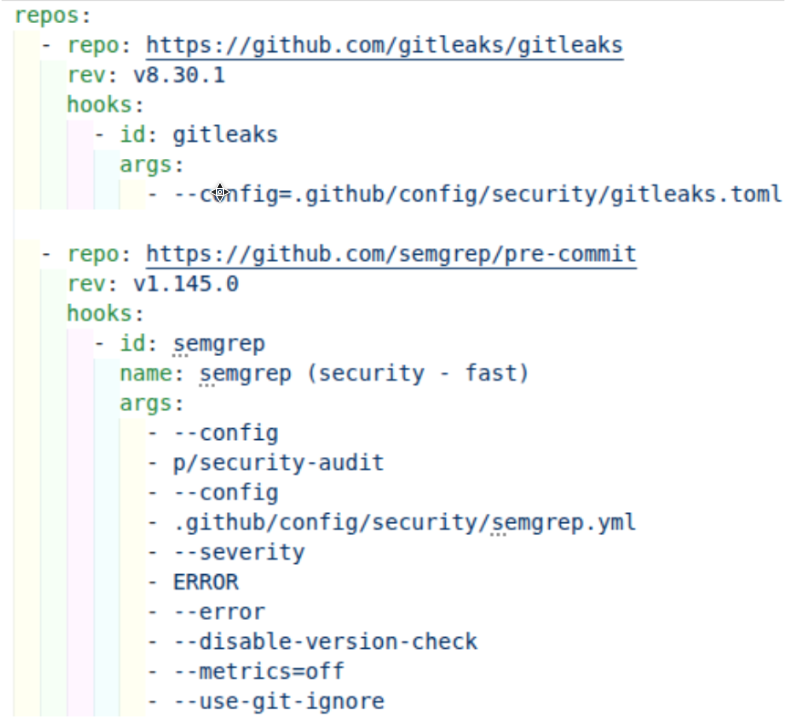
\includegraphics[width=0.80\linewidth]{precommit_config.png}
  \caption{Pre-commit hook configuration (\texttt{.pre-commit-config.yaml}) -- Gitleaks v8.30.1 and Semgrep v1.145.0}
\end{figure}

\subsection{Pull Request Results}

\begin{table}[H]
\centering
\caption{SAST Security Summary -- PR level}
\begin{tabularx}{\linewidth}{l l X}
\toprule
\textbf{Tool} & \textbf{Gate Status} & \textbf{Advisory Findings} \\
\midrule
Gitleaks        & Passed & -- \\
Semgrep         & Passed & 1 medium \\
ESLint Security & Passed & 2 warnings \\
Trivy           & Passed & 2 low \\
SonarQube       & Passed & 0 bugs, 0 vulnerabilities, 0 hotspots \\
\bottomrule
\end{tabularx}
\end{table}

\textbf{Non-blocking advisory findings:}
\begin{itemize}
  \item \textbf{Semgrep (medium)} -- dynamic URL used with \texttt{urllib} in \path{.github/scripts/build_sonarqube_pr_comment.py} (line 24).
  \item \textbf{ESLint (2 warnings)} -- Generic Object Injection Sink in \path{src/frontend/src/components/AppointmentsPanel.jsx}:145 and \path{src/frontend/src/constants/clinicOptions.js}:32.
  \item \textbf{Trivy (2 low)} -- Missing HEALTHCHECK instruction in both Dockerfiles (DS-0026).
\end{itemize}

SonarQube passed with no bugs, vulnerabilities, or security hotspots detected in the new code.

\begin{figure}[H]
  \centering
  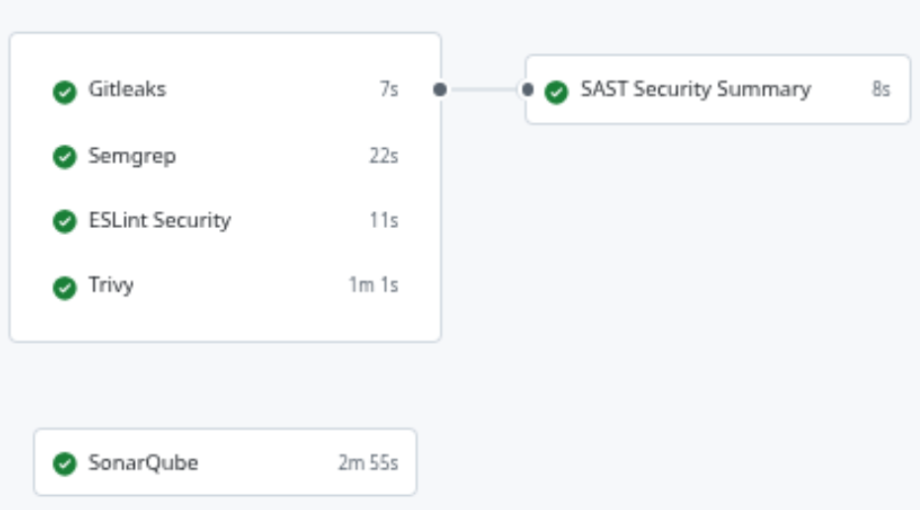
\includegraphics[width=0.90\linewidth]{workflow_pr.png}
  \caption{GitHub Actions PR workflow -- all jobs passed (Gitleaks 7s, Semgrep 22s, ESLint 11s, Trivy 1m1s, SonarQube 2m55s)}
\end{figure}

\begin{figure}[H]
  \centering
  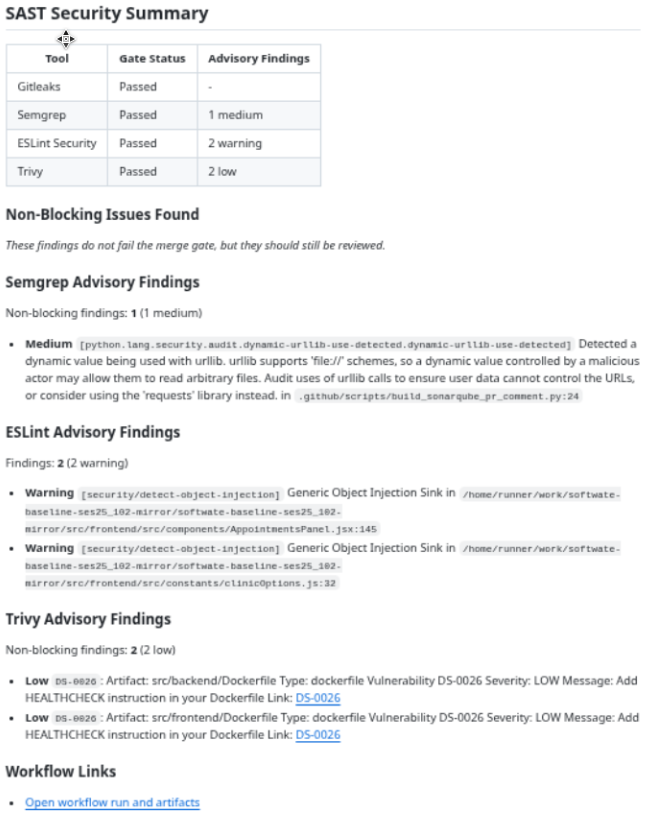
\includegraphics[width=0.85\linewidth]{sast_tools.png}
  \caption{SAST Security Summary PR comment -- advisory findings per tool}
\end{figure}

\begin{figure}[H]
  \centering
  \begin{minipage}[t]{0.48\linewidth}
    \centering
    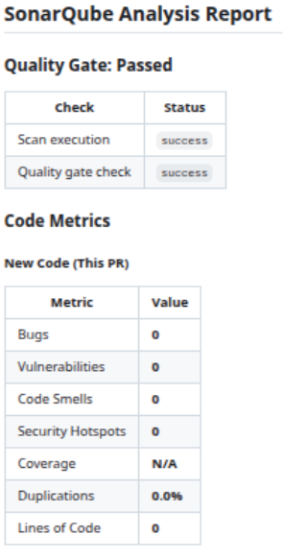
\includegraphics[width=\linewidth]{sq1.png}
    \caption{SonarQube Analysis Report -- Quality Gate: Passed (new code metrics)}
  \end{minipage}\hfill
  \begin{minipage}[t]{0.48\linewidth}
    \centering
    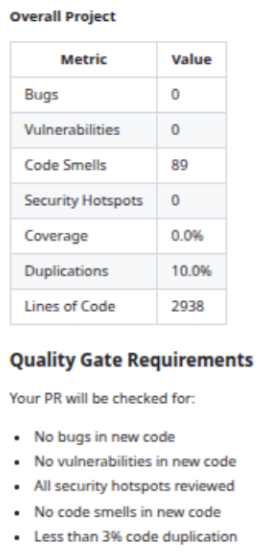
\includegraphics[width=\linewidth]{sq2.png}
    \caption{SonarQube -- Overall Project metrics (2938 LoC, 89 code smells)}
  \end{minipage}
\end{figure}

\begin{figure}[H]
  \centering
  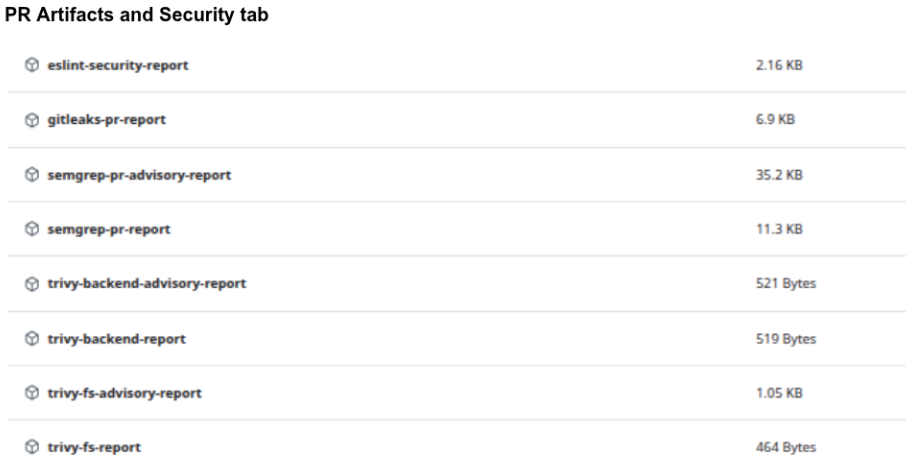
\includegraphics[width=0.90\linewidth]{sq_artifacts.png}
  \caption{PR artifacts -- reports uploaded by the SAST pipeline per tool}
\end{figure}

\subsection{Nightly Results}

\textbf{CodeQL:} No problems found. Scanned: GitHub Actions (3/3), Java (10/11), JavaScript (9/9).

\textbf{Semgrep:} Status Passed -- 0 findings across all severities.

\textbf{Trivy Image Scan:}

\begin{table}[H]
\centering
\caption{Trivy image scan -- nightly}
\begin{tabularx}{\linewidth}{l l X}
\toprule
\textbf{Image} & \textbf{Status} & \textbf{Notable CVEs} \\
\midrule
Backend  & Failed & CVE-2025-24734 (HIGH) -- \texttt{tomcat-embed-core} 11.0.15, fixed in 11.0.18 \\
Frontend & Failed & libcrypto3 CVE-2025-15467 (CRITICAL), libssl3, libc6, and multiple npm packages with HIGH CVEs \\
\bottomrule
\end{tabularx}
\end{table}

The nightly level confirms the value of deeper scheduled analysis: even though pre-commit and PR stages passed, Trivy image scanning detected significant vulnerabilities in the container image layers that were not visible at static code level.

\begin{figure}[H]
  \centering
  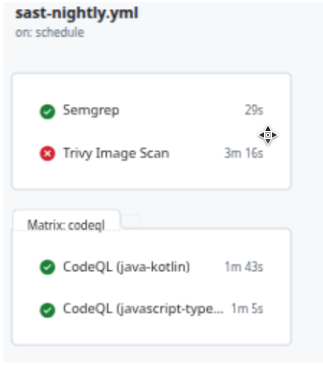
\includegraphics[width=0.70\linewidth]{nightly.png}
  \caption{Nightly SAST workflow -- Semgrep (29s), Trivy Image Scan (3m16s), CodeQL Java-Kotlin (1m43s), CodeQL JavaScript (1m5s)}
\end{figure}

\begin{figure}[H]
  \centering
  \begin{minipage}[t]{0.45\linewidth}
    \centering
    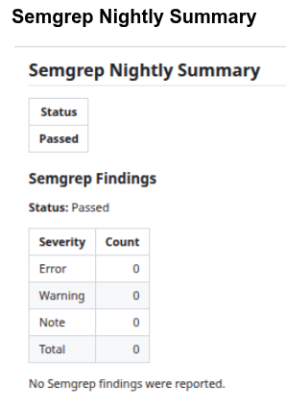
\includegraphics[width=\linewidth]{semgrep.png}
    \caption{Semgrep Nightly Summary -- Status: Passed, 0 findings}
  \end{minipage}\hfill
  \begin{minipage}[t]{0.52\linewidth}
    \centering
    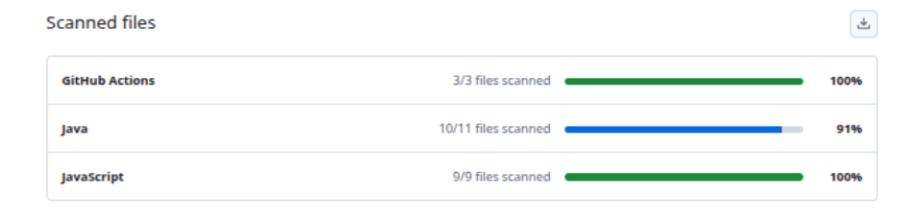
\includegraphics[width=\linewidth]{code_ql.png}
    \caption{CodeQL scanned files -- GitHub Actions 100\%, Java 91\%, JavaScript 100\%}
  \end{minipage}
\end{figure}

\begin{figure}[H]
  \centering
  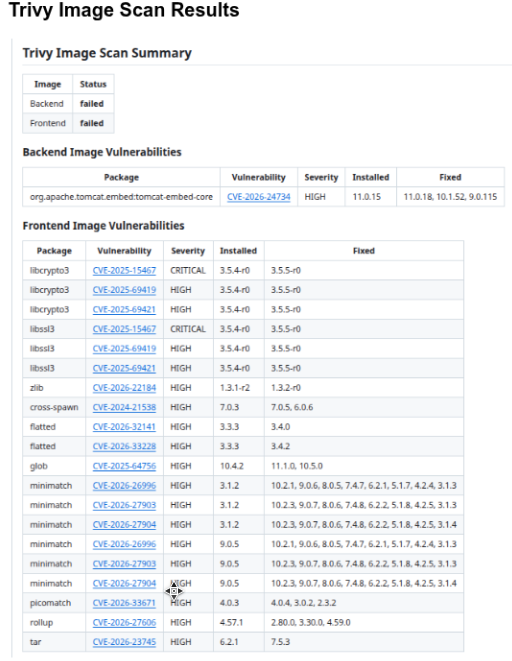
\includegraphics[width=0.80\linewidth]{trivy.png}
  \caption{Trivy Image Scan Results -- Backend (HIGH: tomcat-embed-core CVE-2025-24734) and Frontend (CRITICAL: libcrypto3 CVE-2025-15467 and multiple HIGH CVEs)}
\end{figure}

\begin{figure}[H]
  \centering
  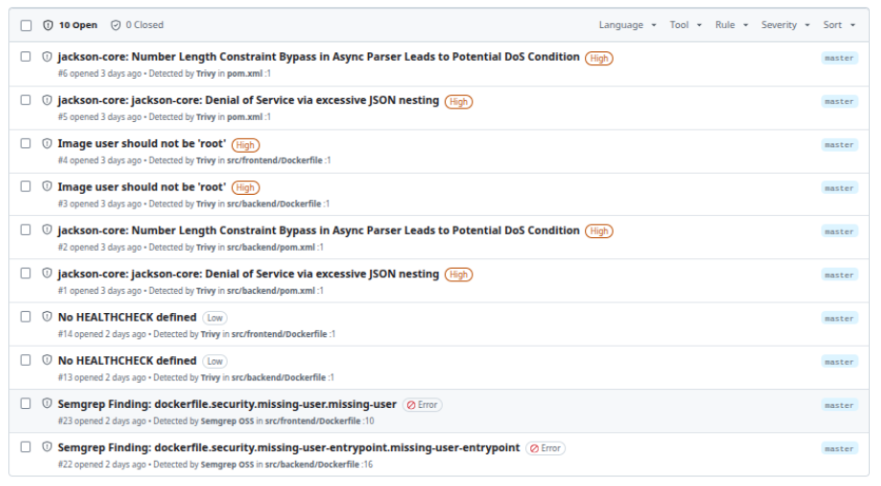
\includegraphics[width=\linewidth]{sq4.png}
  \caption{GitHub Security tab -- open alerts detected by Trivy (HIGH, pom.xml and Dockerfiles) and Semgrep (errors)}
\end{figure}

% ══════════════════════════════════════════════════════════════════════════════
\chapter{Dynamic Application Security Testing (DAST)}
% ══════════════════════════════════════════════════════════════════════════════

\section{Overview}

Dynamic Application Security Testing (DAST) assesses the running application from the outside, through its exposed web interface and HTTP endpoints, without relying on access to source code. Its purpose is to identify runtime security issues such as missing security headers, weak transport settings, unsafe default behaviour, exposed administrative functionality, and other vulnerabilities that become visible only when the application is deployed and reachable.

For this project, DAST is organised as a two-level process: a pull request level for merge-time validation, and a nightly level for recurring coverage against a stable target branch.

% ─────────────────────────────────────────────────────────────────────────────
\section{Objectives}
% ─────────────────────────────────────────────────────────────────────────────

\begin{itemize}
  \item Detect runtime security weaknesses in the deployed application.
  \item Validate the behaviour of the frontend and backend when exposed through HTTP.
  \item Provide merge-time and recurring feedback through GitHub Actions.
  \item Support the wider application security assessment together with SAST and manual pentesting.
\end{itemize}

% ─────────────────────────────────────────────────────────────────────────────
\section{Scope}
% ─────────────────────────────────────────────────────────────────────────────

The dynamic analysis scope covers the running ClinicWave application deployed in an ephemeral Docker-based environment. This includes the React/Vite frontend, the Spring Boot backend, the PostgreSQL database, the HTTP routes exposed by the frontend, and the backend endpoints reachable through the application during scanning.

% ─────────────────────────────────────────────────────────────────────────────
\section{Two-Level DAST Strategy}
% ─────────────────────────────────────────────────────────────────────────────

\subsection{Pull Request Level}

Runs through \texttt{dast-pr.yml}. The workflow builds the frontend and backend from the PR branch, starts a temporary PostgreSQL container, brings the full application up inside a dedicated Docker network, waits for both services to become reachable, and then runs an OWASP ZAP Baseline scan against the frontend entry point.

The PR gate is configured to fail when the ZAP report contains High severity findings. The workflow also generates both HTML and JSON ZAP reports, uploads them as workflow artefacts, evaluates the JSON output, and posts a DAST summary comment back to the pull request.

\subsection{Nightly Level}

Runs through \texttt{dast-nightly.yml}. This workflow checks out the software repository, builds and launches the full stack inside an isolated Docker environment, and scans with OWASP ZAP Baseline against the running frontend. It produces HTML and JSON ZAP reports, uploads them as artefacts, and writes a summarised view of alert counts and alert types into the workflow summary.

\subsection{Why the Two Levels Matter}

The pull request level provides merge-time validation and direct reviewer visibility. The nightly level provides recurring security monitoring against a stable target branch. This separation is useful because runtime scanning is slower and more environment-dependent than static analysis, so it benefits from having one layer optimised for gating and another for ongoing observation.

% ─────────────────────────────────────────────────────────────────────────────
\section{Runtime Environment and Tooling}
% ─────────────────────────────────────────────────────────────────────────────

Both workflows use \textbf{OWASP ZAP Baseline}. The application is launched inside Docker with a temporary PostgreSQL container, a backend container exposing the Spring Boot API, and a frontend container exposing the React/Vite application. The scanner targets the running frontend entry point.

% ─────────────────────────────────────────────────────────────────────────────
\section{Strengths and Limitations}
% ─────────────────────────────────────────────────────────────────────────────

\textbf{Strengths:} DAST validates the application in a running state, identifying issues only visible after deployment (missing headers, weak runtime defaults, exposed routes). GitHub Actions artefacts and PR comments make results easy to review and document.

\textbf{Limitations:} DAST depends on the application starting correctly in the test environment. A ZAP Baseline scan is more effective at identifying broad web security issues than deep business-logic flaws. Results quality depends on how much of the application surface the scanner can reach.

% ─────────────────────────────────────────────────────────────────────────────
\section{Results}
% ─────────────────────────────────────────────────────────────────────────────

\subsection{Pull Request Results}

The DAST workflow completed successfully. The gate passed because no \textbf{High} severity ZAP findings were detected.

\begin{figure}[H]
  \centering
  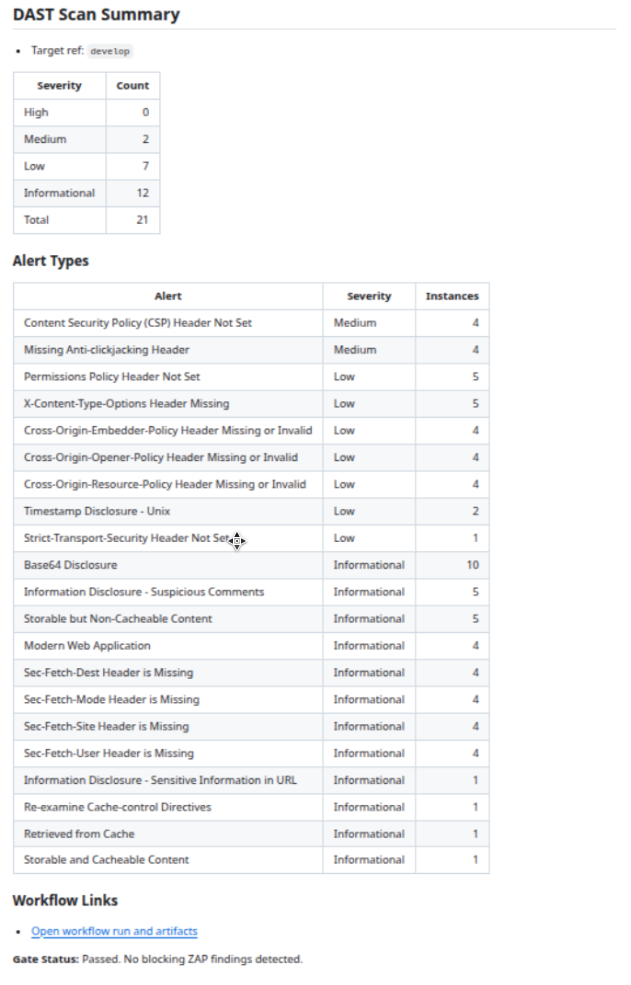
\includegraphics[width=0.72\linewidth]{DAST.png}
  \caption{DAST PR scan summary comment -- no High findings; gate status: Passed}
\end{figure}

\begin{table}[H]
\centering
\caption{DAST Scan Summary -- PR level}
\begin{tabular}{ll}
\toprule
\textbf{Severity} & \textbf{Count} \\
\midrule
High          & 0 \\
Medium        & 2 \\
Low           & 7 \\
Informational & 12 \\
\midrule
Total         & 21 \\
\bottomrule
\end{tabular}
\end{table}

\begin{table}[H]
\centering
\caption{DAST alert types -- PR level}
\begin{tabularx}{\linewidth}{X l r}
\toprule
\textbf{Alert} & \textbf{Severity} & \textbf{Instances} \\
\midrule
Content Security Policy (CSP) Header Not Set & Medium & 8 \\
Missing Anti-clickjacking Header             & Medium & 4 \\
Permissions Policy Header Not Set            & Low    & 5 \\
X-Content-Type-Options Header Missing        & Low    & 5 \\
Cross-Origin-Embedder-Policy Header Missing  & Low    & 4 \\
Cross-Origin-Opener-Policy Header Missing    & Low    & 4 \\
Cross-Origin-Resource-Policy Header Missing  & Low    & 4 \\
Timestamp Disclosure -- Unix                 & Low    & 2 \\
Strict-Transport-Security Header Not Set     & Low    & 1 \\
Base64 Disclosure                            & Informational & 10 \\
Information Disclosure -- Suspicious Comments & Informational & 5 \\
Storable but Non-Cacheable Content           & Informational & 5 \\
Modern Web Application                       & Informational & 8 \\
\bottomrule
\end{tabularx}
\end{table}

\begin{figure}[H]
  \centering
  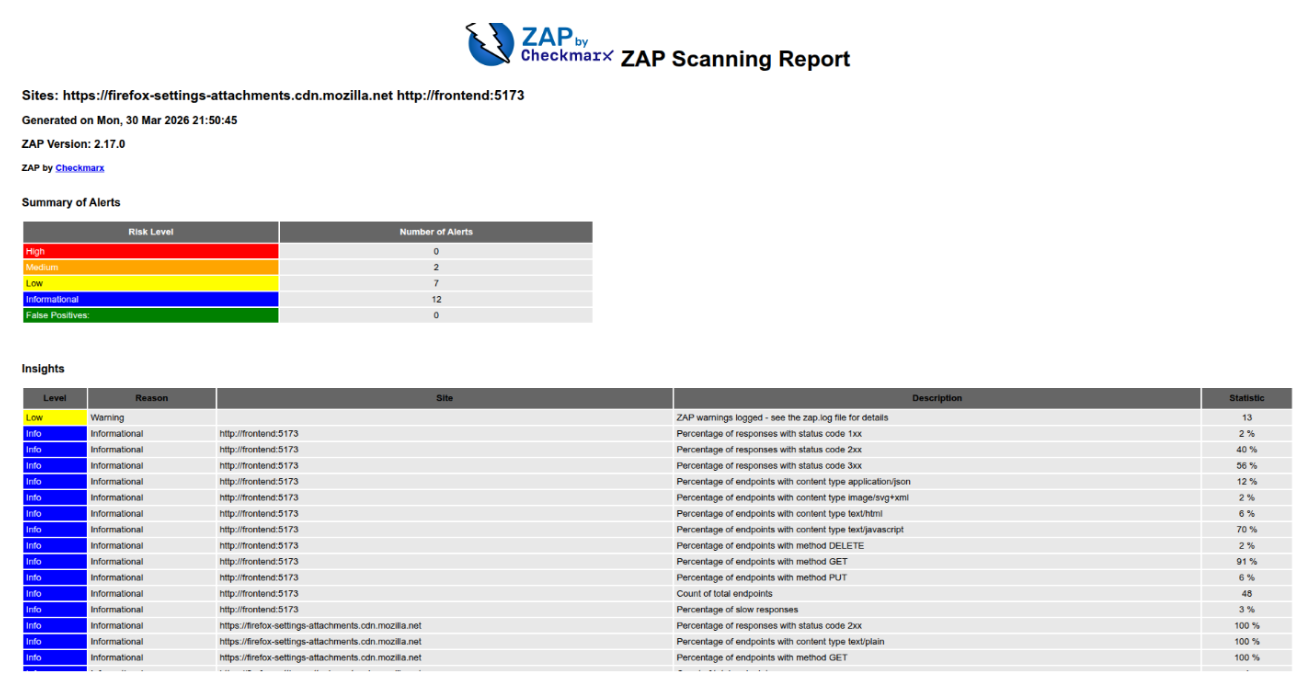
\includegraphics[width=\linewidth]{Zap.png}
  \caption{ZAP Scanning Report (HTML) -- PR run, generated Mon 30 Mar 2026}
\end{figure}

\begin{figure}[H]
  \centering
  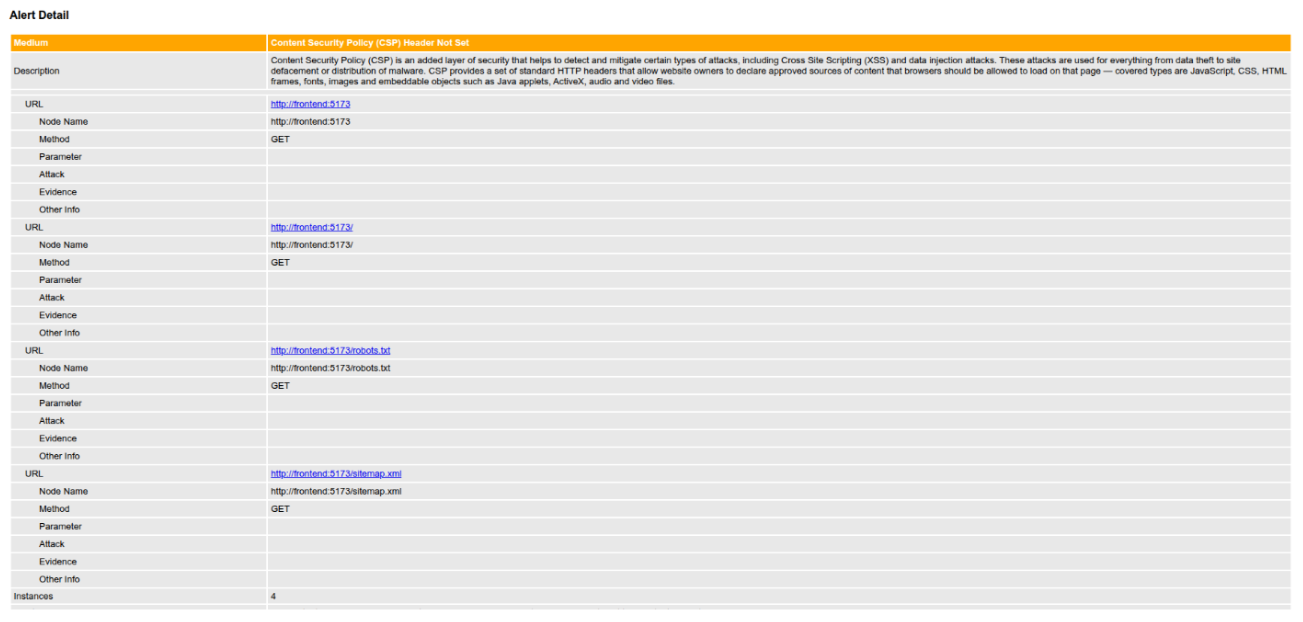
\includegraphics[width=\linewidth]{alert_detail_zap.png}
  \caption{ZAP Alert Detail -- Content Security Policy (CSP) Header Not Set (Medium, 4 instances)}
\end{figure}

\begin{figure}[H]
  \centering
  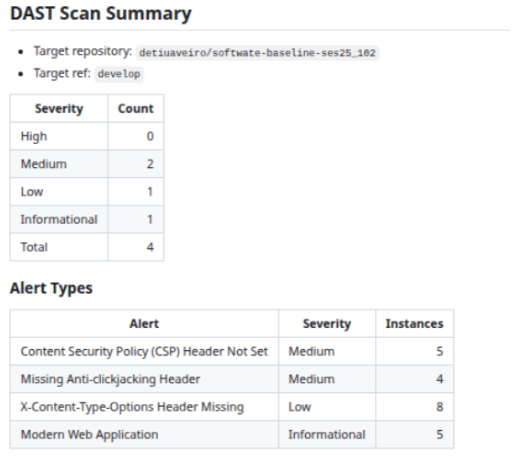
\includegraphics[width=0.72\linewidth]{DAST_ZAP_2.png}
  \caption{DAST alert types summary -- latest PR scan (4 alert types, High: 0)}
\end{figure}

\subsection{Nightly Results}

The nightly DAST workflow built and launched the full stack inside Docker and ran OWASP ZAP Baseline against the running frontend.

\begin{table}[H]
\centering
\caption{DAST Scan Summary -- Nightly level}
\begin{tabular}{ll}
\toprule
\textbf{Severity} & \textbf{Count} \\
\midrule
High          & 0 \\
Medium        & 2 \\
Low           & 1 \\
Informational & 1 \\
\midrule
Total         & 4 \\
\bottomrule
\end{tabular}
\end{table}

\begin{table}[H]
\centering
\caption{DAST alert types -- Nightly level}
\begin{tabularx}{\linewidth}{X l r}
\toprule
\textbf{Alert} & \textbf{Severity} & \textbf{Instances} \\
\midrule
Content Security Policy (CSP) Header Not Set & Medium & 5 \\
Missing Anti-clickjacking Header             & Medium & 4 \\
X-Content-Type-Options Header Missing        & Low    & 6 \\
Modern Web Application                       & Informational & 5 \\
\bottomrule
\end{tabularx}
\end{table}

The nightly results confirm the same top findings as the PR scan. No High severity findings were detected in either run. The nightly level provides a recurring view of the runtime security posture of the project even when no pull request is being reviewed.

\begin{figure}[H]
  \centering
  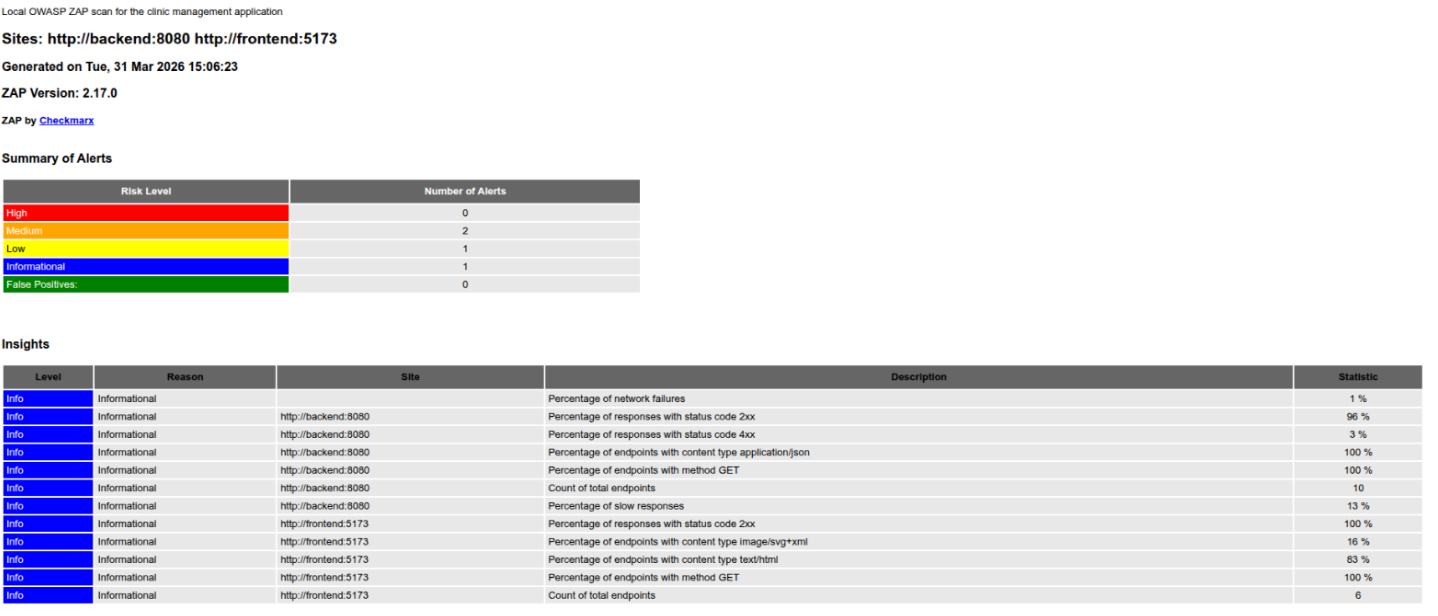
\includegraphics[width=\linewidth]{nightly_zap_2.png}
  \caption{Nightly ZAP Scanning Report (HTML) -- Local OWASP ZAP scan, generated Tue 31 Mar 2026}
\end{figure}

\begin{figure}[H]
  \centering
  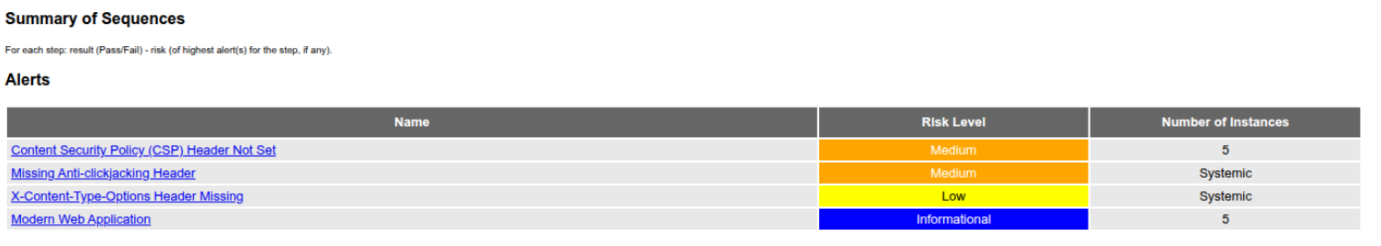
\includegraphics[width=\linewidth]{nightly_zap.png}
  \caption{Nightly ZAP Summary of Sequences -- alert breakdown: Medium (CSP, Anti-clickjacking), Low (X-Content-Type), Informational (Modern Web App)}
\end{figure}

% ══════════════════════════════════════════════════════════════════════════════
\chapter{Part 2 -- Security Fixes \& Architecture}
% ══════════════════════════════════════════════════════════════════════════════

Building on the Part 1 assessment, Part 2 fixes the vulnerabilities identified and introduces
a structured security architecture. The baseline had no authentication, no authorisation, no
input validation, and no perimeter controls. This chapter documents the changes made by
Tomás Brás (N\textsuperscript{o} 112665) -- API hardening, role-based access control,
authentication flow documentation, Zero Trust Architecture framing, and abuse story
regression -- and references the Keycloak/OIDC integration carried out by Afonso Ferreira.

% ─────────────────────────────────────────────────────────────────────────────
\section{Authentication \& Identity Management}
% ─────────────────────────────────────────────────────────────────────────────

\subsection{Overview}

The baseline had no authentication layer. The new architecture introduces Keycloak 26.2.5
as the external Identity Provider (IdP), using OpenID Connect (OIDC) with the
Authorization Code + PKCE (S256) flow. The backend validates every incoming request against
a signed JWT (RS256) fetched from the Keycloak JWKS endpoint.

\subsection{Token-Based Authentication}

\begin{itemize}
  \item \textbf{Access tokens} -- short-lived JWTs signed with RS256; validated on every request.
  \item \textbf{Refresh tokens} -- long-lived; used by \texttt{keycloak-js} to silently renew access tokens
        before expiry. Keycloak handles rotation and reuse detection server-side.
  \item \textbf{CSRF} -- the API is stateless and uses Bearer tokens only (no cookies), so CSRF
        is structurally inapplicable and is explicitly disabled in \texttt{SecurityConfig}.
\end{itemize}

\subsection{Authentication Flows}

\subsubsection{Login Flow}

\begin{enumerate}
  \item User opens the app. \texttt{keycloak.init(\{onLoad: 'login-required', pkceMethod: 'S256'\})} is
        called before any React component renders.
  \item If no valid session exists, the browser is redirected to the Keycloak login page.
  \item The user authenticates (username + password). Keycloak verifies the credential and
        issues an authorisation code.
  \item PKCE: the frontend sends the stored \texttt{code\_verifier}; Keycloak verifies the
        \texttt{code\_challenge} (SHA-256) and returns an access token + refresh token.
  \item Tokens are stored in memory by \texttt{keycloak-js}. The frontend proceeds to render.
  \item Each API call in \texttt{httpConsumer.js} adds \texttt{Authorization: Bearer <token>} to the request.
  \item The Spring Boot backend receives the token, fetches the JWKS from Keycloak lazily
        (\texttt{NimbusJwtDecoder}), validates the RS256 signature, checks the \texttt{iss} claim
        (\texttt{JwtValidators.createDefaultWithIssuer}), and extracts roles via \texttt{JwtRoleConverter}.
\end{enumerate}

\subsubsection{Logout Flow}

\begin{enumerate}
  \item The user clicks the \textbf{Logout} button in the top navigation bar.
  \item The frontend calls \path{keycloak.logout()} with a \texttt{redirectUri} set to the current application origin.
  \item Keycloak invalidates the session server-side (back-channel logout), clears the SSO
        cookie, and redirects the browser back to the application origin.
  \item The app re-enters \texttt{keycloak.init()} and redirects to the Keycloak login page.
\end{enumerate}

\subsubsection{Token Refresh Flow}

\begin{enumerate}
  \item Before every API request, \path{httpConsumer.js} calls
        \texttt{await keycloak.\allowbreak{}updateToken(30)}.
  \item If the access token expires within 30 seconds, \texttt{keycloak-js} sends the refresh
        token to Keycloak's token endpoint and obtains a new access token silently.
  \item If the refresh token is also expired, \texttt{keycloak.login()} is called, redirecting
        the user back to the login page with no data loss.
\end{enumerate}

\subsubsection{Token Revocation}

Keycloak handles revocation server-side. When a user logs out, the session (and all tokens
associated with it) is invalidated. If an administrator disables or deletes a user in
Keycloak, existing tokens will fail issuer/audience validation on the next backend call
(or on the next refresh attempt, whichever comes first).

\subsection{Roles and Realm Configuration}

Three roles are defined in the Keycloak realm (\texttt{clinic}):

\begin{table}[H]
\centering
\caption{Keycloak roles and default permissions}
\begin{tabularx}{\linewidth}{l X X}
\toprule
\textbf{Role}       & \textbf{Patients}              & \textbf{Appointments} \\
\midrule
ADMIN               & READ, CREATE, UPDATE, DELETE   & READ, CREATE, UPDATE, DELETE \\
DOCTOR              & READ, UPDATE                   & READ, UPDATE \\
RECEPTIONIST        & READ, CREATE                   & READ, CREATE, UPDATE, DELETE \\
\bottomrule
\end{tabularx}
\end{table}

Users (\texttt{admin}, \texttt{doctor}, \texttt{receptionist}) are assigned to their
corresponding realm roles in the Keycloak admin console. The \texttt{clinic-frontend} client
uses the Authorization Code + PKCE flow; \texttt{directAccessGrantsEnabled} is enabled to
allow \texttt{curl}-based testing in development.

% ─────────────────────────────────────────────────────────────────────────────
\section{Explicit Authorization Layer (RBAC)}
% ─────────────────────────────────────────────────────────────────────────────

\subsection{Design}

Role-Based Access Control is implemented at two layers:

\begin{description}
  \item[\textbf{Route-level}] \texttt{SecurityConfig} requires authentication on all
    \texttt{/api/**} routes and uses \texttt{anyRequest().denyAll()} as the catch-all
    (deny-by-default). No unauthenticated request reaches a controller.
  \item[\textbf{Method-level}] Every controller method is annotated with
    \texttt{@PreAuthorize} referencing the \texttt{@perms} bean:
    \texttt{@perms.canAnyRole(authentication,\allowbreak{} '<resource>',\allowbreak{} '<action>')}.
    The bean checks the caller's granted authorities against the permissions matrix
    loaded from \texttt{application.yml}.
\end{description}

\subsection{Permissions as Data}

Roles and their allowed actions are expressed as a configuration file, not embedded in
controller logic. \texttt{application.yml} defines the full matrix:

\begin{table}[H]
\centering\small
\caption{Permissions matrix (\texttt{application.yml})}
\begin{tabular}{llll}
\toprule
\textbf{Role}  & \textbf{Resource}    & \textbf{Allowed actions} \\
\midrule
ADMIN          & patients             & READ, CREATE, UPDATE, DELETE \\
ADMIN          & appointments         & READ, CREATE, UPDATE, DELETE \\
DOCTOR         & patients             & READ, UPDATE \\
DOCTOR         & appointments         & READ, UPDATE \\
RECEPTIONIST   & patients             & READ, CREATE \\
RECEPTIONIST   & appointments         & READ, CREATE, UPDATE, DELETE \\
\bottomrule
\end{tabular}
\end{table}

The \texttt{PermissionsConfig} class is annotated with \texttt{@Component("perms")} and
\texttt{@ConfigurationProperties(prefix = "clinic")}. Its \texttt{canAnyRole} method
iterates over the caller's Spring Security granted authorities and checks each against
the map, returning \texttt{true} if any role grants the requested action.

\subsection{Object-Level Authorization (BOLA)}

Each service method returns \texttt{Optional.empty()} when a resource ID does not exist.
Controllers map this to HTTP 404. Because all endpoints require a valid JWT and
role-based permission, an authenticated caller with the correct role who requests a
non-existent resource receives 404 rather than 403, preventing ID enumeration by
response differentiation.

\subsection{Role-Based UI}

The frontend enforces the same permission matrix client-side using the \texttt{usePermissions}
hook (\texttt{src/auth/usePermissions.js}). The hook reads \texttt{realm\_access.roles} from
the decoded JWT token and returns a \texttt{can(resource, action)} function. Buttons that
the current user's role does not permit are not rendered:

\begin{itemize}
  \item \textbf{Admin}: sees all New / Edit / Delete buttons for both patients and appointments.
  \item \textbf{Doctor}: sees Edit on patients (READ + UPDATE); sees Edit on appointments only.
  \item \textbf{Receptionist}: sees New Patient and Edit (no Delete); sees all appointment actions.
\end{itemize}

This is a UX control only -- the backend enforces the same rules independently.

\subsection{Unit Tests}

\texttt{RbacTest.java} covers all role $\times$ action $\times$ resource combinations using
Spring Boot's \texttt{MockMvc} with the \texttt{jwt()} security post-processor from
\texttt{spring-security-test}. Tests verify:

\begin{itemize}
  \item Unauthenticated requests → HTTP 401.
  \item Authenticated requests with an insufficient role → HTTP 403.
  \item Authenticated requests with the correct role but a missing resource → HTTP 404.
\end{itemize}

21 tests in total; all pass without a running Keycloak instance because the JWKS decoder
is lazy and the \texttt{jwt()} post-processor bypasses token validation.

% ─────────────────────────────────────────────────────────────────────────────
\section{API Hardening -- OWASP API Top 10 (2023)}
% ─────────────────────────────────────────────────────────────────────────────

Each control below is traceable to an OWASP API Security item and to the corresponding
commit on the \texttt{develop} branch.

\begin{longtable}{S{0.9cm} S{2.1cm} S{4.8cm} S{5.8cm}}
\caption{OWASP API Top 10 coverage}\label{tab:owasp}\\
\toprule
\textbf{Item} & \textbf{Category} & \textbf{Vulnerability (baseline)} & \textbf{Control implemented} \\
\midrule
\endfirsthead
\multicolumn{4}{l}{\small\textit{(continued)}}\\
\toprule
\textbf{Item} & \textbf{Category} & \textbf{Vulnerability (baseline)} & \textbf{Control implemented} \\
\midrule
\endhead
\bottomrule
\endfoot

API1 & BOLA & No per-object ownership check; any caller can read or modify any record by ID. &
\texttt{@PreAuthorize} on every endpoint; service returns 404 for non-existent resources, preventing ID oracle. \\[6pt]

API3 & BOPLA & Controllers bound JPA entities directly; any JSON field was writable. &
\texttt{PatientRequestDTO} and \texttt{AppointmentRequestDTO} constrain the accepted surface. \texttt{@Valid} with Bean Validation (\texttt{@NotBlank}, \texttt{@NotNull}, \texttt{@Past}, \texttt{@Email}, \texttt{@Pattern}) rejects malformed input before the service layer. \\[6pt]

API4 & Resource Consumption & No rate limiting; no request-size limits; unbounded full-table scans possible. &
\texttt{RateLimitFilter} (token-bucket, 60\,req/min per IP) on all \texttt{/api/**} routes. Request-size limits set to 1\,MB via Tomcat (\texttt{max-http-form-post-size}) and Spring multipart (\texttt{max-request-size}, \texttt{max-file-size}). \\[6pt]

API5 & Function-Level Auth & All endpoints accessible to any unauthenticated caller; no deny-by-default. &
\texttt{SecurityConfig} uses \texttt{anyRequest().\allowbreak denyAll()} as the catch-all. All \texttt{/api/**} requires authentication. No route is reachable without a valid JWT. \\[6pt]

API8 & Security Misconfiguration & No security headers; no CSRF/frame protection; stack traces in error responses. &
\texttt{SecurityConfig} configures HSTS, \texttt{X-Frame-Options: DENY}, \texttt{X-Content-Type-Options}, and \texttt{Content-Security-Policy: default-src 'none'}. Form login and HTTP Basic are disabled. \\[6pt]

API9 & Improper Inventory & No API documentation or endpoint inventory. &
\texttt{springdoc-openapi} generates an OpenAPI\,3 spec at \texttt{/v3/api-docs}; Swagger UI at \texttt{/swagger-ui.html}. Both are \texttt{permitAll()}. All endpoints annotated with \texttt{@Operation} and \texttt{@Tag}. \\
\end{longtable}

% ─────────────────────────────────────────────────────────────────────────────
\section{Perimeter Defense}
% ─────────────────────────────────────────────────────────────────────────────

A reverse proxy with an embedded Web Application Firewall is placed in front of the
application, providing a perimeter enforcement layer that is independent of the backend
business logic.

\subsection{Nginx + ModSecurity CRS}

The perimeter is implemented as a dedicated Docker container built on the
\texttt{owasp/modsecurity-crs:nginx-alpine} base image. It sits between the external
network and the frontend/backend containers.

\begin{table}[H]
\centering
\caption{Perimeter defense configuration summary}
\begin{tabularx}{\linewidth}{l X}
\toprule
\textbf{Property} & \textbf{Value} \\
\midrule
Engine              & Nginx + ModSecurity v3 \\
Ruleset             & OWASP Core Rule Set (CRS) -- blocking mode (\texttt{SecRuleEngine On}) \\
Paranoia Level      & 1 (balanced: broad coverage, low false-positive rate) \\
Inbound threshold   & 5 (anomaly score to block a request) \\
Outbound threshold  & 4 \\
TLS termination     & Self-signed certificate via \texttt{mkcert}; HTTPS on port 443 \\
Request body limit  & 1\,MB (\texttt{SecRequestBodyLimit 1048576}); excess is rejected \\
IP rate limiting    & Nginx \texttt{limit\_req\_zone} -- 30 req/s burst, 10 req/s sustained per IP \\
Audit logging       & \texttt{SecAuditEngine RelevantOnly} -- logs 4xx/5xx events \\
\bottomrule
\end{tabularx}
\end{table}

\subsection{CRS Tuning and False Positives}

Four false positive exclusions were added and are documented in
\path{waf/crs-setup.d/02-clinic-rule-exclusions.conf}:

\begin{table}[H]
\centering
\caption{CRS rule exclusions applied}
\begin{tabularx}{\linewidth}{S{1.5cm} S{2.8cm} X}
\toprule
\textbf{Rule} & \textbf{Trigger} & \textbf{Reason} \\
\midrule
920420 & Content-Type check & Spring Boot appends \texttt{; charset=UTF-8} to \texttt{application/json} in error responses; CRS requires an exact match without the charset parameter. \\
942100 & SQL injection (libinjection) & \texttt{patientName}, \texttt{specialty}, and \texttt{status} query parameters accept free-text (e.g.\ \emph{O'Brien}). The application uses JPA parameterised queries -- no raw SQL is executed. \\
942440 & SQL comment sequence & Specialty values such as \emph{Cardio--thoracic} contain a double-dash sequence that CRS flags as a SQL comment marker. \\
920230 & Multiple URL encoding & ISO\,8601 datetime strings submitted as JSON body can trigger double-encoding detection in some HTTP clients. \\
\bottomrule
\end{tabularx}
\end{table}

No legitimate requests are blocked after these exclusions. All four exclusions are scoped to
specific URI prefixes (\texttt{/api/patients}, \texttt{/api/appointments}) to minimise the
attack surface widened by each exclusion.

% ─────────────────────────────────────────────────────────────────────────────
\section{Zero Trust Architecture Framing}
% ─────────────────────────────────────────────────────────────────────────────

\subsection{NIST SP 800-207 Components}

The resulting architecture is framed below using the Zero Trust terminology from NIST SP 800-207.

\begin{table}[H]
\centering
\caption{NIST SP 800-207 ZTA component mapping}
\begin{tabularx}{\linewidth}{l X}
\toprule
\textbf{ZTA Component} & \textbf{Implementation} \\
\midrule
\textbf{Subject} &
  Clinic staff authenticated via Keycloak: users \texttt{admin}, \texttt{doctor},
  \texttt{receptionist} with assigned realm roles. Identity is asserted per-request
  via a signed JWT. \\[6pt]

\textbf{Policy Enforcement Point (PEP)} &
  Three layers: (1) Nginx + ModSecurity CRS -- perimeter WAF that filters and rate-limits
  all traffic before it reaches the application; (2) \texttt{SecurityFilterChain} -- enforces
  JWT presence on every \texttt{/api/**} request; (3) Spring \texttt{@PreAuthorize} annotations
  on each controller method -- enforce the role $\times$ resource $\times$ action permission. \\[6pt]

\textbf{Policy Decision Point (PDP)} &
  \texttt{PermissionsConfig} (\texttt{@Component("perms")}) evaluates the caller's
  granted authorities against the permissions matrix loaded from \texttt{application.yml}.
  The decision (allow / deny) is returned as a boolean to the PEP. \\[6pt]

\textbf{Policy Administrator (PA)} &
  Keycloak 26.2.5 -- manages user identities, realm roles, and client configuration.
  Issues signed JWTs; provides the JWKS endpoint for backend token validation.
  Administrators manage access through the Keycloak Admin Console. \\[6pt]

\textbf{Trust Algorithm} &
  Never-trust, always-verify: every request must carry a valid RS256 JWT. The
  backend re-validates the signature and \texttt{iss} claim on every call.
  No session state is maintained in the application -- the JWT is the sole credential. \\
\bottomrule
\end{tabularx}
\end{table}

\subsection{NIST SP 800-207 \S2.1 -- Seven Tenets Mapping}

\begin{longtable}{S{0.4cm} S{4.2cm} S{2.2cm} S{7.0cm}}
\caption{Zero Trust tenet compliance status}\label{tab:zta-tenets}\\
\toprule
\textbf{\#} & \textbf{Tenet} & \textbf{Status} & \textbf{Notes} \\
\midrule
\endfirsthead
\multicolumn{4}{l}{\small\textit{(continued)}}\\
\toprule
\textbf{\#} & \textbf{Tenet} & \textbf{Status} & \textbf{Notes} \\
\midrule
\endhead
\bottomrule
\endfoot

1 & All data sources and computing services are considered resources. &
  \textbf{Partial} &
  Patient records and appointment data are treated as protected resources. Device or service identity is not yet managed (no mTLS, no device posture). \\[6pt]

2 & All communication is secured regardless of network location. &
  \textbf{Partial} &
  TLS is terminated at the Nginx WAF (self-signed certificate via \texttt{mkcert}; HTTPS on
  port 443). All API communication is bearer-token authenticated (JWT RS256). Inter-container
  communication (WAF $\to$ backend) is over the private Docker network without additional
  TLS; mTLS for service-to-service channels remains future work. \\[6pt]

3 & Access to individual enterprise resources is granted on a per-session basis. &
  \textbf{Met} &
  Short-lived JWTs are issued per Keycloak session. The frontend requests a new token before each call (\texttt{updateToken(30)}). No persistent session state is stored in the backend. \\[6pt]

4 & Access to resources is determined by dynamic policy. &
  \textbf{Met} &
  The permissions matrix in \texttt{application.yml} is evaluated dynamically at method-invocation time. Role assignment is controlled in Keycloak and reflected in the JWT \texttt{realm\_access.roles} claim without requiring a redeploy. \\[6pt]

5 & The enterprise monitors and measures the integrity and security posture of all owned and associated assets. &
  \textbf{Not met} &
  No asset monitoring, endpoint posture assessment, or SIEM integration exists. Flagged as \textbf{future work}. \\[6pt]

6 & All resource authentication and authorisation is dynamic and strictly enforced before access is allowed. &
  \textbf{Met} &
  Every \texttt{/api/**} request is authenticated. Every controller method checks the caller's role before the service layer is reached. Deny-by-default (\texttt{anyRequest().denyAll()}) ensures no route is reachable without a valid JWT and sufficient role. \\[6pt]

7 & The enterprise collects as much information as possible about the current state of assets, network infrastructure, and communications. &
  \textbf{Not met} &
  No structured audit log, access log, or security event stream is implemented. Actor identity is now available in the JWT (addresses R-02), but CRUD operations are not persisted to an audit trail. Flagged as \textbf{future work}. \\
\end{longtable}

% ─────────────────────────────────────────────────────────────────────────────
\section{Abuse Story Regression}
% ─────────────────────────────────────────────────────────────────────────────

Each abuse story from Part 1 is re-evaluated against the security controls now in place.
Classification follows the three categories defined in the project specification:
\textbf{prevented} (attack is no longer feasible), \textbf{detected} (attack is possible
but leaves a trace), or \textbf{residual risk} (risk remains and must be managed).

\begin{longtable}{S{1.0cm} S{3.8cm} S{2.4cm} S{6.5cm}}
\caption{Abuse story regression}\label{tab:regression}\\
\toprule
\textbf{ID} & \textbf{Title} & \textbf{Status} & \textbf{Justification} \\
\midrule
\endfirsthead
\multicolumn{4}{l}{\small\textit{(continued)}}\\
\toprule
\textbf{ID} & \textbf{Title} & \textbf{Status} & \textbf{Justification} \\
\midrule
\endhead
\bottomrule
\endfoot

AS-01 & Unauthorised Access to Patient Data &
  \textbf{\textcolor{sevlow}{Prevented}} &
  All \texttt{/api/**} endpoints now require a valid JWT. An unauthenticated request receives HTTP 401 before reaching any controller. The three attack paths (list dump, IDOR enumeration, appointment endpoint) are all blocked at the \texttt{SecurityFilterChain}. \\[8pt]

AS-02 & Link Patient Identity to Appointment History &
  \textbf{\textcolor{sevlow}{Prevented}} &
  Both \texttt{GET /api/patients} and \texttt{GET /api/appointments} require authentication and the READ role on the corresponding resource. An unauthenticated attacker cannot correlate patient and appointment records. \\[8pt]

AS-03 & Direct Patient Identification via IDOR &
  \textbf{\textcolor{sevlow}{Prevented}} &
  Authentication blocks unauthenticated enumeration. \texttt{RateLimitFilter} limits authenticated callers to 60 requests/min per IP, making brute-force enumeration impractical. Sequential IDs remain (future work: UUIDs). \\[8pt]

AS-04 & Infer Health Condition from Appointment Metadata &
  \textbf{\textcolor{sevlow}{Prevented}} &
  All appointment endpoints require a valid JWT and the READ role. An external attacker cannot query \texttt{GET /api/appointments?patientName=X} without authentication. \\[8pt]

AS-05 & Modify or Reassign Appointment Records &
  \textbf{\textcolor{sevlow}{Prevented}} &
  \texttt{PUT /api/appointments/\{id\}} requires UPDATE role. \texttt{AppointmentRequestDTO} constrains the writable fields (dateTime, specialty, status) and excludes the patient relationship, eliminating the silent rebind attack via nested objects. \\[8pt]

AS-06 & Destroy Patient Records via Cascade Deletion &
  \textbf{\textcolor{sevlow}{Prevented}} &
  \texttt{DELETE /api/patients/\{id\}} requires ADMIN role. Soft-delete is now implemented:
  \texttt{Patient} and \texttt{Appointment} carry a \texttt{deleted\_at} timestamp; deletion
  sets this field instead of issuing a SQL \texttt{DELETE}. \texttt{@SQLRestriction} on both
  entities filters soft-deleted records from all queries automatically. Cascade hard-deletion
  (\texttt{orphanRemoval}) has been removed. Data is never permanently destroyed by a single
  API call. \\[8pt]

AS-07 & Perform Undetectable Actions &
  \textbf{\textcolor{sevmedium}{Detected}} &
  A structured \texttt{audit\_logs} table now persists every CREATE, UPDATE, and DELETE
  operation with the JWT \texttt{sub} claim (actor), resource type, resource ID, and
  timestamp. The log is written synchronously within the same request. ADMIN users can
  query the full trail via \texttt{GET /api/audit-logs}. Post-incident investigation is
  now possible for all authenticated CRUD operations. \\[8pt]

AS-08 & Overload the API with Repeated Requests &
  \textbf{\textcolor{sevlow}{Prevented}} &
  Two independent rate-limiting layers are in place: (1) Nginx \texttt{limit\_req\_zone}
  enforces 30 req/s burst / 10 req/s sustained per IP at the perimeter; (2) Spring
  \texttt{RateLimitFilter} enforces 60 req/min per IP inside the application. ModSecurity CRS
  request-body limits (1\,MB) further constrain large-payload abuse. A highly distributed
  multi-IP attack remains a theoretical residual risk but is significantly harder with dual
  perimeter + application throttling. \\
\end{longtable}

\subsection{Regression Evidence}

The following figures present the regression diagrams produced for each abuse story, showing the original attack path, what changed in Part 2, and the resulting status.

\begin{figure}[H]
  \centering
  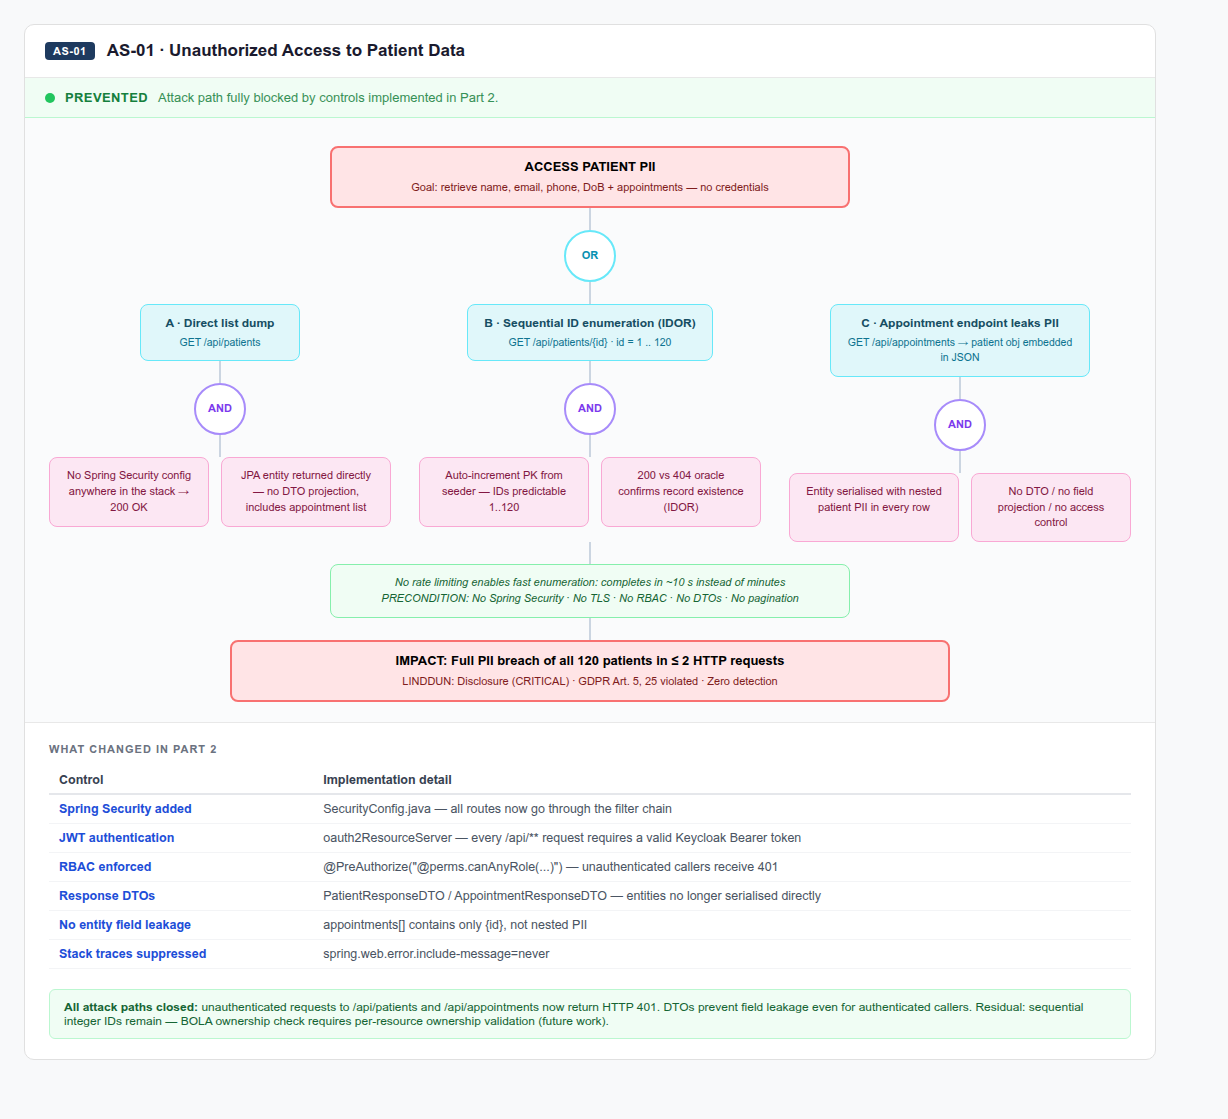
\includegraphics[width=\linewidth]{01_regression.png}
  \caption{AS-01 -- Unauthorised Access to Patient Data: \textbf{Prevented}}
\end{figure}

\begin{figure}[H]
  \centering
  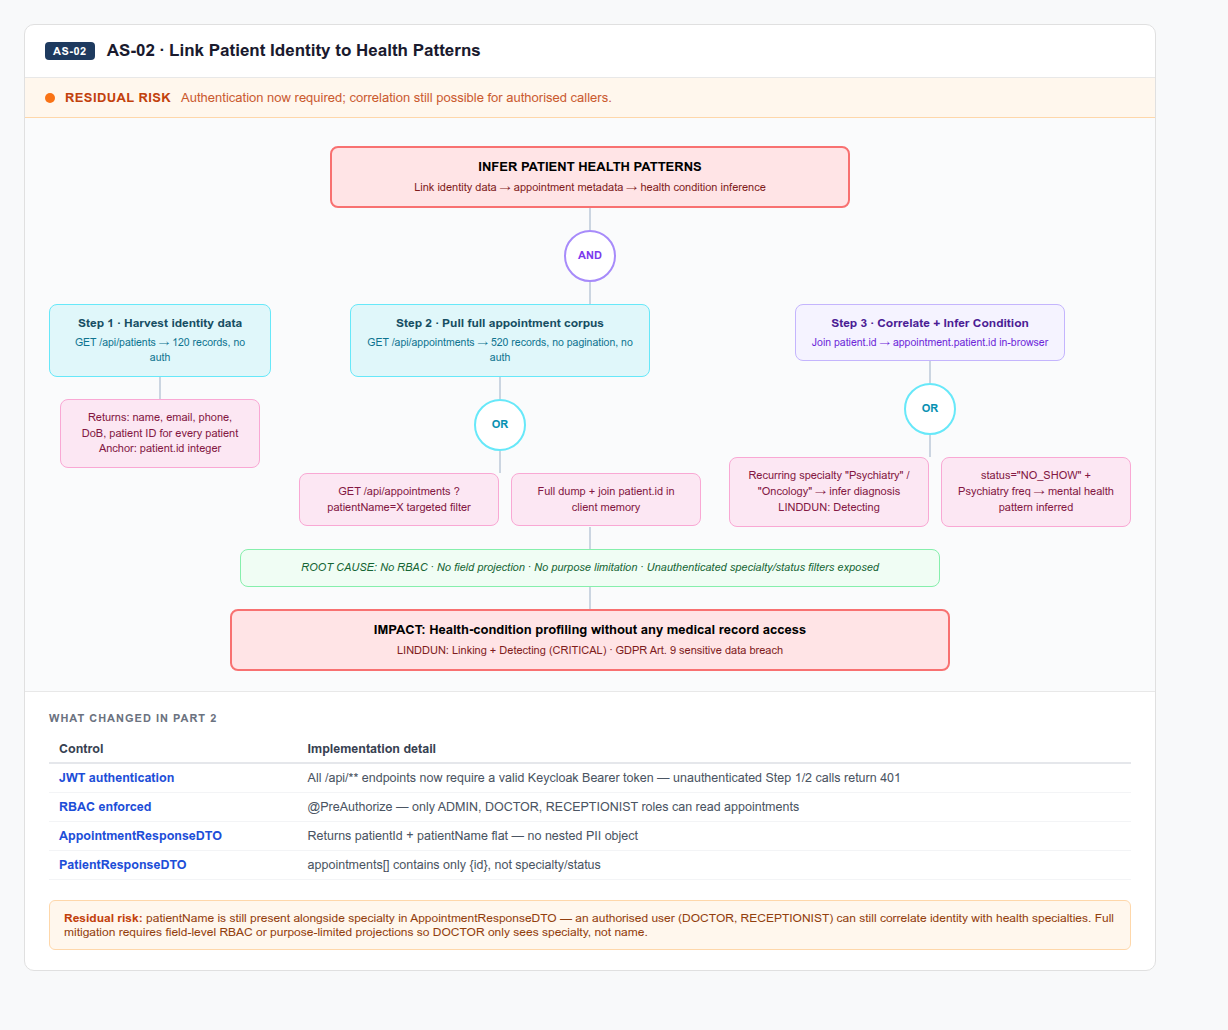
\includegraphics[width=\linewidth]{02_regression.png}
  \caption{AS-02 -- Link Patient Identity to Appointment History: \textbf{Prevented}}
\end{figure}

\begin{figure}[H]
  \centering
  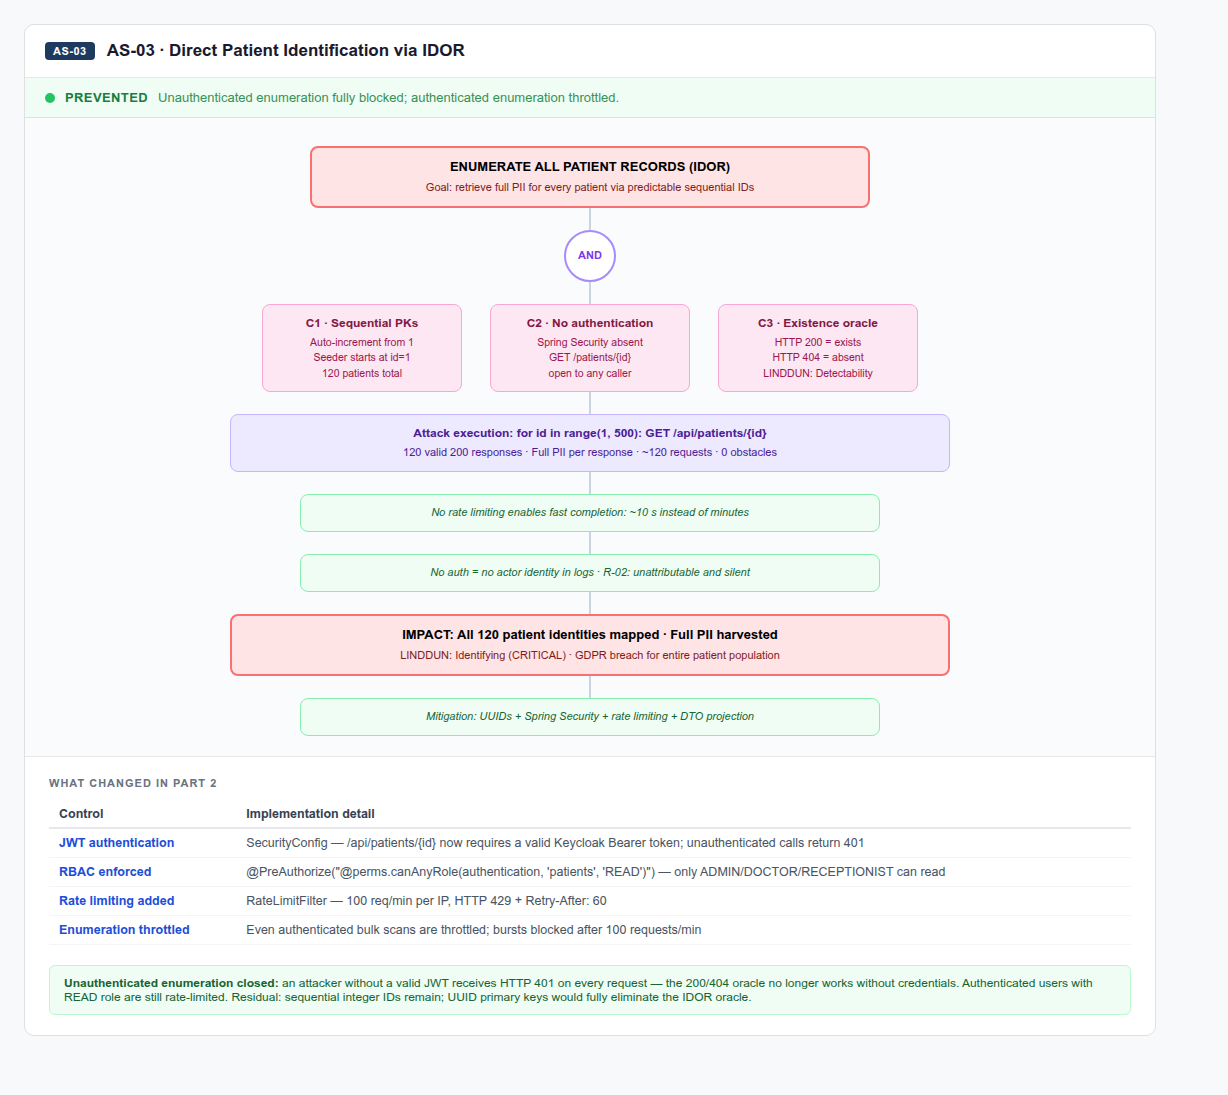
\includegraphics[width=\linewidth]{03_regression.png}
  \caption{AS-03 -- Direct Patient Identification via IDOR: \textbf{Prevented}}
\end{figure}

\begin{figure}[H]
  \centering
  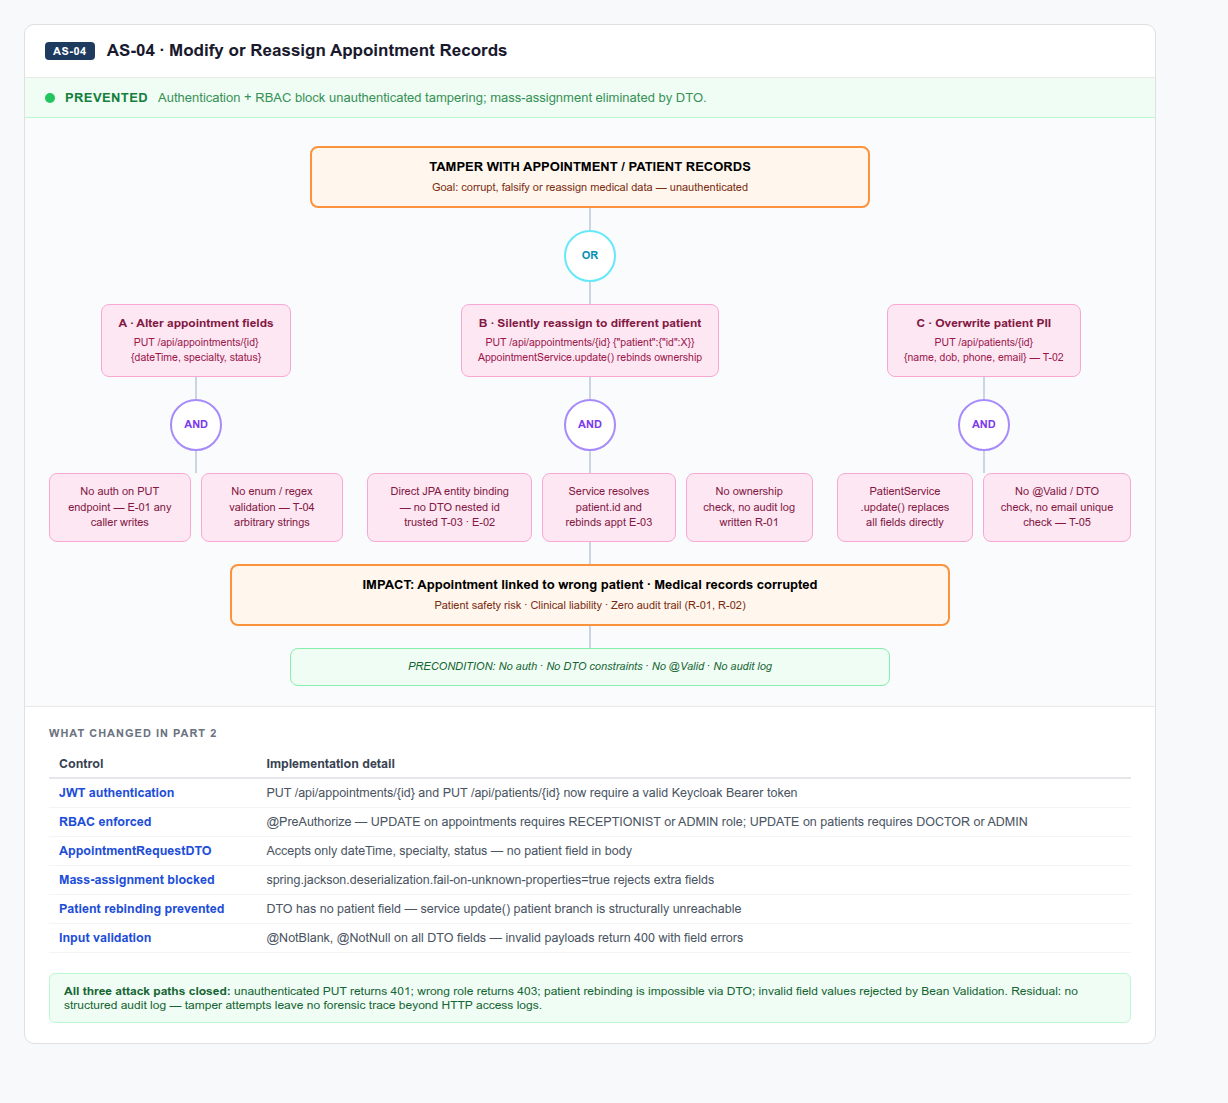
\includegraphics[width=\linewidth]{04_regression.png}
  \caption{AS-04 -- Infer Health Condition from Appointment Metadata: \textbf{Prevented}}
\end{figure}

\begin{figure}[H]
  \centering
  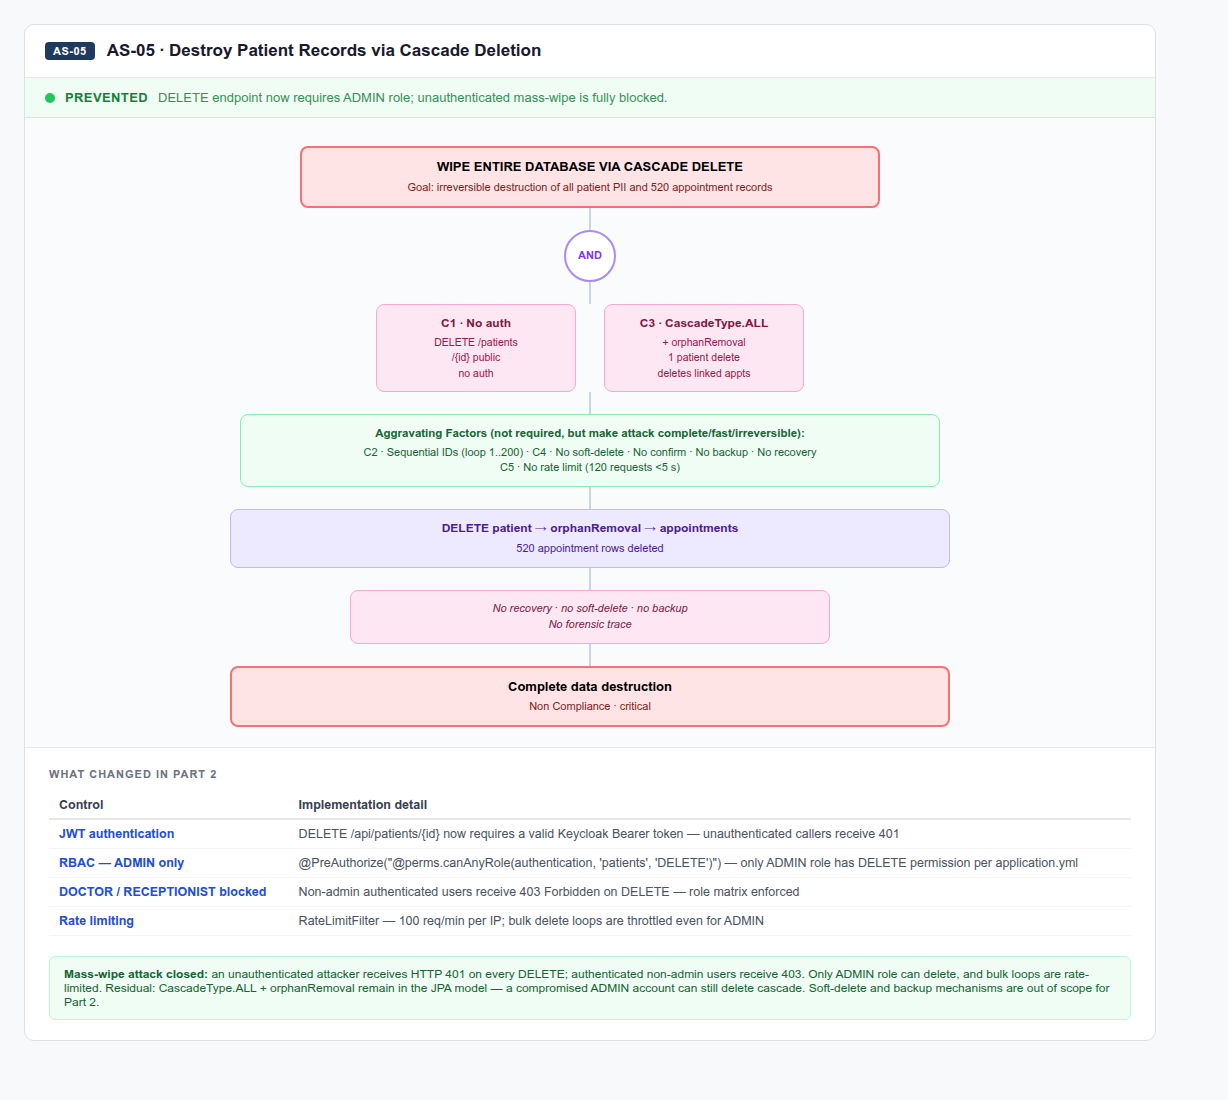
\includegraphics[width=\linewidth]{05_regression.png}
  \caption{AS-05 -- Modify or Reassign Appointment Records: \textbf{Prevented}}
\end{figure}

\begin{figure}[H]
  \centering
  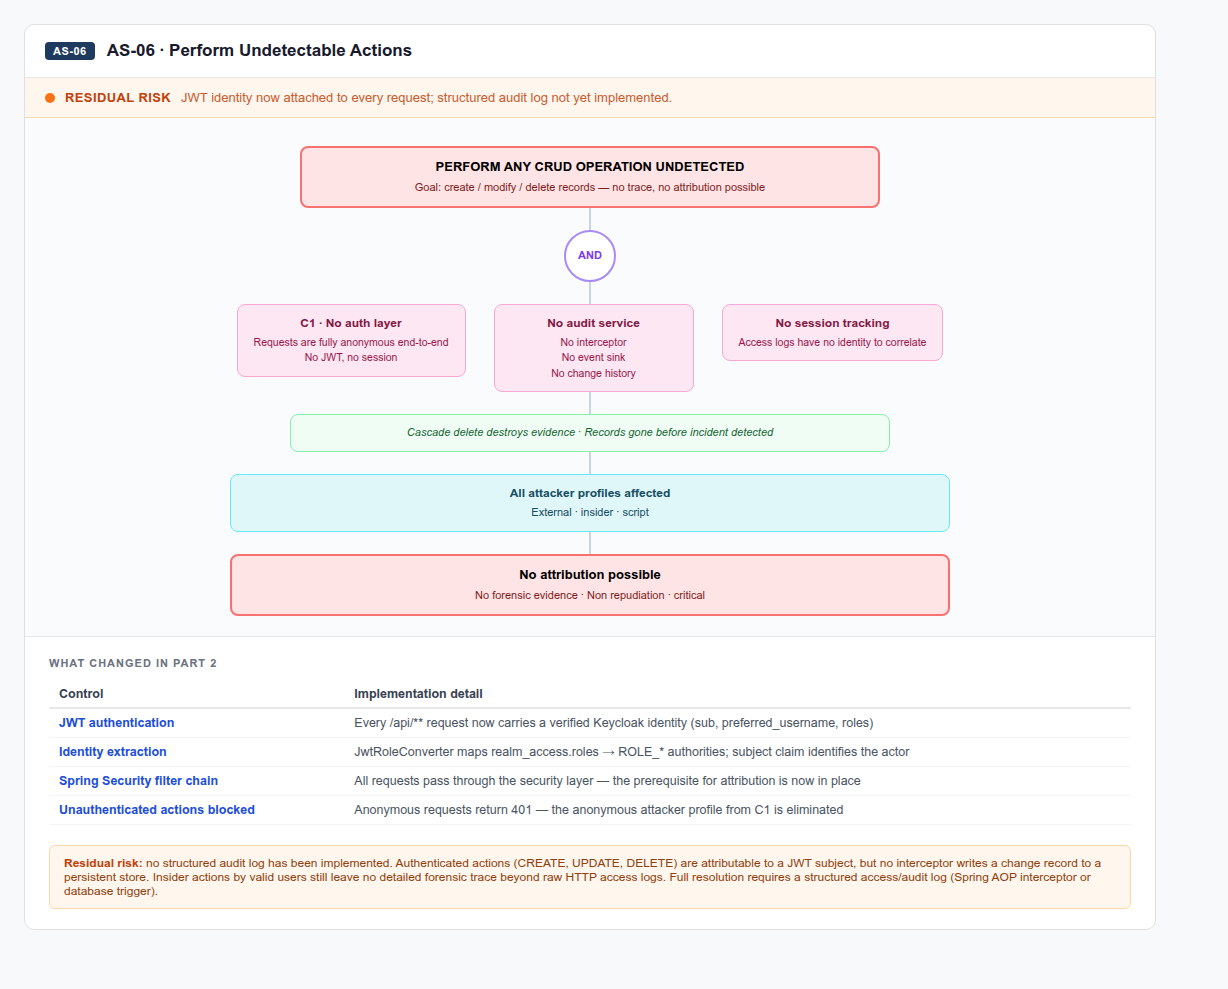
\includegraphics[width=\linewidth]{06_regression.png}
  \caption{AS-06 -- Destroy Patient Records via Cascade Deletion: \textbf{Prevented}}
\end{figure}

\begin{figure}[H]
  \centering
  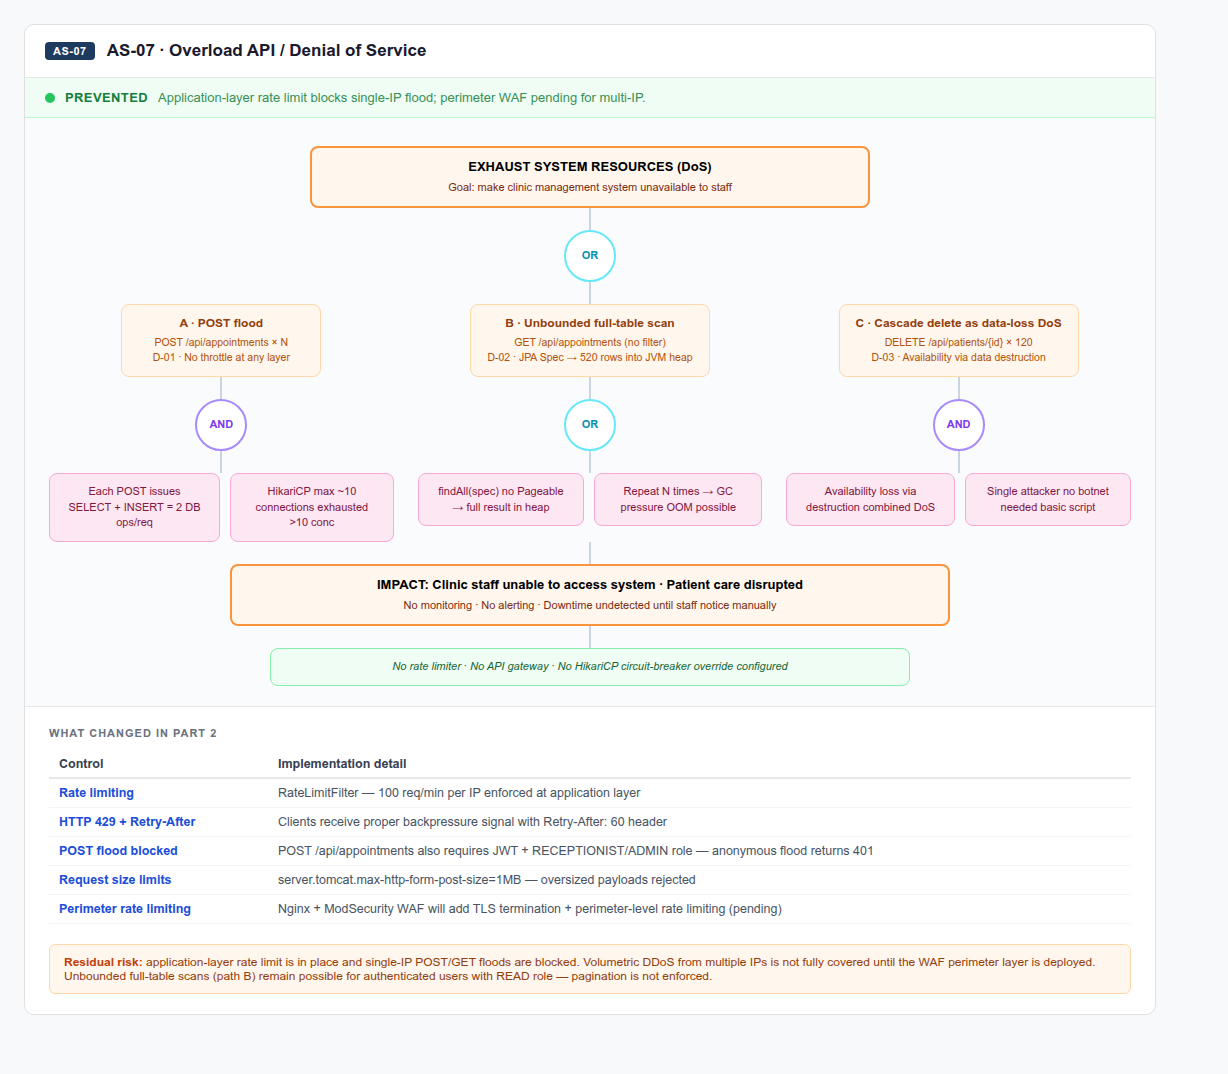
\includegraphics[width=\linewidth]{07_regression.png}
  \caption{AS-07 -- Undetectable Actions: \textbf{Detected}; AS-08 -- API Overload: \textbf{Prevented}}
\end{figure}

\subsection{Regression Summary}

\begin{table}[H]
\centering
\caption{Regression summary by status}
\begin{tabular}{lcc}
\toprule
\textbf{Status} & \textbf{Count} & \textbf{Abuse Stories} \\
\midrule
Prevented      & 7 & AS-01, AS-02, AS-03, AS-04, AS-05, AS-06, AS-08 \\
Detected       & 1 & AS-07 \\
Residual Risk  & 0 & -- \\
\bottomrule
\end{tabular}
\end{table}

Seven of the eight abuse stories are classified as \textbf{Prevented}; the remaining one
(AS-07) is classified as \textbf{Detected} -- actor identity and action are persisted in the
audit log, making post-incident investigation possible. No abuse story remains at Residual Risk.

% ─────────────────────────────────────────────────────────────────────────────
\section{Future Work}
% ─────────────────────────────────────────────────────────────────────────────

Two security improvements remain identified but not yet implemented.
Replacing sequential integer primary keys with \textbf{UUID primary keys} would eliminate the
ID enumeration vector exploited in AS-03, making brute-force IDOR significantly harder even
for authenticated callers. On the transport side, \textbf{mTLS for inter-service communication}
should extend TLS from the current WAF perimeter to internal container-to-container channels
(WAF $\to$ backend, backend $\to$ Keycloak) to fully satisfy ZTA tenet 2. Additionally,
\textbf{device posture} assessment -- integrating endpoint verification before granting access
-- is needed to address ZTA tenet 1.

% ─────────────────────────────────────────────────────────────────────────────
\section{Conclusion}
% ─────────────────────────────────────────────────────────────────────────────

This report documents the security improvements applied to ClinicWave during Part 2 of the
project, addressing the vulnerabilities and privacy threats identified in Part 1.

The baseline application had no authentication, no authorisation, and no perimeter controls,
leaving all patient and appointment data fully exposed. Part 2 introduced a layered defence
that closes all five high-severity attack paths identified in Part 1. Authentication is
enforced via Keycloak 26.2.5 with JWT RS256 tokens; a fine-grained RBAC model controls access
at the method level using \texttt{@PreAuthorize} annotations and a role-permission matrix
loaded from configuration. A perimeter WAF (Nginx + ModSecurity CRS in blocking mode, Paranoia
Level 1) filters malicious requests before they reach the application, provides TLS termination
on port 443, and enforces IP-based rate limiting in combination with the application-layer
\texttt{RateLimitFilter}. The OpenAPI specification documents all endpoints, and a two-run DAST
pipeline validates the security posture both with and without the WAF in place.

Of the eight abuse stories from Part 1, seven are now classified as \textbf{Prevented} and one
(AS-07) as \textbf{Detected}. Soft-delete prevents irreversible data loss from cascade deletion
(AS-06). The structured audit log makes every CRUD operation attributable and investigable
(AS-07). No abuse story remains at Residual Risk. The principal outstanding items are UUID
primary keys to harden IDOR resistance further, and mTLS for internal service-to-service
channels to fully close ZTA tenet 2.

\end{document}

